% concatenated from for-EAAMO.tex
%%
%% This is file `sample-manuscript.tex',
%% generated with the docstrip utility.
%%
%% The original source files were:
%%
%% samples.dtx  (with options: `all,proceedings,bibtex,manuscript')
%% 
%% IMPORTANT NOTICE:
%% 
%% For the copyright see the source file.
%% 
%% Any modified versions of this file must be renamed
%% with new filenames distinct from sample-manuscript.tex.
%% 
%% For distribution of the original source see the terms
%% for copying and modification in the file samples.dtx.
%% 
%% This generated file may be distributed as long as the
%% original source files, as listed above, are part of the
%% same distribution. (The sources need not necessarily be
%% in the same archive or directory.)
%%
%%
%% Commands for TeXCount
%TC:macro \cite [option:text,text]
%TC:macro \citep [option:text,text]
%TC:macro \citet [option:text,text]
%TC:envir table 0 1
%TC:envir table* 0 1
%TC:envir tabular [ignore] word
%TC:envir displaymath 0 word
%TC:envir math 0 word
%TC:envir comment 0 0
%%
%% The first command in your LaTeX source must be the \documentclass
%% command.
%%
%% For submission and review of your manuscript please change the
%% command to \documentclass[manuscript, screen, review]{acmart}.
%%
%% When submitting camera ready or to TAPS, please change the command
%% to \documentclass[sigconf]{acmart} or whichever template is required
%% for your publication.
%%
%%
\documentclass[manuscript,screen,authorversion]{acmart}

%\documentclass[manuscript,screen,review,anonymous]{acmart}
%\documentclass[acmsmall,screen,authorversion,nonacm]{acmart}

%%
%% \BibTeX command to typeset BibTeX logo in the docs
\AtBeginDocument{%
  \providecommand\BibTeX{{%
    Bib\TeX}}}

%% Rights management information.  This information is sent to you
%% when you complete the rights form.  These commands have SAMPLE
%% values in them; it is your responsibility as an author to replace
%% the commands and values with those provided to you when you
%% complete the rights form.
\setcopyright{acmlicensed}
\copyrightyear{2018}
\acmYear{2018}
\acmDOI{XXXXXXX.XXXXXXX}
%% These commands are for a PROCEEDINGS abstract or paper.


%\acmConference[EAAMO 2026]{Make sure to enter the correct
%  conference title from your rights confirmation email}{June 03--05,
 % 2018}{Woodstock, NY}
%%
%%  Uncomment \acmBooktitle if the title of the proceedings is different
%%  from ``Proceedings of ...''!
%%
%%\acmBooktitle{Woodstock '18: ACM Symposium on Neural Gaze Detection,
%%  June 03--05, 2018, Woodstock, NY}
\acmISBN{978-1-4503-XXXX-X/2018/06}


%%
%% Submission ID.
%% Use this when submitting an article to a sponsored event. You'll
%% receive a unique submission ID from the organizers
%% of the event, and this ID should be used as the parameter to this command.
%%\acmSubmissionID{123-A56-BU3}

%%
%% For managing citations, it is recommended to use bibliography
%% files in BibTeX format.
%%
%% You can then either use BibTeX with the ACM-Reference-Format style,
%% or BibLaTeX with the acmnumeric or acmauthoryear sytles, that include
%% support for advanced citation of software artefact from the
%% biblatex-software package, also separately available on CTAN.
%%
%% Look at the sample-*-biblatex.tex files for templates showcasing
%% the biblatex styles.
%%

%%
%% The majority of ACM publications use numbered citations and
%% references.  The command \citestyle{authoryear} switches to the
%% "author year" style.
%%
%% If you are preparing content for an event
%% sponsored by ACM SIGGRAPH, you must use the "author year" style of
%% citations and references.
%% Uncommenting
%% the next command will enable that style.
%%\citestyle{acmauthoryear}
% from informs template

% \usepackage{natbib}
%  \bibpunct[, ]{(}{)}{,}{a}{}{,}%
%  \def\bibfont{\small}%
%  \def\bibsep{\smallskipamount}%
%  \def\bibhang{24pt}%
%  \def\newblock{\ }%
%  \def\BIBand{and}%
 
 \usepackage{tikz,calc}
 \usetikzlibrary{decorations.markings}
 \usepackage{soul}
 \setul{}{0.75pt}
 \setuloverlap{1.5pt}


% \usepackage{subfigure}
% \usepackage{subcaption}
\usepackage{mwe}
\usepackage{lscape,booktabs,longtable}
\usepackage{amsmath}
%%\usepackage[pdftex,colorlinks=true,urlcolor=blue,citecolor=blue,pdfstartview=FitH]{hyperref}
\usepackage{comment}
\usepackage{enumerate}
\usepackage[ruled,vlined]{algorithm2e}
\usepackage[graphicx]{realboxes}
\usepackage{todonotes}
\usepackage{tabularx}

\newcommand{\rev}[1]{\textcolor{black}{#1}}


\usepackage{subcaption}
\newcommand{\modone}{\mod_{\hspace{-.04in}1\hspace{.04in}}}

\newcommand{\tr}{\textcolor{red}}
\newcommand{\tb}{\textcolor{blue}}
\newcommand{\tg}{\textcolor{mygreen}}

\newcommand{\E}[1]{{\mathrm{E}\left[#1\right]}}
\newcommand{\f}[1]{{\text{f}\left(#1\right)}}
\newcommand{\ind}[1]{{\,\mathbf{1}\hspace{-.025in}\left\{#1\right\}}}
\newcommand{\PP}[1]{\mathrm{P}\left( #1 \right)}
\newcommand{\Var}[1]{{\mathrm{Var}\left(#1\right)}}
\newcommand{\Cov}[1]{{\mathrm{Cov}[#1]}}
\newcommand{\T}{{\mathrm{T}}}

\usepackage{cleveref}

\usepackage{outlines}
\usepackage{tikz}
\usepackage{url}
\usepackage{xcolor}
\raggedbottom
\allowdisplaybreaks
\usetikzlibrary{arrows, positioning, shapes}
\tikzstyle{process} = [rectangle, minimum width=3cm, minimum height=1cm, text centered, draw=black, fill=white]
\tikzstyle{queue} = [circle, minimum size=1cm, text centered, draw=black, fill=white]
\tikzstyle{arrow} = [thick,->,>=stealth]


%%
%% end of the preamble, start of the body of the document source.
\begin{document}

%%
%% The "title" command has an optional parameter,
%% allowing the author to define a "short title" to be used in page headers.
\title{Due Process on Hold:
A Queueing Framework for Improving Access in SNAP}

%%
%% The "author" command and its associated commands are used to define
%% the authors and their affiliations.
%% Of note is the shared affiliation of the first two authors, and the
%% "authornote" and "authornotemark" commands
%% used to denote shared contribution to the research.
\author{Andrew Daw}
\authornote{Alphabetical order}
\authornotemark[0]
\email{dawandre@usc.edu}
\affiliation{%
  \institution{University of Southern California}
  \country{USA}
}
% \email{trovato@corporation.com}
% \orcid{1234-5678-9012}
\author{Chloe Pache}
\authornotemark[0]
\affiliation{%
  \institution{University of California, Santa Barbara}
    \country{USA}
}
% \affiliation{UCSB}
% \authornotemark[1]
% \email{webmaster@marysville-ohio.com}
% \affiliation{%
%   \institution{Institute for Clarity in Documentation}
%   \city{Dublin}
%   \state{Ohio}
%   \country{USA}
% }

\author{Angela Zhou}
\authornotemark[0]
\email{zhoua@usc.edu}
\affiliation{%
  \institution{University of Southern California}
    \country{USA}
}
% \affiliation{%
%   USC}
% \email{zhoua@usc.edu}

%%
%% By default, the full list of authors will be used in the page
%% headers. Often, this list is too long, and will overlap
%% other information printed in the page headers. This command allows
%% the author to define a more concise list
%% of authors' names for this purpose.
% \renewcommand{\shortauthors}{Daw et al.}

%%
%% The abstract is a short summary of the work to be presented in the
%% article.
\begin{abstract}
The U.S. social safety net delivers essential services at mass scale, but access burdens persist, as congested contact or call centers serve as a primary mode of application completion and assistance. In Holmes v. Knodell, Missouri’s SNAP call centers were so congested that nearly half of all application denials were procedural—caused by applicants’ inability to complete required interviews, rather than underlying ineligibility. The judge ruled these system failures led to a violation of procedural due process.
We propose a performance evaluation framework based on queueing models from operations research and management to assess and improve access in such systems. Operational access failures of call centers are distinct from prior automation failures in benefits provision. \textit{Emergent arbitrariness} arises from interactions between system dynamics and access demand, rather than from an explicit algorithmic rule, making diagnosis and repair inherently system-level. We develop a queueing model that incorporates phenomena that distinguish social services from standard service domains, redials and abandonment, through which backlogs generate \textit{endogenous congestion}. Standard queueing guidance from Erlang-A that does not address endogenous congestion fundamentally understaffs, which could lead to persistent shortfalls in practice. Using a fluid approximation, we derive steady-state performance metrics to analytically characterize the impacts of bundled staffing and service delivery changes. We fit model parameters to call-center data disclosed in court documents. Our queueing model can support ex-ante evaluation and design of access systems, inform policy levers for improving access, and provide evidence about whether applicants are afforded a meaningful opportunity to be served at scale.
\end{abstract}

%%
%% The code below is generated by the tool at http://dl.acm.org/ccs.cfm.
%% Please copy and paste the code instead of the example below.
%%
\begin{CCSXML}
<ccs2012>
   <concept>
       <concept_id>10010405.10010481</concept_id>
       <concept_desc>Applied computing~Operations research</concept_desc>
       <concept_significance>500</concept_significance>
       </concept>
   <concept>
       <concept_id>10002944.10011123.10011674</concept_id>
       <concept_desc>General and reference~Performance</concept_desc>
       <concept_significance>500</concept_significance>
       </concept>
   <concept>
       <concept_id>10002944.10011123.10011124</concept_id>
       <concept_desc>General and reference~Metrics</concept_desc>
       <concept_significance>500</concept_significance>
       </concept>
   <concept>
       <concept_id>10002950.10003648.10003688.10003689</concept_id>
       <concept_desc>Mathematics of computing~Queueing theory</concept_desc>
       <concept_significance>500</concept_significance>
       </concept>
 </ccs2012>
\end{CCSXML}

\ccsdesc[500]{Applied computing~Operations research}
\ccsdesc[500]{General and reference~Performance}
\ccsdesc[500]{General and reference~Metrics}
\ccsdesc[500]{Mathematics of computing~Queueing theory}

% \received{20 February 2007}
% \received[revised]{12 March 2009}
% \received[accepted]{5 June 2009}

%%
%% This command processes the author and affiliation and title
%% information and builds the first part of the formatted document.
\maketitle



\section{Introduction}

% \section{Background}

% \paragraph{Background on SNAP} SNAP. block grants. decentralized administration by states/counties. 


%In recent years, there has been a renewed focus on service delivery in the public sector. Many social service organizations, such as government entities and nonprofits, provide essential or supportive services to large swathes of the population. The private sector has developed advanced, seamless, technology-based platforms tailored for frictionless customer experiences. On the other hand, increasing scholarship in public administrative recognizes the challenges of ``administrative burden," meaning the requisite learning, psychological load, and compliance costs that citizens experience in interactions with government. These burdens can block citizens from accessing the services they need. 

Social safety net programs deliver essential services and benefits at a massive scale under major resource constraints. Operational challenges in service delivery can undermine efforts to achieve policy goals and program effectiveness. Recently, a district court case, \textit{Holmes v. Knodell}, ruled that Missouri Department of Social Services’ (DSS) Supplemental Nutrition Assistance Program (SNAP) call center was so congested that enrollees were unable to call through to complete required interviews and applications, constituting a procedural due process violation.
\textit{Procedural denials} occur when an application is denied purely on procedural or administrative grounds, such as missing an interview, rather than the eligibility facts of the case. In Missouri, such procedural denials were as high as 50\% of all denials. %The high rate of procedural denials --- 50\% --- indicates that operational failures such as long wait times prevent potentially otherwise eligible individuals from accessing crucial benefits.
To the best of our knowledge, this is the first time that an \textit{operational system (the call center) was found to violate procedural due process}. While the case ruling has concluded, the story is not complete. Missouri DSS has been ordered to improve call center operations under severe staffing constraints, reflecting a broader challenge across public-sector service delivery: how to provide meaningful access at scale with limited resources. How should Missouri DSS improve their call center design to provide \textit{de facto} access to complete \textit{de jure} application requirements? 

% Call centers are the primary access mode for SNAP, like other social service programs. 
%We focus on the specific setting of call centers for providing interviews for SNAP (Supplemental Nutrition Assistance Program, formerly known as food stamps) recertifications (renewals). 
%Recently, a district court case, \textit{Holmes v. Knodell} ruled against Missouri Department of Social Services. 

% Enrollment for, and recertification (renewal) of, SNAP requires an interview with a caseworker to go over fine-grained details particular to program eligibility. Federal guidelines require interview completion within $30$ days; however, call centers, like other operational infrastructure in the social safety net, are under-resourced and are understaffed. 

%NHElP legal aid argued that the high rate of procedural denials --- 50\% of all denials --- represented a procedural due process violation on Missouri DPSS' part to provide an operationally viable implementation of their enrollment pathways, in order to implement federal policy. 

 %Unlike prior automation failures in benefits provision, long call center wait times that block individuals from talking to a representative cannot be traced back to a single system design choice or implementation failure. Instead, long wait times emerge from a sociotechnical system with interacting technical queueing system design, enrollee demand and enrollee behavior. 

%The \textit{cooperative federalism} of benefits administration --- funded and regulated by the federal government, but administered by states --- results in wide operational variation and unclear technical guidance. 

The operational failures of long wait times in automated systems are systemic both in \textit{origin} and \textit{future improvement}, differing from prior automation failures in benefits provision. We do not find available technical guidance that addresses the specific challenges of social service delivery. %that has long studied probabilistic modeling of service systems, meaning systems in which customers may wait for access to limited goods, resources, or providers --- including call centers. %Originally dating from the analysis of Copenhagen's telephone network over a century ago, this field has produced models and insights which have been widely employed for the design and control of service systems in practice. Accordingly, these stochastic processes have been the subject of myriad studies in the literature, ranging from deeply theoretical analyses of the models rigorous applications to real-world settings. 
% Accordingly, modern call centers have grown increasingly complex in their operations, and this sophistication has thus demanded a similarly rich understanding of a given system's performance, with many details varying significantly from one implementation to the next. 
Queueing theory, which is a key subdiscipline of operations research, is the natural tool for performance analysis. Call centers have been a particularly fruitful domain, as they feature the core ingredients of the field: large volumes of customers, random fluctuations in the times between arrivals and the durations of service, and strong potential for long wait times despite the risks of impatient customers. 
Indeed, federal guidelines for performance management of SNAP call centers refer to queueing theory and mention the famous Erlang-A formula, while also conceding that the \textit{specific} nature of social services means that standard off-the-shelf models may not directly apply; hence, the assumptions for the Erlang-A formula do not actually hold in practice \citep{fns}. 

Here, we develop a queueing model to fill the gap between standard call center models and special challenges in social services. %We develop a \textit{queueing model and framework} for the performance evaluation and improvement of call centers for benefits provision.
Call centers for SNAP, and benefits more broadly, specifically suffer from \textit{abandonment} where busy callers, some of whom may be paying by the minute \citep{howe_new_2025}, cannot stay on hold forever and may drop their call. But, the key difference from standard models is that callers applying to satisfy SNAP interview requirements who abandon are likely to call back, or \textit{re-dial}, since SNAP and other social safety net programs serve urgent needs without private outside options. Moreover, interviews often surface additional follow-up steps resulting in future calls. These behaviors, distinctive to social services, \textit{compound operational deficiencies}, introducing stark feedback loops where prior backlogs result in abandonment that only worsens future congestion due to re-dials. Our model captures these distinctions and is therefore relevant beyond SNAP alone, for example for backlogs for unemployment insurance or Social Security Administration (SSA) call centers, which have suffered major backlogs and similar high-abandonment issues at times including prior economic crises \citep{pahlka2023recoding,Coffey_2017,ho2025evaluation} and current understaffing \citep{Rain_Natanson_25AD}.

% Our model can be helpful beyond the administration of SNAP alone. Other programs also rely on call and contact centers, just as major enterprises do, to serve as an interface with a massive client base. In practice, backlogs and queues in accessing government services comprise major crises in administration and service delivery. Unemployment insurance suffered major backlogs in disbursing benefits and call center waits during the Great Recession in 2008 and during the COVID-19 pandemic \citep{pahlka2023recoding,Coffey_2017,ho2025evaluation}. In 2025, backlogs grew for the Social Security Administration (SSA) amid chaotic changes in field operations at SSA offices and chronic understaffing \citep{Rain_Natanson_25AD}; agencies reported an average speed to answer that excluded the wait time for a callback (1-2 hours on average) while around 25\% of calls were abandoned. 


\rev{We focus on a fluid approximation of the queueing model, which is a deterministic approximation to the queueing system under large arrival volumes and with many servers, both of which are evident in the  SNAP call center data from \emph{Holmes v. Knodell} \citep{holmesKnodellPlaintiffsMSJ2024}. Agencies could use our framework to understand trade-offs between different call center system design choices and resource expenditures. Our analysis in the fluid model enables us to vary system parameters and answer questions such as  ``if I can only hire 10 more staff, by how much would I have to reduce handling time in order to reduce wait time below 20 min?'' To preview how this can be useful, first we note that DSS estimated that they needed at least 150 more staff\footnote{\rev{DSS had 200-300 staff split among different tasks including handling calls and scheduled interviews, but the agency had earlier estimated that they needed >400 staff dedicated to answering calls alone to answer 80\% of calls within 2 minutes \citep{holmesKnodellPlaintiffsMSJ2024}.}}, most likely using the Erlang A formula, which is the only the only operations guidance we see in federal documents \citep{fns}. But DSS already faced difficulties with retention, let alone hiring and onboarding new staff which takes a long time and may not grant immediate relief. Our quantitative model shows the same performance improvement can be achieved by \textit{bundling operational changes} with fewer additional staff. In SNAP, the Erlang-A's model assumption of permanent abandonments fundamentally fails: applying callers don't have outside options, so abandoned calls turn into re-dials, and therefore congestion itself generates future arrivals. Our finer-grained model includes the \textit{endogenous congestion} generated by re-dials and includes key dynamics that arise from program design and implementation. Accordingly, using our model, policymakers can directly assess \textit{how changes in program implementation and operations} (such as changes in timeframe for obtaining follow-up documentation) affect system performance. }


The focus of our work is in developing a performance evaluation and improvement framework, expanding upon classical queueing models from operations research, that can support efforts to  improve access in social services. Our model, though reliant on some probabilistic assumptions, allows us to estimate \rev{six key performance metrics: the mean number of waiting callers, the mean waiting time, the average speed to answer (i.e., the waiting time for callers who don't abandon), the procedural denial rate, the endogenous congestion from re-dials, and the endogenous congestion from re-certification. The first three waiting-based metrics are hallmark measures of performance in essentially any call-center, and the latter three are specifically relevant in this SNAP call center setting, where the dynamics of the benefits certification process creates patterns of returning callers that can magnify the load on the system and are not typical in other call center settings.}
%like wait times, abandonment (informative of procedural denials), throughput, and others, under changes in system parameters. 
The queueing model captures the \textit{feedback loops} that arise when relying on call centers for required interviews and re-certifications that themselves generate follow-up contacts. %Although a theoretically simple fix is to just hire more staff until backlogs are cleared, in practice, inevitable resource, training and hiring constraints require exploring other system design changes. 
We introduce our queueing model, its fluid approximation, and discuss how to calibrate the model to data, which we do using court documents from \textit{Holmes v. Knodell}. We introduce a simple dashboard to explore the impact of design changes on performance metrics. Our model admits analytical expressions for \rev{the six focal performance metrics}, which we analyze to obtain insights on how different design changes impact performance. \rev{Furthermore, the dashboard demonstrates how the model also lets us evaluate many other quantities beyond the six highlighted in the paper.} Finally, we use our calibrated model to illustrate how an agency might combine staffing and system/policy design levers, like reducing average handling time or lengthening re-certification cycles, in order to achieve greater improvement with less staffing. 
% such as re-dialing to satisfy mandated interviews, shorter 6-month recertification cycles with interview, or abandonment further increase system congestion, even beyond other typical call centers.

%Just to name a few: while in general, waiting or queueing burdens can be a way to screen customers for the highest utility to target those who might most benefit, the theory of administrative burden suggests that those who most benefit are those who might lack the means or resources to navigate these burdens. 
% And, any operational inefficiencies in accessing social services or case management only compound: since these programs serve urgent needs, and there are no private outside options, the only recourse customers have is to call back. 

% The focus of our work is in providing 
% Importantly, given this legal context, and given the court's decision calling the overwhelmed call center a due process failure, the question of appropriate redress concerns \textit{improving} performance to remove such arbitrary barriers to access. 
% The court's decision introduces some natural compartmentalization between legal and technical concerns: Missouri DSS's task now is to improve call center operations 
%This introduces some natural compartmentalization between legal and technical concerns. We introduce our queueing framework to model how the specific program design affects the operational dynamics.  Queueing models provide a crucial tool for the operations of access. Importantly, congestion, abandonment of queues, and other systematic failures are predictable and measurable. System design exercises that manipulate queueing models can provide guidance as to administrative alternatives that can improve access. Performance management and evaluation of system performance is a basic pre-condition for improving due process when algorithmic systems are part of the administration of state resources. 


% This is exactly where our formal queueing model comes in. Looking at FNS guidelines, we at least find little fine-grained technical guidance as to how to design call centers in light of calling behaviors that arise in the provision of social services. FNS guidelines refer to a classical Erlang-A staffing formula and more broadly to the field of simulation. While we are unaware of more specific guidance within the third-party Genesys call center system either, it remains unlikely that Genesys’ underlying models specifically account for calling behavior in the provision of social services either. Specifically: we anticipate significant abandonment (given the administrative burdens and potential volatile working schedules or household obligations) as well as re-dials, individuals who call the call center again since they must have an interview rescheduled (or they are following-up with additional documents). Our formal models can provide approximate guidance as to which changes in system design could lead to improved performance (lower wait times). Our models can also highlight how behaviors that are more specific to the urgency in accessing social services or administrative burdens, such as re-dialing to satisfy mandated interviews, shorter 6-month recertification cycles with interview, or abandonment further increase system congestion, even beyond other typical call centers. [[cite sludge]]
\section{Background}
\paragraph{Background on SNAP}
The Supplemental Nutrition Assistance Program (SNAP), formerly the Food Stamp Program, is the largest means-tested social assistance program in the United States and provides monthly food-purchasing benefits to low-income households. SNAP is federally authorized and funded but administered by state and local agencies, which are responsible for determining eligibility and operating application and recertification processes within federal rules. In fiscal year 2024, ``SNAP served an average of approximately 41.7 million individuals per month—about 12.3\% of the U.S. population" \citep{ers_snap_key_stats}.\footnote{Participation by state varies widely, from as high as 21.2\% in New Mexico to 4.8\% in Utah \citep{ers_snap_state_variation}.} Studies of SNAP and other benefits programs find improvements not only in food security, but also health and labor outcomes, as well as stabilization against macroeconomic downturns \citep{hoynes2015us}. Nonetheless, many who are eligible for SNAP do not receive benefits. Program eligibility is complex, including income determination and verification, deductions, asset limits, household definition, and work requirements --- as is the application \citep{crs_snap_r42505}. Such complexity introduces ``administrative burden,"  the requisite learning, psychological load, and compliance costs that citizens experience in interactions with government \citep{herd2025administrative}. 
Many who are denied benefits because of operational frictions (missed interviews, application errors) are actually eligible \citep{homonoff2021program}. %``In 2019, one third of all
% applications in Los Angeles County were denied due to a missed interview," while five times as many were denied for ineligibility. 


\textit{The role of the interview, applications and recertification process: } Call and contact centers remain one of the primary ways that potential enrollees interact with SNAP program administration \citep{fns}.\footnote{Services provided by call centers can provide everything from general information to official case services like updating and processing changes, conducting interviews, providing updates on processing, appointment scheduling and more. Staffing SNAP call centers is difficult because of SNAP policy complexity and the need to access live case information; call center staff touching the eligibility process must be merit system personnel \citep{fns}. As a result, there is large turn-over and chronic under-staffing, and it can take a long time to onboard new staff  \citep{Coffey_2017} --- Missouri DSS faced these challenges as well.} 
Key administrative \textit{checkpoints} \citep{kim2025administrative} in the SNAP process include initial application, which requires an interview, and re-certification every 6 to 12 months, which also requires an interview. The re-certification form measures changes of circumstances (including costs/income, household composition, etc.) %\footnote{for example, in lodging and housing costs, household composition, income, schooling status of income, food preparation household determination, income proof for individuals in food-preparing household, proof of benefits recipience, proof of changes in care/health expenses} 
which may change eligibility; any changes require submitted verification. During interviews, the caseworker may ask for additional documents to prove certain eligibility requirements or provide additional detail. Initial interviews also often serve as opportunities to inform applicants about complex SNAP-specific definitions. %Some jurisdictions grant at least a period of at least 10 days to collect this additional information \citep{BenefitsCal}.


Missouri DSS has a waiver from Food and Nutrition Services (FNS), the federal agency administering SNAP, to implement interview procedures deviating from federal guidelines - namely, DSS does not need to schedule interviews, but must provide applicants with a notice (interview letter) instructing them to contact the Call Center within 5 days of submitting their application. If they do not, they receive a notice of missed interview informing that they need to complete the interview within 30 days of submitting their application. 

More broadly, there are no uniform performance standards for operational performance for interviews.\footnote{\citet{howe_new_2025} comment on the legal context of \textit{Holmes v. Knodell} and the challenge of rendering on-the-ground wait times legally cognizable. Existing enforceable laws did not anticipate the omnichannel service and access needs of today's day and age.} Although interviews are \textit{required} by federal regulation to be completed within 30 days, federal regulation does not stipulate performance standards on service quality of \textit{how} interview opportunities should be granted to enrollees. It remains unclear what \textit{exact} metrics might lead to judicial findings of procedural due process violations.\footnote{For example, the judge noted that in Missouri near 50\% of denials were procedural. But other jurisdictions also have high rates of procedural denials that reflect persistent access barriers; for example, Los Angeles in 2018-2019 had a baseline rate of $\sim30$\% procedural denials \citet{giannella2024administrative}.} 

\textit{The grounds for the judicial decision:} 
% The judge concludes that
The case facts establish that the call center and administrative process (including low-staffed resource centers) to handle SNAP applications are overwhelmed. Plaintiffs contend that wait times are unacceptable, with some plaintiffs calling ten to twenty times and unable to call through, and legal services advocates waiting in the queue for hours before getting disconnected \citep{holmesKnodellPlaintiffsMSJ2024}. DSS is understaffed.\footnote{DSS has 200-300 staffers split in between informational (non-interview) calls and interview calls, while it estimates it needs 400 interview-only staffers to meet private call center “industry standards” of answering 80\% of calls within 2 minutes} Thirty-two percent of all calls that made it into the interview-only queue were abandoned by the caller. Fifty percent of all applicants were denied for failure to complete the interview in one month during 2023, due only to a failure of the system to offer a reasonable opportunity to interview. % Per the order granting plaintiffs' motion \citep{holmesKnodell2024}, ``Federal law requires Defendant to provide timely, accurate, and fair service to applicants for, and participants in, the SNAP program...  The changes, modifications, and adjustments made by DSS after increasing its reliance on its telephone system to process SNAP applications have proven unsuccessful in fulfilling Defendant’s responsibility to provide timely, accurate, and fair service for applicants and participants in the program.'' 
The judge concludes that DSS was unsuccessful in providing ``timely, accurate and fair service,'' that the ``reliance on an inadequate automated system and understaffed offices to provide interviews also violates Defendant’s obligation under SNAP and Defendant’s on-demand waiver,'' and therefore    denial based on the automated system is a wrongful denial of benefits based on the arbitrariness of whether enrollees can call through \citep{holmesKnodell2024}.\footnote{``Here, applicants are being denied benefits not based on the merits of their application but on the failure to obtain an interview. Further, the failure to interview is a direct result of Defendant's inability to provide an efficient and successful system that allows applicants to schedule and complete an interview within the required time frame.'' \citep{holmesKnodell2024}} 
%Holmes, 2024 WL 2097081, at *1 (“These denials were not based on the merits of the applications but the failure of the system to offer a reasonable opportunity to interview.”); id. at *12 (“Too many applicants are rejected based on the failure of the system, rather than substantive evaluation of the applications.”); id. at *16 (“[A]pplicants are being denied benefits not based on the merits of their application but on the failure to obtain an interview. Further, the failure to interview is a direct result of Defendant’s inability to provide an efficient and successful system that allows applicants to schedule and complete an interview within the required time frame.”).




\textit{Background on procedural due process:} Much prior work in the algorithmic fairness community has focused on connecting algorithmic harms or performance legal theories of discrimination. \textit{Holmes v. Knodell} is a \textit{procedural due process}\footnote{\textit{Procedural due process} requires that the state follow certain procedures when depriving someone of their property, such as giving notice, an opportunity to be heard (for example, in court), and a neutral decision-maker  \citep{ames2020due}. %Procedural due process applies also to administration of the social safety net and welfare. 
Courts have ruled, since the Goldberg v. Kelly, 1970, Supreme Court case, that social safety net and welfare programs represent significant property interests and hence are subject to procedural due process protections. 
% \textit{Procedural due process} requires that the state follow certain procedures when depriving someone of their property (or life or liberty): it must provide notice, give an opportunity to be heard (for example, in court), and provide a neutral decision-maker. Procedural due process applies also to administration of the social safety net and welfare, since an influential ruling in Goldberg v. Kelly []. 
Traditionally, such protections, drawing upon due process in courtroom procedures, might take the form of adversarial hearings, appeals, tribunals, or legal representation. } case, like other cases of algorithmic harms in benefits provision.  
% The term ``due process" conjures images of courtroom back-and-forth, governing adversarial courtroom trial procedures to ensure all actors' rights are preserved. But \textit{procedural due process} 
% But, when it comes to administering the social safety net, including government-administered programs with broad participation, traditional courtroom proceedings like hearings, tribunals, and legal representation %[https://www.law.cornell.edu/wex/procedural_due_process]
% are impossible to administer at scale. [SNAP scale] 
Scholars in administrative law have argued that such post-hoc appeals and hearings may not provide strong enough procedural protections for the massive scale of social safety net programs. \citet{mashaw1973management} studies the Social Security Disability Insurance (SSDI) program and adjudication process and argues for the ``management side of due process.'' %highlighting a key tension between individuated case management and analysis, and the ``bureaucratic rationality" of rules and standardization that might curtail discretion, and articulating a ``management side of due process". 
Mashaw argues that burdensome appeals surface a small fraction of the agency's actual errors. Instead, fairness, accuracy, and timeliness are properties of \textit{system performance}, not just rare appeals. Pro-active \textit{continuous monitoring and performance management} can provide more systematic guarantees than individualized procedure that is overly reliant on ex-post correction. {Fairness and accurate determinations are therefore emergent property of a system's performance as a whole, not necessarily individual procedural protections}. %For example, quality assurance at SSA comprises of random sampling for a second adjudication, as well as error analysis and monitoring. %Examples include SSA's quality assurance processes, where some cases are randomly sampled for a second adjudication, and error analysis and monitoring. 
\citep{ho2017managing,ames2020due} connect these arguments about performance management and quality assurance programs in agencies %conducting mass adjudication (immigration court, VA and veteran's benefits, SSA) in greater detail. These arguments resonate 
with modern calls for AI auditing, algorithmic accountability, and performance management, including \citep{ho2025evaluation} an example audit of benefits-assistance chatbots for UI assistance.%  \citet{ho2025evaluation} analyzes the role of administrative law in governing the emerging use of AI in benefits adjudication, with an example audit of recent state-deployed chatbots for assistance in unemployment insurance benefits. 

We share a similar high-level emphasis on \textit{the role of performance evaluation in operationalizing due process in benefits provision}. However, we focus specifically on call center performance, which introduces distinct technical challenges. %Mashaw highlights the role of quality assurance processes in SSDI, where some cases are randomly selected and re-analyzed to 


% alternative views

% Many raise fundamental concerns, including due process re: the legitimacy of using automated black-box systems at all to make eligibility determinations \citep{de2024inescapable}. But, the challenge of scale still remains -- full, careful and complete consideration of individualized circumstances is unlikely in perpetually funding-restricted environments. 


% [[ What's new about this setting]] 

% \paragraph{Administrative burdens}


%Mashaw argues that in mass welfare systems, due process must be understood as a problem of institutional management and quality assurance, not merely hearings and appeals, because only systemic monitoring can reliably protect claimants from error.

\paragraph{Emergent systemic arbitrariness from automated systems.}
Automated systems have introduced great harms in crucial social safety net programs and benefits provision \citep{eubanks2018automating,btah,richardson2019litigating}, due to flawed data, problematic system design choices, or inherent system limitations \citep{gules2025algorithmic}. %overviews court dockets contesting algorithm-based determinations in disability, unemployment, and nutrition assistance programs and taxonomizes issues as flawed data, problematic system design choices, or inherent system limitations.
%A number of prior cases have studied due process and automated decision-making, or more specifically, the role of automated systems in the provision of benefits. 
% A number of prior cases of automation occur due to specific technical ``errors" in \textit{de facto} technical implementation that directly violate \textit{de jure} due process requirements. However, 
\textit{Holmes v. Knodell} introduces new challenges because the problematic service deficiencies, like long wait times and inability to reach a live representative, are systemic consequences of the automated system, rather than a singular ``incorrect" algorithmic rule or implementation quirk that clearly violates procedural due process protections. %It's not clear that there's a specific \textit{system design choice} that violates procedural due process protections. 
We call this \textit{emergent arbitrariness}, which differs from other algorithmic failures in benefits teach where algorithmic rules directly violate \textit{de jure} procedural due process (e.g., defective notice or fully automated determinations).
% The judge's comparison to \textit{Barry v. Lyon} %\footnote{ In Barry v Lyon, the court ruled that Michigan Department of Health and Human Services must stop automatic denial of SNAP applications based on an automated match with a list of outstanding felony warrants (rather than those actively fleeing/actively being sought by law enforcement), which included erroneous matches such as aliases given by others or cases of identity theft. } 
% when interpreting the SNAP Act’s prohibition on wrongful denials highlights how  \textit{emergent arbitrariness} differs from prior system design failures that resulted in arbitrary agent actions.
In a referenced prior case as reference for arbitrary agency action, Barry v. Lyon, an added automated match imposed an extra eligibility requirement beyond those federally mandated, violating the SNAP Act. Yet, the fix is simple --- remove the automated match. In contrast, for SNAP call centers, the \textit{origins of} and \textit{future improvements} for the \textit{emergent arbitrariness} are more complex than a single system design flaw. The judge can mandate that Missouri DSS must modify its administration process to ensure the opportunity to interview, but it remains unclear \textit{how}.

%We argue that in \textit{Holmes v. Knodell}, the connections between the automated/technical system and the resulting \textit{arbitrary agency actions} that violate procedural due process protections  is distinct. %The  weighing in on the systemic failure of the operational call center system more broadly. Said differently, 
%In the case of the queueing call center, there is not necessarily just one aspect of system design that is the ``smoking gun" leading to overall \textit{systemic failure of inaccessibly long call wait times}. 


% \footnote{A first question is - what exactly is the automated system at fault here? On the one hand, one might object to the \textit{automatic denial} of applications in 30 days, even from those who try to call in to interview, and keep applications alive for those who try to call in (stay the denial). %But to change the 30-day automatic denial appears to be a non-trivial change to federal categorical eligibility guidelines, even if we agree such a change is more compatible to fundamental fairness.
% %removing the 30-day automatic denial is a non-trivial change to a current federal requirement, and therefore unrealistic for injunctive relief. 
% But without also improving system throughput, staying application denial without improving wait times only delays the ultimate approval of crucial benefits to enrollees.}. The call center system has some automated routing that implements sytem design. But we argue that the \textit{systemic long wait time outcomes} of the call center emerge from complex interactions between demand (inflow of individuals applying for or recertifying SNAP), system design (automated procedures that dictate how incoming calls are routed), and caller behavior (re-dialing when unable to connect for an interview or abandoning calls). 
%We term this systemic dependence as \textit{emergent arbitrariness} to distinguish from system failures where algorithmic implementations map directly to arbitrary agency actions that violate \textit{de jure} procedural due process protections, such as providing adequate notice or making determinations without human oversight.
% We argue that a queueing and systems analysis framework instantiates the broader \textit{performance management and evaluation for due process} \citep{mashaw1973management,ho2025evaluation} paradigm for service operations provisioned by call centers. Unlike prior cases on automation failures in benefits provision, there's not one single agency action, algorithmic implementation, or design choice that led to the call center congestion and consequent wait times\footnote{To be sure, some specific details of DSS' system design sound excessive, such as blocking or disconnecting all calls based on a crude approximation of the wait-time and extra padding of two hours, or the appointment scheduler that can’t be accessed until making it into the queue (i.e. not getting deflected/redirected). But, in general it’s unclear that changing any single one of these system configurations would improve system performance to clear backlogs, either.}. %Another suggestion is to increase staff, but DSS has already mentioned issues recruiting, not to mention ultimately limited budgets. The key question remains: So what exactly about the system should the agency change to grant a reasonable opportunity to call in for an interview? 
% While the conclusion is clear that procedural denials due to inability to call through for an interview constitute arbitrary denials, and hence “arbitrary agency action”, it’s not that the agency was explicitly making arbitrary actions for each individual case. It’s therefore difficult to pinpoint a single agency action or design choice that led to the arbitrary agency denials rather than the consequential system outcomes. 


% \paragraph{Administrative burdens}



  

\section{Related Work}


% \paragraph{Backlogs and queues in government services}

% Classical economic models conceptualize ordeals in accessing resource transfers as an essential component of \textit{targeting} transfers to just those individuals with the highest need, without private outside options \citep{nichols1982targeting}. 


\textit{Informal and formal performance evaluation of government benefits systems:}  
In formal quality control processes for SNAP, FNS collects random samples of household case files and analyzes eligibility determinations and overpayments/underpayment errors \citep{snapqc}. However, these formal performance evaluations focus on payment errors, rather than other system performance measures including administrative burdens, access, or other measures of otherwise-eligible households that nonetheless do not complete applications or receive benefits. Regarding call center performance specifically, there is wide heterogeneity in evaluation structure and specific metrics used across different government agencies and programs. (See \citet{Coffey_2017} for an overview for unemployment insurance\footnote{The Department of Labor contracted a consulting firm to survey different state leaders about their operational practices in call centers for unemployment insurance. They found wide variation in exact operational practices, but common use of strategies like cross-training and pooling queues across multiple call centers, while finding that many states could use more forecasting and queue management tools \citep{Coffey_2017}.}). However, the IRS has long provided assistance to tens of millions of Americans by phone, and has long designed its own call center quality and customer experience evaluations \citep{rosage2004evolution}.  %While most states (around three-quarters) reported efficiency metrics such as wait time, average speed to answer, and abandoment, far fewer (less than half) reported service levels that are standard in the private sector, like requiring $80\%$ of calls to be answered within $20$ minutes. 
In the absence of formal performance assessments and real-time reporting, outsiders may also run informal audits to report performance metrics\footnote{Earlier iterations of the IRS' call center evaluation included "mystery-shopper" like programs, with the downside that queries are artificial rather than actual customer concerns \citep{rosage2004evolution}.} \citep{dube2021note}.
% in a "mystery shopper" approach, recruited research assistants to call various state unemployment call centers during the COVID-19 pandemic to assess how long it took to get a live representative on the line, to quantify the backlog and access issues. 
Sen. Elizabeth's Warren's office made hourly calls to SSA, finding wait times of 100 minutes and that only 50\% of calls connected to a live representative \citep{warren}. Specifically in the context of \textit{administrative burdens and SNAP}, recent works study changes in interview operations that introduce or improve administrative burdens, demonstrating beneficial impacts of interview flexibility on approvals and long-term participation \citep{giannella2024administrative,kim2025administrative} or barriers from less time to reschedule \citep{homonoff2021program}.\footnote{\citet{homonoff2021program} find that later recertification interviews, with less time for rescheduling, decrease recertification success, including for truly eligible clients. % Interview inflexibility imposes greater administrative burden rather than efficient screening for the needier. 
\citet{giannella2024administrative} study a field experiment of applicant-initiated \textit{flexible} on-demand interviews in Los Angeles, increasing approvals by $6\%$ and long-term participation by $2\%.$ \citet{kim2025administrative} run a field experiment comparing text-message reminders of flexible interviews vs. mailed reminders in Boulder County, Colorado, finding earlier and 10\% more likely interview completion.  }

\textit{Other operational analysis of public-sector queueing systems:} 
Queueing analysis is a mature discipline, and prior studies have also focused on public sector systems, albeit not the SNAP access system here. Some prior studies focus on operations in the judicial case management system. \citet{freund2024dedicated} study the queueing system in immigration courts and analyze fairness/efficiency properties of the queueing discipline, as well as strategic considerations specific to when waiting provides utility \citep{freund2025regulating}. \citet{bakshi2025service} study delays in judicial case management. Judicial case management differs from our eligibility/administrative burden setting: in court docket management, cases stay ``live'' for extended periods of time, while for social services, the interview requirement must be completed within 30 days. \citet{anunrojwong2023information} study information design in a general model to target high-need individuals without outside options to manage a congested queue for social services. 

Although classical literature on ordeal mechanisms \citep{nichols1982targeting} posits that ordeals serve a targeting function to dissuade those who are ineligible, the reality of the situation is that administrative burden \citep{herd2025administrative} often prevents actually-eligible individuals from taking up beneficial services \citet{homonoff2021program}. \citep{garg2025heterogeneous} outlines empirically documented gaps in participation and access in other mechanisms.Our recommendations focus on bundled staffing and service delivery interventions that can mitigate current severe blockages in access, rather than achieving finer-grained targeting, which is an interesting question for future work. 

\rev{\textit{Welfare implications of queueing-mediated service provision:} Many service and health interventions in general experience capacity constraints, though this may not be explicitly modeled in explicit system or causal analyses of performance \citep{miles2019causal,boutilier2024operational}, introducing potential social welfare risks in scale-up of otherwise beneficial social interventions. \citet{liu2024redesigning} study service-level agreements under exogenous demand arrivals in municipal operations in a queuing model.
}

 \textit{Other technical work and benefits provision:} \citet{pahlka2023recoding} provides an overview of civic tech and digital services in the federal government, including key benefits tech infrastructure. \citet{escher2020exposing} audits benefits \textit{eligibility calculators} for potential errors. \citet{jo2025ai} explores AI and trust in LLM chatbots supporting SNAP applicants. \citet{koenecke2023popular} audits ad allocation budgets for SNAP outreach and in a survey, finds broad support for equity considerations. Recent evaluations of LLM and chatbots in social services include an audit of UI chatbot support \citep{ho2025evaluation} and \citet{gosciak2026llms} evaluates LLM-chatbot assistance for caseworkers in a randomized-controlled trial, finding that such chatbots can support caseworkers in answering factual questions when they are accurate, but optimal AI-human assistance strategies remain crucial. Recent interest in AI surfaces new opportunities for service redesign that could result in shorter service times or self-service channels, and can be represented in our framework as changes in model parameters. 


 
\section{Queueing Model}

%\paragraph{What's new in social services that differs from standard queueing: re-dials and abandonment}

%\paragraph{Abandonment}

%\paragraph{re-dials, short and long}

%Call centers are perhaps the foremost application of queueing models in practice. In addition to exhibiting key model assumptions like randomness in each customer's arrival time and randomness in each service duration, these systems are also ripe to benefit from the managerial decisions that these probability models can drive, such as dimensioning the staffing level of the call center or designing the routing policy for allocating calls of varying types to agents of varying specialties. Hence, queueing models offer a natural approach for analyzing and improving SNAP's call center system. However, 
Though the conventional approach to queueing models of call centers does recognize that customers may leave the queue before reaching a service agent, they typically assume that abandoning customers are lost forever \citep{gans2002telephone}. Similarly, customers who complete service are typically thought of as departing the system once and for all. 
For instance, the canonical queueing model of customer abandonment, the Erlang-A, supposes that every customer has an exponentially distributed patience time, such that, if their wait time reaches this patience point, they abandon the queue and leave the service entirely \citep{mandelbaum2005palm,mandelbaum2007service}. While it is certainly not desirable for a customer to abandon, the only ``cost'' paid per abandonment in this model is the lost customer; in fact, on the aggregate, the Erlang-A inherently views abandonment as a panacea for an overwhelmed system, offering stability for a service that otherwise could not keep up with demand. 

Unfortunately, these assumptions are not well-aligned with the SNAP context. Because SNAP is an essential service and prospective enrollees must first complete the interview process, customers who abandon the queue are very likely to call back later. Moreover, because the benefits require regular re-certification, successfully served customers are due to eventually return. Hence, the ``cost'' of abandonment compounds for SNAP call centers: there is the same negative service experience upon abandonment as is modeled by the Erlang-A, but, moreover, the case data shows that the majority of these abandoning callers will soon call back. Hence, unlike what is modeled by the Erlang-A,  abandonment is both an undesirable immediate outcome and an \emph{endogenous driver of congestion} over the long-run. Not only are these real-world features of the SNAP context missing from the Erlang-A model, the Erlang-A will \emph{fundamentally under-staff} system that have endogenous congestion (and we will demonstrate this in our case study on SNAP data; see Table~\ref{tab:compact_staffing_benchmark}). 

With those dynamics in mind, we build from prior work on \emph{re-dials} and \emph{re-connects} in \citet{ding2015fluid} to capture four different possible paths, or ``orbits,'' in which callers may return to the SNAP call center again after abandoning or completing service, with two ``orbits'' from abandonment and two ``orbits'' from completed service.\footnote{In practice, lost customers includes those who abandoned, disconnected, or were blocked, which we collapse into one phenomenon in the model.}
%originating out of abandonment and two originating from completed service. 
For abandonment, the case data and documents show that not only are abandoning callers quite likely to call back, there are different cadences to when those re-dials occur. Some abandoning callers call back on the order of hours later, whereas others call back a number of days later. We deem these short and long re-dial orbits, respectively. These re-dial orbits highlight the \textit{negative feedback loops} in congested social services. Then, for callers who are able to get connected to an agent and complete their call, we view two possible paths: either the call was successful, and the caller becomes enrolled in benefits, or the call was not successful, and the caller will eventually need to call back. For the latter, we direct unsuccessful service completions into the long re-dial orbit, and, for the former, we direct to an even longer returning orbit, on the order of months, to represent the eventual need to re-certify eligibility for benefits. To that end, we model two possible true exits from the system. First, on the enrolled orbit, we allow some probability that the recipients will not pursue their next re-certification; such attrition can arise from exogenous events that remove households from eligibility. Second, we suppose that there is some fraction of abandoning callers who truly do not ever call back, do not enter any orbit, and are thus lost from the system -- these are the model's procedural denials. 
\rev{\paragraph{Justifying the model design}
Before we continue the technical exposition of the model, let us first highlight evidentiary sources for our key model additions, namely abandonments converting into long and short redials. Significant abandonment is well-documented in topline metrics, in our data (54.5\% on average over the call centers, weighted by call volume - see \Cref{tab:call_center_stats}), and in other social service call centers \citep{warren}. Although the data doesn't track redials, key case facts turn on redials as evidence of system failures: Plaintiff Holmes dialed 3 times in a week, Plaintiff Dallas dialed 10 times in 3 days, and Plaintiff David called multiple times in a day and week \citep{holmesKnodellPlaintiffsMSJ2024}. The redial \textit{timing} is informed by case facts, policy context, as well as a time series analysis of call center volume and its lagged dependence (see \Cref{apx-callcenterarrival-ts} for more details). \textit{Long redials} arise from caseworker requests for additional documentation, such as employment/income verification or paystubs \citep{seim2026welfare}.\footnote{At least in California, applicants have at least 10 days to provide such information \citep{BenefitsCal}.} We verify this empirically via a time series analysis, which finds statistically significant temporal dependence both on $1-2$ and $7-9$ days prior. In summary, our key model choices triangulate across different sources including various policy documents and federal guidance \citep{fns_snap_overview}, court documents \citep{holmesKnodellPlaintiffsMSJ2024}, ethnography \citep{seim2026welfare}, and user experience/service design literature \citep{pahlka2023recoding} to isolate the key differentiators from prior queueing guidance.  }

\begin{figure}[htbp]
\centering
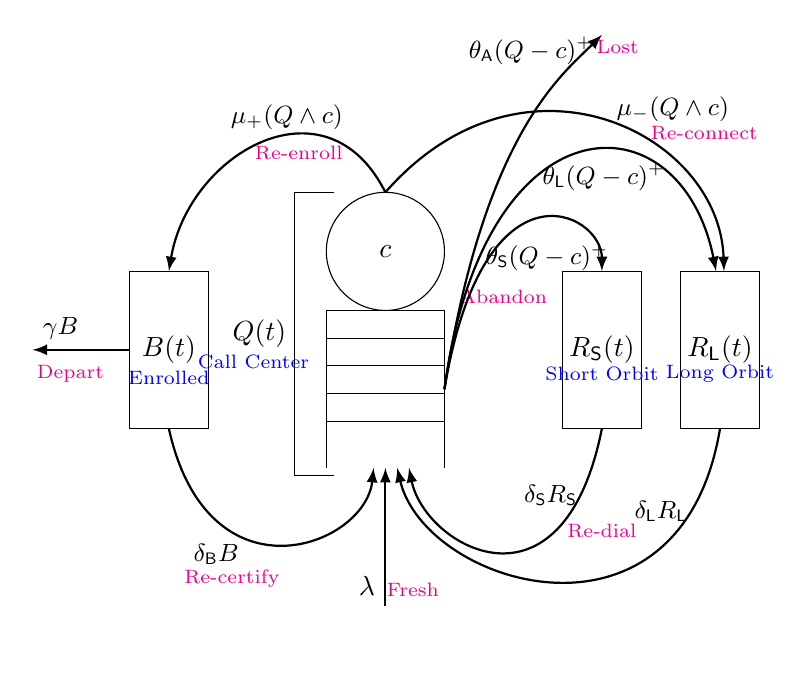
\begin{tikzpicture}[>=latex, rotate=90]

    \draw (-0.1,-0.1) -- ++(0,0.5cm) -- ++(3.6cm,0)  -- ++(0,-0.5cm);
\node[align=center] at (1.35cm,0.925cm) {\scriptsize \textcolor{blue}{Call Center}};
\node[align=center] at (1.7cm,0.85cm) {$Q(t)$};

% the rectangle at the bottom with vertical rules
\draw (0,0) -- ++(2cm,0) -- ++(0,-1.5cm) -- ++(-2cm,0);
\foreach \i in {1,...,4}
  \draw (2cm-\i*10pt,0) -- +(0,-1.5cm);

% the circle
\draw (2.75,-0.75cm) circle [radius=0.75cm];

% the arrows and labels for bottom part
\draw[<-, thick] (0,-0.75) -- +(-50pt,0) node[above left] {$\lambda$};
\node[align=center] at (-1.55cm,-1.1cm) {\scriptsize \textcolor{magenta}{Fresh}};

\node at (2.75,-0.75cm) {$c$};

% the rectangle above with "Enrolled"
\draw (0.5,2.5) -- ++(2cm,0) -- ++(0,-1cm) -- ++(-2cm,0) --++ (0,1cm);
\node[align=center] at (1.5cm,2cm) {$B(t)$};
\node[align=center] at (1.15cm,2cm) {\scriptsize \textcolor{blue}{Enrolled}};
\draw[->, thick] (1.5cm,2.5cm) -- +(0,35pt) node[above right] {\small $\gamma B$};
\node[align=center] at (1.2cm,3.25cm) {\scriptsize \textcolor{magenta}{Depart}};

% the outgoing arch from circle to the right side of the "Enrolled" rectangle
\draw[->, thick] (3.5,-0.75) .. controls (5,0) and (4,1.75) .. (2.5,2);
\node[align=center] at (4.45cm,0.5cm) {\small $\mu_{\mathsf{+}} (Q \wedge c)$};
\node[align=center] at (4cm,0.35cm) {\scriptsize \textcolor{magenta}{Re-enroll}};

\node[align=center] at (2.175cm,-2.25cm) {\scriptsize \textcolor{magenta}{Abandon}};
\draw[->, thick] (1,-1.5) .. controls (4,-2) and (3.25,-3.5) .. (2.5,-3.5);
\node[align=center] at (2.675cm,-2.8cm) {\small $\theta_\mathsf{S} (Q - c)^+$};
\draw[->, thick] (1,-1.5) .. controls (4.75,-2) and (4.75,-4.5) .. (2.5,-4.95);
\node[align=center] at (3.7cm,-3.525cm) {\small $\theta_\mathsf{L} (Q - c)^+$};
\draw[->, thick] (1,-1.5) .. controls (4.25,-2) and (5,-3) .. (5.5,-3.5);
\node[align=center] at (5.3cm,-2.6cm) {\small $\theta_\mathsf{A} (Q - c)^+$};
\node[align=center] at (5.35cm,-3.7cm) {\scriptsize \textcolor{magenta}{Lost}};


\draw[->, thick] (3.5,-0.75) .. controls (5.5,-2.5) and (4.25,-5) .. (2.5,-5.05);
\node[align=center] at (4.55cm,-4.4cm) {\small $\mu_{\mathsf{-}} (Q \wedge c)$};
\node[align=center] at (4.25cm,-4.8cm) {\scriptsize \textcolor{magenta}{Re-connect}};

\draw[->, thick] (0.5,-3.5) .. controls (-2,-3) and (-1,-1.25) .. (0,-1.05);
\node[align=center] at (-0.35cm,-2.85cm) {\small $\delta_\mathsf{S} R_\mathsf{S}$};
\draw[->, thick] (0.5,-5) .. controls (-2.5,-4.5) and (-1.5,-1.25) .. (0,-0.9);
\node[align=center] at (-0.55cm,-4.25cm) {\small $\delta_\mathsf{L} R_\mathsf{L}$};
\node[align=center] at (-0.8cm,-3.5cm) {\scriptsize \textcolor{magenta}{Re-dial}};

\draw[->, thick] (0.5,2) .. controls (-1.75,1.5) and (-1,-0.5) .. (0,-0.6);
\node[align=center] at (-1.1cm,1.4cm) {\small $\delta_\mathsf{B} B$};
\node[align=center] at (-1.4cm,1.2cm) {\scriptsize \textcolor{magenta}{Re-certify}};



\draw (0.5,-3) -- ++(2cm,0) -- ++(0,-1cm) -- ++(-2cm,0) --++ (0,1cm);
\node[align=center] at (1.5cm,-3.5cm) {$R_\mathsf{S}(t)$};
\node[align=center] at (1.2cm,-3.5cm) {\scriptsize \textcolor{blue}{Short Orbit}};

\draw (0.5,-4.5) -- ++(2cm,0) -- ++(0,-1cm) -- ++(-2cm,0) --++ (0,1cm);
\node[align=center] at (1.5cm,-5cm) {$R_\mathsf{L}(t)$};
\node[align=center] at (1.2cm,-5cm) {\scriptsize \textcolor{blue}{Long Orbit}};

\end{tikzpicture}
\vspace{-.3in}
\caption{Process flow diagram of a queueing theoretic model of the SNAP call center.}\label{queueFig}
\end{figure}


\paragraph{Definition of the SNAP call center stochastic model}

%Allow us to now formally define the queueing model.
In a manner closely following \citet{ding2015fluid} but with further details added for the sake of the problem context, let us model the call center as a Markovian service network.  First, let $Q(t)$ be the number of callers either actively speaking to one of the $c \in \mathbb{Z}_+$ agents or waiting for the next available agent at time $t \geq 0$. Let $\lambda > 0$ be the rate of ``fresh'' or exogenous arrivals to the call center for those newly seeking to enroll in benefits. Suppose that each agent completes calls at rate $\mu = \mu_{\mathsf{+}} + \mu_{\mathsf{-}}$ for $\mu_{\mathsf{+}}, \mu_{\mathsf{-}} > 0$, where each completed call has a probability $\mu_{\mathsf{+}}/\mu$ of being {successfully} completed, meaning that the caller will not need to call back in order to complete enrollment and receive benefits, and probability $\mu_{\mathsf{-}}/\mu$ of being unsuccessful, meaning that the caller will need to call back. Let $B(t)$ track the number of successfully enrolled recipients at time $t$. Successfully enrolled recipients will either eventually ``qualify out'' of the system or otherwise need to re-certify. 
%Accordingly, we suppose that  for each recipient in $B(t)$, there is an independent and exponentially distributed time with rate $\delta_\mathsf{B}$ until they will must re-certify and an independent and exponentially distributed time with rate $\gamma$ until they leave the system, and the recipient will follow whichever occurs first. Hence, 
At rate $\delta_\mathsf{B} B(t)$, $B(t)$ will decrease by one with $Q(t)$ simultaneously increasing by one, and at rate $\gamma B(t)$, $B(t)$ will simply be decremented. 
%For callers that complete a call unsuccessfully, we will let $R_\mathsf{L}(t)$ be the number of callers who will eventually call back but after a relatively long time (on average), which we assume to be independently and exponentially distributed with rate $\delta_\mathsf{L}$ for all such callers.

Now, we will suppose that callers waiting for the next available agent each have independently and exponentially patience time with rate $\theta = \theta_\mathsf{A} + \theta_\mathsf{S} + \theta_\mathsf{L} > 0$ for $\theta_\mathsf{A}, \theta_\mathsf{S}, \theta_\mathsf{L} \geq 0$. With probability $\theta_\mathsf{A}/\theta$, the caller will abandon the queue and never call back to re-attempt enrollment. Then, with probability $\theta_\mathsf{S}/\theta$, the caller will hang up but eventually ``re-dial'' or attempt to call back after a (likely) short amount of time. Let $R_\mathsf{S}(t)$ be the number of callers at time $t$ who have left the queue but will soon re-dial, where each re-dial time is independent and exponentially distributed with rate $\delta_\mathsf{S}$. Finally, with probability $\theta_\mathsf{L}/\theta$, a caller will hang up and eventually call back but after a long time like the unsuccessful callers; hence, we count both types of callers among $R_\mathsf{L}(t)$. On aggregate, at rate $\delta_\mathsf{S} R_\mathsf{S}(t)$, $R_\mathsf{S}(t)$ will decrease by one with $Q(t)$ increasing by one, and, likewise, at rate $\delta_\mathsf{L} R_\mathsf{L}(t)$, one caller from $R_\mathsf{L}(t)$ will transition back to $Q(t)$.






In this way, the full model $(Q, B, R_\mathsf{S}, R_\mathsf{L})$ is a multi-station queueing network where the $Q$ station is a $\cdot/M/c$ queue and each of $B$, $R_\mathsf{S}$, and $R_\mathsf{L}$ are $\cdot/M/\infty$ queues. We visualize this queueing network in Figure~\ref{queueFig}. 
Formally, the stochastic process $(Q,B,R_\mathsf{S}, R_\mathsf{L})$ can be constructed through Poisson processes:
\begin{align}
Q(t)
\label{QDef}
&=
Q(0)
+
\Pi_\lambda\left(t\right)
+
\Pi_{\mathsf{B}}\left(\textstyle{\int_0^t} \delta_\mathsf{B} B(s) \mathrm{d}s\right)
+
\Pi_{\mathsf{S}}\left(\textstyle{\int_0^t} \delta_\mathsf{S} R_\mathsf{S}(s) \mathrm{d}s\right)
+
\Pi_{\mathsf{L}}\left(\textstyle{\int_0^t} \delta_\mathsf{L} R_\mathsf{L}(s) \mathrm{d}s \right)
\\
&
\quad
-
\Pi_{\mathsf{Q:A}}\left(\textstyle{\int_0^t} \theta_\mathsf{A} \left(Q(s) - c \right)^+ \mathrm{d}s \right)
-
\Pi_{\mathsf{Q:S}}\left(\textstyle{\int_0^t} \theta_\mathsf{S} \left(Q(s) - c \right)^+ \mathrm{d}s \right)
-
\Pi_{\mathsf{Q:L}}\left(\textstyle{\int_0^t} \theta_\mathsf{L} \left(Q(s) - c \right)^+ \mathrm{d}s \right)
\nonumber
\\
&
\quad
-
\Pi_{\mathsf{Q:+}}\left(\textstyle{\int_0^t} \mu_\mathsf{+}\left(Q(s) \wedge c \right) \mathrm{d}s\right)
-
\Pi_{\mathsf{Q:-}}\left(\textstyle{\int_0^t} \mu_\mathsf{-}\left(Q(s) \wedge c \right) \mathrm{d}s\right)
,
\nonumber
\\
B(t)
\label{BDef}
&=
B(0)
+
\Pi_{\mathsf{Q:+}}\left(\textstyle{\int_0^t} \mu_\mathsf{+}\left(Q(s) \wedge c \right) \mathrm{d}s\right)
-
\Pi_{\mathsf{B}}\left(\textstyle{\int_0^t} \delta_\mathsf{B} B(s) \mathrm{d}s\right)
,
\\
R_\mathsf{S}(t)
\label{RSDef}
&=
R_\mathsf{S}(0)
+
\Pi_{\mathsf{Q:S}}\left(\textstyle{\int_0^t} \theta_\mathsf{S} \left(Q(s) - c \right)^+ \mathrm{d}s \right)
-
\Pi_{\mathsf{S}}\left(\textstyle{\int_0^t} \delta_\mathsf{S} R_\mathsf{S}(s) \mathrm{d}s\right)
,
\\
R_\mathsf{L}(t)
\label{RLDef}
&=
R_\mathsf{L}(0)
+
\Pi_{\mathsf{Q:-}}\left(\textstyle{\int_0^t} \mu_\mathsf{-}\left(Q(s) \wedge c \right) \mathrm{d}s\right)
+
\Pi_{\mathsf{Q:L}}\left(\textstyle{\int_0^t} \theta_\mathsf{L} \left(Q(s) - c \right)^+ \mathrm{d}s \right)
-
\Pi_{\mathsf{L}}\left(\textstyle{\int_0^t} \delta_\mathsf{L} R_\mathsf{L}(s) \mathrm{d}s \right)
.
\end{align}
Here, as in the literature \citep[e.g.,][]{mandelbaum1998strong,pang2007martingale}, we use $\Pi_i(\cdot)$ for $i \in \mathcal{I} = \{\lambda, \mathsf{B}, \mathsf{S}, \mathsf{L}, \mathsf{Q:A}, \mathsf{Q:S}, \mathsf{Q:L}, \mathsf{Q:+}, \mathsf{Q:-}\}$ are mutually independent unit-rate Poisson processes. We assume that $Q(0)$, $B(0)$, $R_\mathsf{S}(0)$, and $R_\mathsf{L}(0)$ are known initial conditions.



\paragraph{Model interpretability via Poisson thinning and superposition} 
Because the queueing network model is composed from a collection of Poisson processes, we can leverage well-known probabilistic properties to further interpret its transitions.
The transition rates can equivalently be interpreted through standard Poisson thinning: abandoning callers enter the lost, short-redial, and long-redial paths in proportions $\theta_A/\theta$, $\theta_S/\theta$, and $\theta_L/\theta$, while completed calls succeed with probability $\mu_+/\mu$ and otherwise enter the reconnect orbit. See \Cref{apx-addl-discussion} for more explanation. 




\subsection{Fluid model}

As a simpler companion to the stochastic queueing model, let us also define the deterministic \emph{fluid model} $(q,b,r_\mathsf{S}, r_\mathsf{L})$ through the following system of ordinary differential equations (ODEs):
\begin{align}
&
\dot{q}(t)
\label{qDef}
=
\lambda
+
\delta_\mathsf{B} b(t)
+
\delta_\mathsf{S} r_\mathsf{S}(t)
+
\delta_\mathsf{L} r_\mathsf{L}(t)
-
\theta (q(t) - c)^+
-
\mu (q(t) \wedge c)
,
&&
\dot{b}(t)
%\label{bDef}
=
\mu_\mathsf{+} (q(t) \wedge c)
-
(\delta_\mathsf{B} + \gamma) b(t)
,
\\
&
\dot{r}_\mathsf{L}(t)
\label{rlDef}
=
\mu_\mathsf{-} (q(t) \wedge c)
+
\theta_\mathsf{L} (q(t) - c)^+
-
\delta_\mathsf{L} r_\mathsf{L}(t)
,
&&
\dot{r}_\mathsf{S}(t)
%\label{rsDef}
=
\theta_\mathsf{S} (q(t) - c)^+
-
\delta_\mathsf{S} r_\mathsf{S}(t)
.
\end{align}
As one may recognize by comparison to Figure~\ref{queueFig}, the dynamics of these ODEs align with the overall flow of the queueing model. However, the fluid model is deterministic, unlike the stochastic queueing model, suggesting that the fluid model could be a good first-order approximation for the queue. There is a clean intuition for that approximation: Imagine the call center queue as a physical system, where callers actually arrive to process through the network as visualized in Figure~\ref{queueFig}. Now, imagine those customers as arriving faster and faster, but also proportionally shrinking smaller and smaller, so that they move through the various services and orbits faster and faster as well. As this shrinking and speeding goes to the extreme, the queueing network would look like a continuous flow of callers in and out of the stations of the queue, where the random times between arrivals, abandonments, completed calls, re-dials, re-connects, and re-enrolls would be replaced by fluid at the same rates. Moreover, following intuition granted by the law of large numbers, the stochastic fluctuations brought by those random arrival, abandonment, and service times should eventually be dominated by the sheer scale of the growing and accelerating system.

This intuition can be formalized: the fluid model indeed arises out of a functional strong law of large numbers (FSLLN) limit of the queueing model, and we now formalize this connection in Proposition~\ref{fluidLimit}.

\begin{proposition}\label{fluidLimit}
For $n \geq 0$, let $\left(Q^{(n)}, B^{(n)}, R_\mathsf{S}^{(n)}, R_\mathsf{L}^{(n)}\right)$ be the queueing network model of~\eqref{QDef} through~\eqref{RLDef} alternately defined with external arrival rate $\lambda n$ and number of servers $c n$. Then, given that
\begin{align}
\lim_{n \to \infty}
\left(\frac{1}{n}Q^{(n)}(0), \frac{1}{n}B^{(n)}(0), \frac{1}{n}R_\mathsf{S}^{(n)}(0), \frac{1}{n}R_\mathsf{L}^{(n)}(0)\right)
\longrightarrow
\left(q^0, b^0, r_\mathsf{S}^0, r_\mathsf{L}^0\right)
,
\end{align}
the fluid limit of the scaled stochastic process converges to the deterministic system,
\begin{align}
\lim_{n \to \infty}
\left(\frac{1}{n}Q^{(n)}(t), \frac{1}{n}B^{(n)}(t), \frac{1}{n}R_\mathsf{S}^{(n)}(t), \frac{1}{n}R_\mathsf{L}^{(n)}(t)\right)
\stackrel{\mathsf{a.s.}}{\longrightarrow}
\left(q(t), b(t), r_\mathsf{S}(t), r_\mathsf{L}(t)\right)
,
\end{align}
uniformly on compact sets, where $\left(q(t), b(t), r_\mathsf{S}(t), r_\mathsf{L}(t)\right)$ is the unique solution to the system of equations in~\eqref{qDef} through~\eqref{rlDef} with initial condition $\left(q(0), b(0), r_\mathsf{S}(0), r_\mathsf{L}(0)\right) = \left(q^0, b^0, r_\mathsf{S}^0, r_\mathsf{L}^0\right)$.
\end{proposition}
\begin{proof}
This fluid limit can be readily obtained from prior functional strong law results from the literature; for instance, the proof of this limit follows immediately from theorem 2.2 of \citet{mandelbaum1998strong}.%, where section 5 therein provides a relevant specific application of that general FSLLN
result. \rev{Alternatively, one can also obtains this fluid limit via the standard ``recipe'' of \citet{ethier2009markov}, as \citet{ding2015fluid} does excellently. %and the predecessor model in \citet{ding2015fluid} offers an excellent example of how to apply those tools in this type of setting.
}
\end{proof}


From this combination of intuition and rigorous connection, fluid models are very commonly used to study queueing models in a simplified manner that grants tractability but still captures the heart of the modeling context.\footnote{Critically, let us note that the solutions to the fluid model equations need not exactly match the underlying means of the stochastic model, especially for queues with abandonment \citep[e.g.,][]{daw2019new}. Nevertheless, for large systems with many arrivals and many servers (as in our motivating context), the stochastic model is typically close enough to the fluid approximation for its first-order insights to be both valid and valuable, as implied by Proposition~\ref{fluidLimit}.} 
These benefits are particularly evident when studying the steady state of the system, in which the system of ODEs simplify to a system of linear equations.
By setting the equations in~\eqref{qDef} and~\eqref{rlDef} each to 0 and solving for an equilibrium solution, which we denote $(\bar q, \bar b, \bar r_\mathsf{S}, \bar r_\mathsf{L})$, this fluid model admits a first-order approximation for the system's steady-state means:
\begin{align}
\bar q
&=
\left(
c \wedge \left(1 + \frac{\delta_\mathsf{B}}{\gamma}\right)\frac{\lambda}{\mu_\mathsf{+}}
\right)
+
\frac{1}{\theta_\mathsf{A}}
\left(
\lambda - \frac{\gamma c \mu_{\mathsf{+}}}{\gamma + \delta_\mathsf{B}} 
\right)^+
,
\qquad
&&
\bar b 
=
\left(
\frac{\lambda}{\gamma}
\wedge
\frac{c\mu_{\mathsf{+}}}{\gamma + \delta_\mathsf{B}}
\right)
,
\\
\bar r_\mathsf{L}
&=
\left(
\frac{c\mu_{\mathsf{-}}}{\delta_\mathsf{L}}
\wedge
\left(
1 + \frac{\delta_\mathsf{B}}{\gamma}
\right)
\frac{\lambda \mu_{\mathsf{-}}}{\delta_\mathsf{L}\mu_{\mathsf{+}}}
\right)
+
\frac{\theta_\mathsf{L}}{\delta_\mathsf{L} \theta_\mathsf{A}}
\left(
\lambda - \frac{\gamma c \mu_{\mathsf{+}}}{\gamma + \delta_\mathsf{B}} 
\right)^+
,
\qquad
&&
\bar r_\mathsf{S}
=
\frac{\theta_\mathsf{S}}{\delta_\mathsf{S} \theta_\mathsf{A}}
\left(
\lambda - \frac{\gamma c \mu_{\mathsf{+}}}{\gamma + \delta_\mathsf{B}} 
\right)^+
.
\end{align}

\paragraph{Distinguishing arrival rates in the fluid model} By comparison to the \emph{fresh} arrival rate, $\lambda$, which only counts callers that are newly seeking benefits, the overall rate of arrivals to the system will also include re-dialing callers and current benefit recipients seeking to re-enroll. Because the total arrival rate is both an important quantity in its own right and more readily observed in data, let us formalize it in notation. Specifically, in the fluid model, let 
$\hat \lambda(t) 
= 
\lambda
+
\delta_\mathsf{B} b(t)
+
\delta_\mathsf{S} r_\mathsf{S}(t)
+
\delta_\mathsf{L} r_\mathsf{L}(t)$ 
denote the \rev{\emph{total arrival rate}} to the system at time $t$, and, without the $t$ argument, let 
$\hat \lambda
= 
\lambda
+
\delta_\mathsf{B} \bar{b}
+
\delta_\mathsf{S} \bar{r}_\mathsf{S}
+
\delta_\mathsf{L} \bar{r}_\mathsf{L}$ 
be the total arrival rate for the fluid model in steady-state. 

Furthermore, in studying the caller experience, it will also be of interest to focus on the volume of arrivals that includes the re-dialing and re-enrolling orbits but excludes the customers that renege from the queue before connecting to an agent. To be able to compute values such as the average waiting time among callers that do not abandon, let us define $\tilde{\lambda}(t) = \hat\lambda(t) - \theta(q(t) - c)^+$ as the \rev{\emph{effective arrival rate}, i.e. the total arrival rate at time $t$ less abandonments}, and we again let the argument-less $\tilde \lambda$ denote \rev{the effective arrival rate in steady-state}.


\paragraph{Simplifications in the overloaded regime.} When the system is overloaded, i.e. $q(t) \geq c$, then we can simplify the branching logic so that $(q(t) - c)^+ = q(t) -c$ and $(q(t) \wedge c)=c$. Moreover, in  steady-state, the overloaded regime can be easily characterized, and it yields simple expressions for the four model quantities.



%\paragraph{Equations expressed in readily interpretable metrics}

%\tr{can solve for the fresh arrival rate, $\lambda$, in terms of the observed total arrival rate, $\hat \lambda$}
%\begin{align}
%\lambda
%&=
%\frac{\theta_\mathsf{A}}{\theta} 
%\left(\hat \lambda - c\mu\right)^+
%+
%\frac{\gamma}{\gamma + \delta_\mathsf{B}}
%\cdot
%\frac{\mu_{\mathsf{+}}}{\mu}
%\left(
%\hat \lambda \wedge c \mu
%\right)
%,
%\end{align}
%\tr{and each of these terms can be interpreted: $\hat p_{\mathsf{Ab}} := \theta_\mathsf{A}/\theta$ is the probability that a caller who abandons before being answered will never call back, $\hat p_{\mathsf{Ret}} = \delta_\mathsf{B} / (\gamma + \delta_\mathsf{B})$ is the retention probability of current recipients of benefits, and $\hat p_{\mathsf{Suc}} = \mu_{\mathsf{+}} / \mu$ is the fraction of completed calls that successfully resolved the caller's issue. Then, recalling that $c$ is the number of servers and $1/\mu$ is the average call duration, the fresh arrival rate can be re-expressed as}



\begin{corollary}\label{overCor}
The overloaded regime, $\bar{q} \geq c$, occurs as the equilibrium fluid model solution if and only if $\lambda \geq {\gamma c \mu_{\mathsf{+}}}/({\gamma + \delta_\mathsf{B}})$, which equivalently occurs if and only if $\hat{\lambda} \geq c\mu$. In this case, the steady-state solutions simplify to
\begin{align}
\bar{q}
&= \frac{1}{\theta_{\mathsf{A}}}
\left(\lambda - \frac{\gamma c\mu_{\mathsf{+}} }{\gamma + \delta_{\mathsf{B}}}\right) 
+ c, \qquad 
\bar{b}
= \frac{c\,\mu_{\mathsf{+}}}{\gamma + \delta_{\mathsf{B}}}, 
\qquad 
\bar{r}_S = \frac{\theta_{\mathsf{S}}}{\theta_{\mathsf{A}} \delta_{\mathsf{S}}}
\left(\lambda - \frac{\gamma c\mu_{\mathsf{+}} }{\gamma + \delta_{\mathsf{B}}}\right) ,
\qquad 
\bar{r}_L= \frac{c\mu_{\mathsf{-}}}{\delta_{\mathsf{L}}}
+ \frac{\theta_{\mathsf{L}}}{\delta_{\mathsf{L}} \theta_{\mathsf{A}}}
\left(\lambda - \frac{\gamma c\mu_{\mathsf{+}} }{\gamma + \delta_{\mathsf{B}}}\right) .\label{eqn-steady-state-simplified}
\end{align}
\end{corollary}

%\tr{state largely work with overloaded fluid model from here forward -- parsimonious model is the simplest first step to being exploring the SNAP call center data and the impacts of possible changes to the system}

In the remainder of the paper, we will largely focus on the steady-state fluid model and assume it to be in the overloaded regime. This parsimonious approximation offers the simplest first step to derive insights from the \emph{Holmes v. Knodell} data and assess the impacts of possible changes to the SNAP call center system. %While there are many interesting details and important questions that can be asked of the random model or in a transient state, this parsimonious fluid approximation offers the simplest first step to start exploring the \emph{Holmes v. Knodell} data and assess the impacts of possible changes to the SNAP call center system. 
The overloaded assumption is well-justified, here and more broadly, since system-level stresses motivate us to study the problem in the first place.
%Furthermore, both in this specific context and in general call center analyses, we feel the overloaded assumption is not without justification, as it is such system-level stresses that motivate us to study the problem in the first place.
 
\section{Data and Model Fitting}

In this section, we illustrate how to connect our model parameters to call center data in general, and we discuss how we do so for Missouri DSS' call centers via the aggregated data released in court documents. %First, we discuss the available call center data and information, based on the court documents. Then, we overview how model parameters relate to the available data. We fit the parameters that we can to data; some are not informed by available data, so we consider a range of reasonable values based on the domain. 


% \begin{itemize}
%     \item Average wait time (including those who abandon) 
%     \item Average time to answer (wait time of people who actually make it through, excluding abandonments) 
% \end{itemize}

\textbf{Fitting model parameters in general: }

\textit{Simple parameter matching from observable metrics: }The eleven parameters used by the queueing model
%-- $\lambda$, $\gamma$, $\delta_\mathsf{B}$, $\delta_\mathsf{L}$, $\delta_\mathsf{S}$, $\theta_\mathsf{A}$, $\theta_\mathsf{L}$, $\theta_\mathsf{S}$, $\mu_{\mathsf{+}}$, $\mu_{\mathsf{-}}$, $c$ -- 
may not actually all be readily identifiable in practice. For instance, the model uses $\lambda$, the rate of \emph{fresh} arrivals only, as a parameter, whereas $\hat \lambda$, the total rate of all arrivals, is likely what is recorded operationally either by hand or by typical call center management software. Rather, disentangling $\lambda$ from $\hat \lambda$ is actually a possible benefit of the model. 

% For a broad strokes approach to divining model parameters from real-world contexts, let us first consider what quantities should be observable in practice and then connect them to the steady-state fluid approximation, which we assume to be operating in the overloaded regime. 
Let us consider what quantities should be observable in practice and connect them to the (overloaded) steady-state fluid approximation.\footnote{If fine-grained data on arrival times and call durations is available, more rigorous techniques like maximum likelihood estimation can deliver high fidelity parameter estimation. But since the fluid model is itself already a deterministic approximation to the queueing model's stochastic approximation of reality, these back-of-the-envelope calculations can be used to guide calibration of the fluid model from aggregated data.} %rewriting for short 
% First, %as we have said above, 
% we would expect that call center management knows or can measure the total arrival rate, $\hat \lambda$. %, to be known to the management of the call center. 
% Similarly, the service rate, $\mu$, or the more recognizable $1/\mu$ the average call duration is readily observable.\footnote{This service time \textit{excludes} waiting and its calculation \textit{excludes} any callers who abandon before being connected to an agent.}
% although it may be more recognizable as $1/\mu$ being the average call duration, excluding waiting and not counting any callers who abandon before being connected to an agent. 
Several inputs are directly observable or administratively specified: total arrivals $\hat{\lambda}$, staffing $c$, average handling time $1/\mu$\footnote{This service time \textit{excludes} waiting and its calculation \textit{excludes} any callers who abandon before being connected to an agent.}, the re-certification interval $1/\delta_\mathsf{B}$, $\bar{q}$ and $\bar{b}$, the average number of present callers (including both waiting and in service), and benefits retention, which pins down $\gamma$ through $\delta_\mathsf{B}/(\gamma+\delta_\mathsf{B})$. 
% We will take as known the staffing level, $c$, 
% % as known. We furthermore expect that the 
% the time from benefit enrollment to re-certification, which gives $\delta_\mathsf{B}$ via $1/\delta_\mathsf{B}$ as the time until re-certification begins,
% % and we likewise expect the 
% and benefits retention to be known, which  gives $\gamma$ via $\delta_\mathsf{B}/(\gamma + \delta_\mathsf{B})$ as the retention rate. We expect $\bar{q}$ and $\bar{b}$, the average number of present callers (including both waiting and in service), $\bar{q}$, and number of recipients presently enrolled in a benefits program like SNAP, are taken as known. %For instance, the fluid model views the average number of callers who abandon before being answered per unit of time as $\theta(\bar{q}-c)^+$, and, taking both $\bar{q}$ and $c$ as known, this delivers $\theta$.
%a first-order performance metric for call center management, and the number of recipients presently enrolled in a  benefits program like SNAP, which is modeled as $\bar{b}$, is similarly a first-order quantity for the management of the public service program. We will thus take $\bar{q}$ and $\bar{b}$ as known and work back towards the underlying parameters of the model. For instance, the fluid model views the average number of callers who abandon before being answered per unit of time as $\theta(\bar{q}-c)^+$, and, taking both $\bar{q}$ and $c$ as known, this delivers $\theta$.


Assuming that the system is in the overloaded regime, we can take the above assumptions of observable quantities within the equilibrium fluid model and the definitions of $\hat \lambda$, $\theta$, and $\mu$ to provide a system of equations for the remaining model quantities. We do so now, and we underline the unknown terms in each equation for emphasis:
\begin{align*}
\begin{alignedat}{4}
0&=\underline{\lambda}+\delta_\mathsf{B}\bar b
+\underline{\delta_\mathsf{S}}\underline{\bar r_\mathsf{S}}
+\underline{\delta_\mathsf{L}}\underline{\bar r_\mathsf{L}}
-\theta(\bar q-c)-c\mu,
&\qquad
0&=c\underline{\mu_+}-(\gamma+\delta_\mathsf{B})\bar b,
&\qquad
0&=\underline{\theta_\mathsf{S}}(\bar q-c)
-\underline{\delta_\mathsf{S}}\underline{\bar r_\mathsf{S}},
&\qquad
0&=c\underline{\mu_-}
+\underline{\theta_\mathsf{L}}(\bar q-c)
-\underline{\delta_\mathsf{L}}\underline{\bar r_\mathsf{L}},
\\
\hat\lambda
&=\underline{\lambda}+\delta_\mathsf{B}\bar b
+\underline{\delta_\mathsf{S}}\underline{\bar r_\mathsf{S}}
+\underline{\delta_\mathsf{L}}\underline{\bar r_\mathsf{L}},
&\qquad
\theta&=\underline{\theta_\mathsf{A}}
+\underline{\theta_\mathsf{L}}
+\underline{\theta_\mathsf{S}},
&\qquad
\mu&=\underline{\mu_-}+\underline{\mu_+}.
\end{alignedat}
\end{align*}
% \begin{align}
% 0
% &=
% \underline{\lambda} + \delta_\mathsf{B} \bar{b} + \underline{\delta_\mathsf{S}} \underline{\bar{r}_\mathsf{S}} + \underline{\delta_\mathsf{L}} \underline{\bar{r}_\mathsf{L}} - \theta (\bar{q} - c) - c \mu
% ,
% \qquad
% &&
% 0 
% =
% c \underline{\mu_+} - (\gamma + \delta_\mathsf{B})\bar{b}
% ,
% \nonumber
% \\
% 0
% &=
% \underline{\theta_\mathsf{S}} (\bar{q} - c)  - \underline{\delta_\mathsf{S}} \underline{\bar{r}_\mathsf{S}}
% ,
% \qquad
% &&
% 0
% =
% c \underline{\mu_-}  + \underline{\theta_\mathsf{L}} (\bar{q} - c)  - \underline{\delta_\mathsf{L}} \underline{\bar{r}_\mathsf{L}}
% ,
% \\
% \hat \lambda
% &=
% \underline{\lambda} + \delta_\mathsf{B} \bar{b} + \underline{\delta_\mathsf{S}} \underline{\bar{r}_\mathsf{S}} + \underline{\delta_\mathsf{L}} \underline{\bar{r}_\mathsf{L}}
% ,
% \qquad
% &&
% \theta
% =
% \underline{\theta_\mathsf{A}} + \underline{\theta_\mathsf{L}} + \underline{\theta_\mathsf{S}}
% ,
% \qquad
% &&&
% \mu 
% = 
% \underline{\mu_{-}} + \underline{\mu_{+}}
% .
% \nonumber
% \end{align}
As written, this system has seven equations and ten unknowns. Hence, we need more information to solve for the missing values, albeit perhaps not as much as it might seem. First, consider $\delta_\mathsf{S}$, $\delta_\mathsf{L}$, $\bar{r}_\mathsf{S}$, and $\bar{r}_\mathsf{L}$. Several approaches can quickly reduce these four to just two missing values. For instance, one can estimate $\delta_\mathsf{S}$ and $\delta_\mathsf{L}$ from time-series data, or work directly with the \emph{volume} of returning callers per unit of time, say $\bar{v}_\mathsf{S} = \delta_\mathsf{S} \bar{r}_\mathsf{S}$ and $\bar{v}_\mathsf{L} = \delta_\mathsf{L} \bar{r}_\mathsf{L}$, which preserves our ability to evaluate key performance metrics. 
%\footnote{For instance, in our data set, we use an auto-regressive time series analysis on the daily call volumes to suggest values for $\delta_\mathsf{S}$ and $\delta_\mathsf{L}$, which then simply leaves $\bar{r}_\mathsf{S}$ and $r_\mathsf{L}$ as unknown. On the other hand, if such data analysis is not possible, though, one can simply abstract away from viewing the $\delta$ individual rate and $\bar{r}$ average number in orbit separately to a single metric for the \emph{volume} of returning callers per unit of time, say $\bar{v}_\mathsf{S} = \delta_\mathsf{S} \bar{r}_\mathsf{S}$ and $\bar{v}_\mathsf{L} = \delta_\mathsf{L} \bar{r}_\mathsf{L}$. Even though this abstraction would mean that we would lose some amount of visibility into the model overall, it would not compromise our access to evaluating key performance metrics: the degree of procedural denials and the volume of endogenous congestion can still be evaluated in this setting.} 
Taking such reduction for granted, we are left with seven linear equations and eight unknowns. We can %turn to the abandonment dynamics to 
pin down this final degree of freedom %. In practice, remaining ambiguity can be handled 
in one of three ways: use domain knowledge to fix the short- versus long-redial split, simplify to a single redial orbit ($\theta_\mathsf{S}=0$), or sweep over plausible abandonment/redial parameters and compare the implied metrics to auxiliary data. We take the last approach in our analysis.
% In the best case, in practice, there may be some domain knowledge that delivers these quantities, e.g., knowing the fraction of re-dialing callers that do so sooner rather than later, %which is modeled as 
% $\theta_\mathsf{S}/(\theta_\mathsf{S} + \delta_\mathsf{L})$. At the other extreme, without domain knowledge, %if little is known about the abandonment or re-dialing dynamics, 
% one could accordingly reduce the model complexity by setting $\theta_\mathsf{S} = 0$, which would acknowledge the ambiguity and simplify the model to have only one orbit (i.e., $\bar{r}_\mathsf{S} = 0$ if $\theta_\mathsf{S} = 0$). Finally, if neither of those two extremes match the context, one could simply sweep over possible values of $\theta_\mathsf{A}$, and triangulate the resulting solution against additional data; %to some additional data or other outside information to determine the most reasonable option;
% we take this sweeping approach in our own analysis.



% Let us emphasize that the above is certainly not the only approach to calibrate the model parameters, and, moreover, given fine-grained data on arrival times and call durations, proper statistical estimation techniques like maximum likelihood estimation can deliver high fidelity parameters for the queueing models. Nevertheless, given that the fluid model is merely a deterministic approximation of the stochastic queueing model, which itself is at best an approximation of reality, these back-of-the-envelope calculations can be sufficient to leverage the fluid model to assess the qualitative impacts of broad-strokes changes to the call center system.

\textbf{Fitting Parameters to the Holmes vs. Knodell Data:}

\rev{\textit{Dataset description: }
We downloaded the Holmes vs. Knodell court documents from the PACER database, which include extensive reports (typically monthly, weekly or daily). %on arrival rates, call center staffing, and various other performance metrics like average handling time and average wait time. 
% ``Exhibit 87'' contains a series of spreadsheets with aggregated call center information which informs our parameter fitting analysis. 
We primarily analyze data from ``Exhibit 87'''s daily aggregated reports from four different call centers, varying in size, spanning 9/29/2021-12/29/2023, though not all call centers report information for the whole time period. (Some of these call centers are centralized CSCs that handle calls for other DSS programs such as Medicaid.) %Recorded data covers 9/29/2021-12/29/2023, though not all call centers report information for the entirety of this time period. 
We observe information about: call volume (number of incoming calls, calls answered successfully, calls abandoned); wait time in queue (before successful connection or abandonment, ASA [average speed to answer] before successful connection, AHT [average handling time] spent by agent on a call's duration); and staffing.
% We observe the number of ``Offered'' calls (total number of incoming calls), ``Answered calls'' (total successfully answered by an agent), ``Abandon'' (total number of calls that hung up while waiting in the queue), ``Avg Wait'' (time spent waiting in the queue before successful connection or abandonment), ``ASA (Average Speed of Answer)'' (time a call is expected to wait in queue before being answered by an agent), ``AHT" (time an agent spends on an answered call), ``Average Abandon Time'' (time spent in queue before hanging up), ``Staffing'' (number of available staff), and ``Calls/Person". 
Average daily call volume per call center is around $(700, 2500, 3100, 6800)$ with average abandonment fractions $(2.5\%, 58\%, 57\%, 57\%)$. The large call volume justifies our fluid approximation. Given the heterogeneity in call center volumes and staffing, we later fit parameters separately to each call center. See \Cref{apx-callcenterdata} for more details.}

\textit{Parametrizing the Queueing Model from Aggregated Call Center Data: }We now discuss how we fit parameters specifically for the aggregated call center and arrival data for court documents from \textit{Holmes v. Knodell}, see \Cref{apx-callcenterdata} for more detail. %Notably, court documents provide only \textit{aggregated} arrival data information, which we describe in more detail in \Cref{apx-callcenterdata}. 
% Nonetheless, we can fit important parameters to data to calibrate the model. 
We parametrize everything in terms of the number of minutes a call center is open in a day, $\rev{MMin}=540 \text{min}=9 \text{ hours}$; the call centers are open on weekdays. In our model, some \textit{operational} parameters such as the total arrival rate $\hat{\lambda}$, staffing levels $c$, and average handling time (AHT) are directly observed in the call-center data. % Thus we can directly set $\hat\lambda, c$, and the sum  $1/AHT = \mu_{\mathsf{+}}+\mu_{\mathsf{-}}$ from data. 
To reduce parameter dimensionality, we fix a proportion $p_+\in[0,1]$ of completed calls that result in completed re/-enrollments, hence $\mu_{\mathsf{+}} = p_+ \left( \frac{\rev{MMin}}{AHT} \right).$ %Some policy and process parameters, such as the recertification hazard $\delta_{\mathsf{B}}$, the short- and long-orbit re-dial rates $\delta_{\mathsf{S}}$ and $\delta_{\mathsf{L}}$, and the enrollment share $p_+$, reflect program rules and eligibility process structure. Therefore to set 
We set $\delta_{\mathsf{B}},\delta_{\mathsf{S}},\delta_{\mathsf{L}},p_+$ by using a combination of program design, domain knowledge, and time series analysis. \rev{\textit{Program design} determines $\delta_{\mathsf{B}} = 1/128.5$ since per SNAP eligibility guidelines, the recertification period is 6 calendar months $\approx$ 128.5 model (call center) days. %We use domain context to set the parameter value for $\delta_{\mathsf{S}}$, the re-dial short orbit rate, which describes the rate that which re-dialers in the short orbit call back. 
\textit{Domain knowledge} sets $\delta_{\mathsf{S}}=3$, corresponding to a typical callback time of $3$ hours; this is a behavioral assumption about within-day callback behavior.} %Therefore the daily rate is $\delta_{\mathsf{S}} = 9 \text{ hours} / 3 \text{ hours} = 1 \text{ day } / (1/3 \text{ day}) = 3.$ 
%This reflects within-day callback attempts, for example trying again because the line was busy earlier. 
The remaining behavioral parameters governing abandonment and re-dial behavior, $(\lambda,\theta_{\mathsf{A}},\theta_{\mathsf{S}},\theta_{\mathsf{L}})$, namely the fresh arrival rate $\lambda$ and rates of total abandonment $\theta_A$, short/long orbit abandonment $\theta_S,\theta_L$, are not directly observed in our aggregated data.\footnote{From data, we only have measures of aggregated abandonment percentages (typically daily or weekly).}




% \paragraph{Parameters where the data is uninformative.}
% We have some parameters where the data is uninformative. 



% The parameters $\theta_{\mathsf{A}}, \theta_{\mathsf{S}}, \theta_{\mathsf{L}}$ describe the total abandonment rate (never re-dials), abandonment of those who leave the queue but call back shortly and therefore enter the short orbit, and abandonment of those who leave the queue enter the long orbit to call back on a longer timeframe, respectively. From data, we have measures of abandonment percentages (typically daily or weekly). 
\textit{Derived metrics and an operational dashboard: }The steady-state approximation allows us to derive \textit{model-based estimates} of performance metrics. The model results best inform \textit{relative comparisons} as to how changes in call center design \textit{increase or decrease key metrics}. We introduce the resulting \textit{model-based performance metrics}, which use the approximated steady state values and include: average wait time  ($\bar{w} = (\bar{q}-c)^+ / \hat \lambda$), which includes abandonments),  average speed to answer ($\tilde{w} = (\bar{q}-c)^+ /\tilde \lambda$), which does not include abandonments), abandonment fraction ($1 - \frac{\tilde{\lambda}}{\hat\lambda}$), total lost abandonment ($\theta_{\mathsf{A}} (\bar{q}-c)^+$), and endogenous congestion from re-dials ($ \delta_{\mathsf{S}} \bar r_{\mathsf{S}} + \delta_{\mathsf{L}} \bar r_{\mathsf{L}}$). 

%\begin{itemize}
    %\item Average wait times $\bar{w} = (\bar{q}-c)^+ / \hat \lambda$ (including abandonments) 
    %\item "Average speed to answer" $\tilde{w} = (\bar{q}-c)^+ /\tilde \lambda$ 
    %\item Abandonment rate = $1 - \frac{\tilde{\lambda}}{\hat\lambda}$
    %\item Total abandonment - a lower bound on procedural denials, $\theta_{\mathsf{A}} (\bar{q}-c)^+ $
%\item Inflow from rebound calls $ \delta_{\mathsf{S}} r_{\mathsf{S}} + \delta_{\mathsf{L}} r_{\mathsf{L}}$
%\end{itemize}


We can interpret the metric of lost calls, $\theta_{\mathsf{A}} (\bar{q}-c)^+,$ those who completely leave the system, as a metric related to procedural denials. The fluid model is not sharp enough to estimate whether a single caller would get through in $30$ days, so \rev{our total abandonment metric is a policy-relevant lower bound on procedural denials. Of the other quantities, wait times directly affect customer experience and are key metrics in essentially any call center.}
\rev{Other relevant values include utilization $U = {\tilde{\lambda}}/{c \mu} ,$ which measures the ratio of the \emph{effective} arrival rate to service capacity and also captures the average fraction of service providers that are busy, and the 
implied utilization
    $IU  ={\hat\lambda}/{c\mu}$, which is a common adaptation of the utilization metric to \emph{all arrivals} that also measures overload (i.e., $IU$ can exceed 1 whereas $U \leq 1$).\footnote{\rev{By consequence of Corollary~\ref{overCor}, we can observe that, in the overloaded regime, $U=1$ and $IU \geq 1$.}}}

We develop an analytics dashboard where stakeholders could perturb system parameters to examine impacts on these performance metrics, see \Cref{fig:dashboard} in the Appendix for a screenshot.\footnote{The (anonymized version of) the dashboard is publicly available at \url{https://call-center-simulator-production.up.railway.app}.}

\textit{Robustly fitting $\lambda$ over a range of plausible $\theta_{\mathsf{A}}, \theta_{\mathsf{S}}, \theta_{\mathsf{L}}$: } 
Since the finer-grained behavioral parameters $\theta_{\mathsf{A}}, \theta_{\mathsf{S}}, \theta_{\mathsf{L}}$ are uninformed from data, we fit a single fresh arrival rate parameter $\lambda$ that recovers wait times well over a \textit{potential range of plausible values of $\theta_{\mathsf{A}}, \theta_{\mathsf{S}}, \theta_{\mathsf{L}}$}. We assess how the derived wait times $\bar{w},\tilde{w}$ compare to \textit{observed} wait times (including abandonment) and speed to answer (excluding abandonment). 
There are four different call centers in Exhibit 87. We group them by call volume and average handling time, two in a 20 minute AHT category and two in a 40 minute AHT category. We calculate the median average wait time and median average speed to answer. 
% Since $\theta_{\mathsf{A}},\theta_{\mathsf{S}},\theta_{\mathsf{L}}$ are not identified, we sweep over a range of \textit{reasonable} values. 
We sweep over a range of \textit{reasonable} $\theta_{\mathsf{A}},\theta_{\mathsf{S}},\theta_{\mathsf{L}}$; we fix the sum of rates $\theta_{\mathsf{A}}+\theta_{\mathsf{S}}+\theta_{\mathsf{L}}=10$ or $54$ (corresponding to $54$ or $10$ minute abandonment, respectively) and vary the relative weight of $\theta_{\mathsf{A}},\theta_{\mathsf{S}},\theta_{\mathsf{L}}$. Finally, we robustly fit $\lambda$ by minimizing the mean average deviation (averaging over $\theta$ parameter vector values) of median wait times.
%We therefore consider a variety of scenarios with different proportions of $\theta_{\mathsf{A}},\theta_{\mathsf{S}},\theta_{\mathsf{L}}$ respectively. 

%For all of these similarly plausible combinations of parameters, our goal is to see that the simulation's derived metrics approximately align with observed wait times. Since exactly matching observed metrics would likely result in overfitting the non-identified parameters, our overall goal is to check that these similarly plausible parameters result in wait times within, say, an order of magnitude of observed average wait times. 


  \begin{table}[t!]
  \centering
    \caption{Descriptive statistics on observed metrics for call centers (CC), and
  best-fit lambda values and MAD for each call center. Staffing and arriving
  calls are daily metrics.}\label{tab:parameter-fitting}

  \small
  \setlength{\tabcolsep}{4pt}
  \begin{tabular}{@{}cccccccc@{}}
  \toprule
  CC & c (staffing) & AHT (min) & Wait (min) & ASA (min) & observed $
  \hat{\lambda}$ & best-fit $\lambda$ & Best MAD ($\bar{w}$, $\tilde{w}$) \\
  \midrule
  1 & 32.5 & 20.8 & 4.4 & 4.1 & 228.0 & 145.4 & (1.2, 1.9) \\
  2 & 52.0 & 21.9 & 38.8 & 117.8 & 2931.5 & 623.3 & (2.9, 27.0) \\
  3 & 72.0 & 44.2 & 45.5 & 87.6 & 2396.5 & 700.1 & (11.6, 20.8) \\
  4 & 51.0 & 44.8 & 1.8 & 1.8 & 712.0 & 164.8 & (1.1, 1.6) \\
  \bottomrule
  \end{tabular}

  \vspace{-0.1in}
  \end{table}
% \begin{table}[t!]
% \centering
% \begin{tabular}{|c|c|c|c|c|c|c|c|}
% \hline
% CC & c (staffing) & AHT (min) &  Wait (min) & ASA (min) & observed $\hat{\lambda}$ & best-fit $\lambda$ & Best MAD ($\bar{w}$, $\tilde{w}$) \\
% \hline
% 1 & 32.5 & 20.8 & 4.4 & 4.1 & 228.0 & 145.4 & (1.2, 1.9) \\
% \hline
% 2 & 52.0 & 21.9 & 38.8 & 117.8 & 2931.5 & 623.3 & (2.9, 27.0) \\
% \hline
% 3 & 72.0 & 44.2 & 45.5 & 87.6 & 2396.5 & 700.1 & (11.6, 20.8) \\
% \hline
% 4 & 51.0 & 44.8 & 1.8 & 1.8 & 712.0 & 164.8 & (1.1, 1.6) \\
% \hline
% \end{tabular}
% \caption{Descriptive statistics on observed metrics for call centers (CC), and best-fit lambda values and MAD for each call center. Staffing and arriving calls are daily metrics. }
% \vspace{-0.1in}
% \label{tab:parameter-fitting}
% \end{table}

\textit{Observed metrics and fitted parameters: }This table summarizes the key metrics for the four call centers, separating the empirically observed data from the fitted model parameters. The columns from ``c (staffing)'' through ``observed $\hat{\lambda}$'' represent the direct operational measurements. All time metrics are shown in decimal minutes. Specifically, ``Average Wait Time (min)'' and ``ASA (min)" correspond to the observed values for $\bar{w}$ and $\tilde{w}$, respectively, while ``observed $\hat{\lambda}$'' is the total arrival rate including re-dials. In contrast, the ``best-fit $\lambda$'' is a fitted parameter, representing the optimized robust rate of fresh arrivals derived from the model. The final column, ``Best MAD ($\bar{w}$, $\tilde{w}$)'', quantifies model fit with the Mean Absolute Deviation between model predictions and the ``Average Wait Time'' and ``ASA Time'', respectively. 





\section{Evaluating system design changes}

% Before running policy changes: 
% - ``refit" lambda to match lambda hat 
%\subsection{Analysis}

\paragraph{Analytical results for operational changes in the general fluid model}

We begin by leveraging closed-form solutions for steady-state expressions for the performance metrics to analyze \textit{how} different potential operational changes affect system performance in the overloaded regime. Specifically, we now analyze six key steady-state performance metrics: the procedural denial rate ($\mathrm{PD} = \theta_A (\bar q - c)$), the mean number of waiting callers ($\bar{q} - c$), the mean waiting time ($\bar w = (\bar q - c) / \hat \lambda$), the average speed to answer ($\tilde w = (\bar q - c) / \tilde \lambda$), the endogenous congestion from re-dials ($\mathrm{EC}_\mathsf{R} = \delta_\mathsf{S} \bar r_\mathsf{S} + \delta_\mathsf{L} \bar r_\mathsf{L}$), and the endogenous congestion from re-certification ($\mathrm{EC}_\mathsf{B} = \delta_\mathsf{B} \bar b$).   For each quantity, we evaluate its dependence on four model parameters that could reasonably be subject to managerial control or operational design: the staffing level ($c$), the frequency of re-certification ($\delta_\mathsf{B}$), the individual service rate ($\mu$), and the fraction of successful calls (which we denote $p_+ = \mu_+ / \mu$, with $\mu$ assumed to be held fixed).\footnote{Though endogenous congestion from re-dials is undoubtedly bad for the system, the service agents, and the callers themselves, endogenous congestion from re-certifications might actually be considered at least somewhat good: it is a sign that people are successfully receiving SNAP benefits.} 

Intuitively, while $c$ may be expensive to increase, it may be relatively easy to re-design the eligibility interview process to be either faster (increase $\mu$) or more likely to result in certification (increase $p_+$), and, likewise, structural policy changes could increase the re-certification period (decrease $\delta_\mathsf{B}$). Here, we leverage the fluid model to offer insight of how these prospective changes may relate to one another.
In the interest of space, the exact expressions of the partial derivatives of each performance metric with respect to each operational parameter are left for the appendix (see Propositions~\ref{dPDprop} through~\ref{dECBprop}), and here we simply highlight their takeaways in a series of corollary results. %We begin with the following review of the  directional dependence of each performance metric on each operational parameter.

First, we establish that any of the prospective changes will yield intuitive directional improvements in the procedural denial rate, the waiting time, the average speed to answer, and the number waiting. 

% \begin{corollary}
% In the overloaded regime, 
% the procedural denial rate, mean waiting time, average speed to answer, and mean number waiting are each decreasing with $c$, $\mu$, and $p_+$ and increasing with $\delta_\mathsf{B}$.
% \end{corollary}

% Then, we similarly find that the volume of arriving callers seeking to re-certify will increase with higher staffing, faster service, better conversion rates, or shorter re-certification periods.

% \begin{corollary}
% In the overloaded regime,
% the endogenous congestion from re-certifications is increasing with each of the operational parameters. 
% \end{corollary}

% On the other orbit, the endogenous congestion from re-dials decreases with better conversion or shorter re-certification periods, but, interestingly, it could either increase or decrease with higher staffing or faster service.


% \begin{corollary}
% In the overloaded regime,
% the endogenous congestion from re-dials is increasing with $\delta_\mathsf{B}$ and decreasing with $p_+$. However, the endogenous congestion from re-dials increases with $c$ and $\mu$ if
% % \begin{align}
% $\theta_\mathsf{A} (1 - p_+)(\gamma + \delta_\mathsf{B})
% > 
% p_+  \gamma c (\theta_\mathsf{S} + \theta_\mathsf{L})$
% ,
% % \end{align}
% and otherwise it is non-increasing with $c$ and $\mu$.
% \end{corollary}


\begin{corollary}[Directional comparative statics]
In the overloaded regime, the procedural denial rate, mean waiting time, average speed to answer, and mean number waiting are each decreasing in $c$, $\mu$, and $p_+$ and increasing in $\delta_\mathsf{B}$. Endogenous congestion from re-certifications is increasing in each operational parameter. Endogenous congestion from re-dials is increasing in $\delta_\mathsf{B}$ and decreasing in $p_+$; its dependence on $c$ and $\mu$ is ambiguous, increasing with $c$ and $\mu$ if $\theta_\mathsf{A}(1-p_+)(\gamma+\delta_\mathsf{B})>p_+\gamma c(\theta_\mathsf{S}+\theta_\mathsf{L})$, and otherwise non-increasing in $c$ and $\mu$.
\end{corollary}

The main access-oriented metrics improve under candidate operational changes: increasing staffing, increasing service speed, increasing the fraction of successful calls, or lengthening the re-certification period. However, endogenous congestion from redials behaves differently: it decreases with better conversion or shorter re-certification periods, but, interestingly, it could either increase or decrease with higher staffing or faster service. 

%Re-certification congestion rises when more callers are successfully enrolled or retained, while re-dial congestion falls with higher successful-completion rates or longer re-certification periods but can move either way with added staffing or faster service. 

To compare magnitudes rather than only signs, we next consider elasticities of the performance metrics with respect to the operational parameters. For a metric $y$ and parameter $x$, the local elasticity is $(x/y)\partial y/\partial x$. First, we find that changes to staffing level, service rate, and probability of success all yield the same respective elasticity for the procedural denial rate, number waiting, and endogenous congestion from re-certifications. For relative magnitudes, the key result is that staffing and service-speed improvements have identical proportional effects in the overloaded regime.

\begin{corollary}[Elasticity equivalences]
For each of PD, $\bar q-c$, and ECB, the elasticity is the same across $c$, $\mu$, and $p_+$. For each of $\bar w$, $\tilde w$, and ECR, the elasticity is the same across $c$ and $\mu$ (but different from the previous elasticity).
\end{corollary}

% \begin{corollary}
% For each of $\mathrm{PD}$, $\bar q - c$, and $\mathrm{EC}_\mathsf{B}$, the elasticity is the same across $c$, $\mu$, and $p_+$ in the overloaded regime. 
% \end{corollary}


% \begin{corollary}
% For each of $\bar w$, $\tilde w$, and $\mathrm{EC}_\mathsf{R}$, the elasticity is the same across $c$ and $\mu$ in the overloaded regime.
% \end{corollary}

Then, for the waiting time, speed to answer, and endogenous congestion from re-dials, changes to the staffing level and to the service rate again yield equivalent elasticities, but they need not be the same as that of the success probability.
These corollaries together show that changes to $c$ and $\mu$ have the same respective impact for each of the six performance metrics, suggesting that they have equivalent operational impacts despite their likely quite different costs. 

% \paragraph{Metrics matter: subtleties in different definitions.} [[Subtle differences in definitions of metrics matter. E.g. average speed to answer vs. average wait time. Reference court discussions about different definitions of metrics. Reference SSA discussions about different sorts of metrics]] [[implications of metric definition, i.e. individual-centric wait time measures per individual vs. total waiting load. Increases in arrivals also increase the averaging base, moderating policy impacts. ]]
\paragraph{Comparison of our endogenous-congestion-aware queueing model to generic Erlang-A staffing guidance}
In \Cref{tab:compact_staffing_benchmark}, we compare our model to staffing guidance from naive application of the standard Erlang-A model. Using the Erlang-A model to guide counterfactual staffing decisions is \textit{overly optimistic} and \emph{fundamentally under-staffed} since an abandoning customer leaves the system forever in the Erlang-A model, and therefore the phenomenon of abandonment actually lowers wait times overall. However, our proposed model with re-dials accurately represents the endogenous congestion where an abandoning caller today can actually increase congestion in the future when they re-dial or re-connect. Therefore, its requisite staffing prescriptions increase significantly beyond that of the Erlang-A model. In fact, in applying both models to the four call centers within the \emph{Holmes v. Knodell} data and computing staffing levels necessary for each to achieve standard performance metric targets, we find that the Erlang-A yields as large as a 84\% shortfall of the staffing prescribed from our endogenous-congestion-aware model's guidance. The largest discrepancies are driven by call centers where fitting Erlang-A to observed arrivals cannot fit observed wait times well, further demonstrating that Erlang-A's assumptions are unsuitable for redials in social service delivery.
  \begin{table}[htbp]
  \centering
  \caption{Our model vs. Erlang A. Entries
  in the target columns are required staffing counts to achieve that target. Shortfall is
  $(\mathrm{our\ model}-\mathrm{Erlang\ A})/\mathrm{our\ model}$. The
  abandonment target is the lost/abandoned share in our model $(1-\tilde \lambda /  \hat \lambda)$ and Erlang A's
  abandonment probability. The last column is Erlang A's absolute relative error
  in fitted average wait, $|\widehat{\bar w}_{EA}-\bar w|/\bar w$.}
  \label{tab:compact_staffing_benchmark}
  \begin{tabular}{lc ccc ccc c}
  \toprule
  && \multicolumn{3}{c}{Average wait $<1$ min} & \multicolumn{3}{c}{Abandonment
  $<10\%$} & \multicolumn{1}{c}{Erlang A $\bar w$ error} \\
  \cline{3-5}\cline{6-8}\cline{9-9}
  CC & $c$ & Our model & Erlang A & Shortfall & Our model &
  Erlang A & Shortfall & $|\Delta \bar w|/\bar w$ \\
  \hline
  1 & 32.5 & 52 & 13 & 75.0\% & 52 & 8 & 84.6\% & 100.0\% \\
  2 & 52 & 194 & 125 & 35.6\% & 174 & 107 & 38.5\% & 107.1\% \\
  3 & 72 & 217 & 203 & 6.5\% & 195 & 177 & 9.2\% & 22.1\% \\
  4 & 51 & 58 & 58 & 0.0\% & 58 & 56 & 3.4\% & 5.4\% \\
  \bottomrule
  \end{tabular}
\vspace{-0.1in}
  \end{table}





\paragraph{Possible improvements: staffing vs.~system design efficiency curves based on \emph{Holmes v. Knodell} data}

\begin{figure}[t!]
    \centering
    \subcaptionbox{Staffing-AHT curves, wait times; decreases in AHT\label{fig:wait_time-aht}}{%
\includegraphics[width=0.24\textwidth]{Figs/wait_time_aht_20260113_151200.png}%
    }
    \hfill
    \subcaptionbox{Staffing-AHT curves, procedural denials\label{fig:denials-aht}}{%
        \includegraphics[width=0.24\textwidth]{Figs/denials_vs_aht_20260113_151214.png}%
    }
        \subcaptionbox{Wait time vs. recertification length, $\delta_{\mathsf{B}}$\label{fig-wait-recert}}{%
\includegraphics[width=0.24\textwidth]{Figs/wait_recerts.png}%
    }
    \hfill
    \subcaptionbox{Daily procedural denials vs recertification period (changes in $\delta_{\mathsf{B}}$). \label{fig:denials-recert}}{%
        \includegraphics[width=0.26\textwidth]{Figs/denials_recerts.png}%
    }
    \vspace{-.2in}
    \caption{Performance metrics vs staffing levels for different potential changes in call center system design.}
    \label{fig:staffing-curves}
\end{figure}

% Policy changes (describe analytically first):
% \begin{itemize}
%     \item Change recertification rate: Change both the rates for $\gamma$ and $\delta_{\mathsf{B}}$ (1 year to 2 year)
%     \item Average handling time: both $\mu_{\mathsf{+}}$, $\mu_{\mathsf{-}}$ increase, but proportionally
%     \item Higher effectiveness of interviews: ratio of $\mu_{\mathsf{-}}$ to $\mu_{\mathsf{+}}$
% \end{itemize} 

While the prior analysis highlights the impact of potential system design changes one at a time, in \Cref{fig:staffing-curves} we leverage the model fitted to \textit{Holmes v. Knodell} call center data to explore the joint efficiency of \textit{simultaneous} improvements in staffing and other system design changes. Importantly, our richer model enables also assessing the impact of these other policy design and service delivery changes on performance metrics. \Cref{fig:staffing-curves} illustrates in \textit{AHT vs. staffing curves} how performance improvements in wait times and procedural denials depend on interactions between system design and staffing (on the x-axis) improvements. We generate these figures for one of the call centers (\#2); results for other call centers are qualitatively similar, hence omitted. We use a $\theta$ parameter vector $(\theta_{\mathsf{A}}, \theta_{\mathsf{S}},\theta_{\mathsf{L}}) =(4,3,3)$ --- although different values of $\theta_{\mathsf{A}}, \theta_{\mathsf{S}},\theta_{\mathsf{L}}$ result in different absolute magnitude estimates for wait times, all of our commentary depends on \textit{relative} orderings that remain the same, and procedural denial metrics depend only on $\theta_{\mathsf{A}}.$ \Cref{fig:wait_time-aht,fig:denials-aht} compare average wait-time and procedural denials on the y-axis as staffing changes, for different improvements in \textit{average handling time (AHT)}; each value of the AHT generates a different staffing curve.\footnote{System design changes that reduce AHT might include recent interest in AI chatbots, automated responses, increased training for staffing, or self-service options --- these could handle simple questions more briefly or redirect callers to new self-service channels.} In \Cref{fig:wait_time-aht} we see wait times decrease sharply at low staffing levels, with diminishing returns at higher staffing. Meanwhile, procedural denials (under our model --- total abandonment) decrease linearly in staffing but decreasing AHT increases the rate of enrolled individuals, and hence further improves the \textit{efficiency} of staffing improvements (slope of decrease in denials). Jointly considering system design improvements and staffing increases can \textit{increase the performance improvements} under practically limited additional staffing resources. Conversely, \textit{without} making changes in call center design and service process, it can take an unrealistically large number of additional staff to reduce wait times or procedural denials to acceptable levels. \rev{To concretely illustrate practical insights, recall that DSS estimated that it needed at least 150 additional staff to reduce wait times below 2 minutes. Our quantitative models estimate that to achieve this \textit{without} any additional staff, DSS must reduce handling time by 75\%, or lengthen recertification periods to 1 year. With just $50$ extra staff, it suffices to reduce handling time by 50\%, and so on.} %, but under our assumption of completed enrollments scaling proportionally in the average handling rate (service rate), $\mu_{+} =\rho\left(\frac{MMin }{A H T}\right),$ decreasing AHT increases the rate of enrolled individuals, and hence the efficiency of staffing improvements (slope of decrease in denials). 

In \Cref{fig-wait-recert,fig:denials-recert} we investigate the same types of staffing curves if we consider \textit{longer re-certification cycles}, from 6 months to 1 or 2 years. While longer re-certification cycles don't improve wait-time efficiency as much as improving service time does, longer recertification periods continue to improve procedural denial efficiency. The moderated joint impact on \textit{wait times} reflects an interesting distinction between \textit{per-individual} performance metrics like average wait time per caller vs. \textit{absolute magnitude} performance metrics like total abandonment/procedural denials. Longer re-certification periods maintain enrollment loads but \textit{reduce} arrival rates, therefore averaging waits over a \textit{smaller} total load and attenuating the improvements from higher throughput. Interventions that reduce {congestion and arrivals} have similar \textit{self-attenuating} effects on rate-based rather than absolute metrics.  



\rev{\textit{Broader practical context of potential interventions: }%Our quantitative model enables comparing the relative efficacy of different interventions by mapping their service improvements into changes in system inputs. %Different interventions also have different \textit{institutional feasibility}: changing re-certification length for everyone is a matter of federal policy (or obtaining waivers for specific categories) but could increase payments to individuals who may become ineligible. 
Different interventions have different institutional constraints: longer recertification periods may require federal policy changes, while reductions in handling time require service redesign that preserves accuracy and quality. 
% Shortening handling times without harming quality of service or accuracy may require strategic service re-design, like introducing self-service options. Of course, there is also great interest in using AI to improve call center performance for SNAP, just as there is elsewhere in customer service; but AI tools could degrade service quality via errors. 
% Practice-based discussions often involve other strategies beyond our 
Practitioners realize improvements via more specific tactics beyond our abstract discussions here \citep{nj-call-centers}. 
%\footnote{\rev{For example, New Jersey made drastic improvements through a variety of tactics, including re-designing call menus based on frequently requested options and adding self-service \citep{nj-call-centers}.}} 
While there is also general interest in AI, it cannot completely replace interview provision (due to merit pay designations on who can complete what work), but would be deployed in narrow ways to improve processes.
Our model translates such heterogeneous interventions into key operational inputs, such as arrivals, handling time, and completion rates.
% (Indeed, budget requests indicate that Missouri DSS requested \$4 million for an AI chatbot \citep{aolRecordsShow}.) 
% Nonetheless, AI deployments face fundamental limits due to regulations requiring that ``merit pay'' employees handle sensitive data and casework, so that . %While using technology can help, there ultimately are limits as there are federal regulations dictating that some sensitive/confidental casework tasks need to be conducted by ``merit pay" employees, and hence cannot be freely outsourced. 
% Whether system improvements come from AI or careful adjustments to practical system design, any improvements to call center performance must pass through key system parameters like arrivals, handling time, and others. 
}

\section{\rev{Conclusion}}

\rev{In this work, we introduced a performance evaluation framework for queueing analysis in social services, fit model parameters to call center data from \textit{Holmes v. Knodell}, and derived analytical and practical quantified insights on substitutable improvement levers. 
Since there are no unilateral performance requirements for backlogs in social services, the ultimate goal of our performance evaluation framework is to enable agencies themselves (e.g. via a dashboard) to explore different performance improvement options ex-ante, transparently, and flexibly. %Different proposed improvements in call center management can be mapped abstractly to our key model inputs and parameters in order to evaluate relative trade-offs in the system performance vs. potential difficulty of implementing different changes. 
}


\rev{\textit{Model limitations and future research: } 
The performance metrics we have studied here are of first-order importance operationally, but they are also merely results of the fluid model, which is itself a first-order approximation of the queueing model. Moreover, there are other queueing-theoretic quantities of at least equal practical importance
%, such as the variance of the endogenously-driven arrival rate of callers or a caller's probability of being connected within $n$ call attempts,
that cannot be analyzed by a fluid model. For instance, redials are a clear problem in the motivating \emph{Holmes v. Knodell} setting, both in terms of the load on the system from the endogenous congestion and in terms of the administrative burden on individuals. 
%As we have previously discussed, the case documents make clear that the plaintiffs made many call attempts over short time periods to try to get through the overloaded system \cite{holmesKnodell2024}. 
A truly probabilistic analysis of the model would allow us to study the distribution of a caller's requisite number of attempts before connection, thus offering insight for how this  emergent arbitrariness might be ameliorated.
}

% \clearpage

%\paragraph{Acknowledgments}

%We thank Issa Kohler-Hausmann, Dan Ho, Elizabeth Edwards, Jamie L. Rodriguez, Katie Deabler, Jae Yeon Kim, and the EAAMO Working Group on Inequality for discussions. 

% \paragraph{Endmatter - Generative AI Usage Statement
% }
% We leveraged generative AI (Sonnet 4.5) to help in modifying code, building the Streamlit dashboard web app from simulation code, generating LaTeX tables. 

\paragraph{Ethical Considerations Statement}

The goal of our work was to improve social impact and equity by carefully studying technical systems (queueing) that currently mediate access to crucial benefits, are currently failing, and lack accurate guidance in light of unique characteristics of social service delivery. Our work could have unintended impacts --- after all, we focus on introducing and analyzing performance metrics, but there's always Goodhart's law, ``When a measure becomes a target, it ceases to be a good measure". Indeed, we refer to prior instances of potential gaming or misreporting/misrepresentation of queueing performance metrics, like with efforts to improve the SSA waits \citep{warren}. We try to mitigate potential unintended consequences by highlighting some distinctions between different performance metrics and focusing on a general performance evaluation framework, rather than any single metric in particular. 
%% The next two lines define the bibliography style to be used, and
%% the bibliography file.
\bibliographystyle{ACM-Reference-Format}
\bibliography{FAccT-template/snap-refs.bib} 

\clearpage

%%
%% If your work has an appendix, this is the place to put it.
\appendix

\section{Background}

\paragraph{Additional discussion on related work}
For the most part, the so-called \textit{civic tech} community is the technical practitioner community focused on digital delivery of services and provision of government benefits. Books and grey literature document the challenges of technical deployment and product design in government settings \citep{pahlka2023recoding}. Recent works in the FAccT community have also explored the interface of benefits technology and equity. \citet{escher2020exposing} audits benefits calculators, which are a category of online tools that distill the government's original, remarkably complex eligibility forms into more UX-friendly, shorter screeners. Such benefits screeners, however, might provide accessibility and reduce frictions at the expense of \textit{accuracy} in eligibility determinations. \citet{jo2025ai} conducts an interview study to assess SNAP applicants' interactions with potential LLM-based chatbots, studying the interface between trust issues in AI and potential improvements in administrative burdens. \citet{koenecke2023popular} find that an efficient advertising budget for GetCalfresh, which streamlines enrollment in California's CalFresh (SNAP), resulted in low takeup among Hispanic individuals: The authors conduct a survey and find general public support for \textit{equitable} advertising budget allocations with higher spending on advertising aimed at harder-to-reach populations.

\paragraph{Additional background on benefits tech}

Government digital infrastructure faces several structural challenges that prevent rapid iteration and performance evaluation feedback loops: contracting out implementation to large vendors in cumbersome public procurement processes, larger "waterfall" and non-"agile" contracts that introduce inflexible system design, limited in-house technical capacity, and vendor opacity due to trade secrets protection. For example, when Missouri announced intentions to deploy a new version of Medicaid home-based care determination algorithms, policy analysts and analysts had to band together to bring potentially affected individuals together to audit potential impacts on care. Benefits technological infrastructure (hence called "benefits tech" for short) falls in this category - it must interface with proprietary data mainframes and is often contracted out via public procurement, where few firms have the capacity to work with government legacy systems, and so there is little market pressure to compete on performance. They found that the updated algorithm would remove 66\% of affected individuals from crucial home nurse care as well as potential syntax errors in the algorithm \citep{noauthor_missouri_nodate}. Without this community audit, such deployments would have introduced harmful erroneous determinations silently --- it would be three more years before Missouri contracted a consultant to analyze the impacts of an updated algorithm. 

The call center system design and deployment in this setting is somewhat different from prior major benefits tech infrastructure projects, in that call center technology is in principle well-developed in the commercial sector. But, call center design and operations are usually contracted out, as Missouri DSS did to Genesys, a major provider. Designing call center systems and queues is a specialized skill with little guidance from FNS as to performance standards and unlikely in-house expertise in social services. 
\clearpage
\section{Dashboard}

\begin{figure}
    \centering
    \includegraphics[width=\linewidth]{Figs/call-center-dashboard-.jpg}
    \caption{Screenshot of call center dashboard}
    \label{fig:dashboard}
\end{figure}
\clearpage

\section{Additional explanation}\label{apx-addl-discussion}


\paragraph{Additional explanation of Poisson thinning}
For example, consider the dynamics  of the number of presently enrolled  recipients. Intuitively, the next decrease to $B(t)$ will be either a departure via attrition from the benefits system or a return to the call center to re-certify. Because of the memoryless property of the underlying exponential random variables between events in Poisson processes, we can view this as a ``race'' between two exponentially distributed ``clocks'' -- one for attrition and one for re-certification.\footnote{Moreover, because of the thinning property of the Poisson itself, we can granularize this same interpretation to the level of each currently enrolled individual: for each current benefit recipient, there is a $\mathsf{Exp}(\gamma)$ clock for the time to potential attrition and a $\mathsf{Exp}(\delta_\mathsf{B})$ clock for the time to potential re-certification, and whichever clock rings first will be what happens next.} Hence, by these same properties, there is a $\gamma/(\gamma + \delta_\mathsf{B})$  probability that the recipient departs via attrition and a $\delta_\mathsf{B}/(\gamma + \delta_\mathsf{B})$ probability that they instead call to re-certify.
Similar interpretations abound throughout the model: an abandoning caller enters the short orbit with probability $\theta_\mathsf{S}/(\theta_\mathsf{A} + \theta_\mathsf{S} + \theta_\mathsf{L})$, a concluding caller enters the long orbit with probability $\mu_-/(\mu_+ + \mu_-)$, and each of the $(Q(t) \wedge c)$ ongoing calls are equally likely to be the next to conclude.
\section{Call center arrival data }\label{apx-sec-call-center-ts-analysis}


\section*{Data Dictionary: Call Center Performance Metrics (Offered, Answered, Abandoned)}\label{apx-callcenterdata}

\begin{table}[h!]
    \centering
    \caption{Key Metrics from Offered, Answered, Abandoned Data Files}
    \label{tab:data_dictionary_offered_answered}
    \begin{tabular}{|l|p{10cm}|}
        \hline
        \textbf{Field Name} & \textbf{Description} \\
        \hline
        \texttt{Offered} & Total number of incoming calls presented to the call system or queue. \\
        \hline
        \texttt{Answered} & Total number of calls successfully answered by an agent. \\
        \hline
        \texttt{Abandon} & Total number of calls that hung up while waiting in the queue before being answered. \\
        \hline
        \texttt{Abandon \%} & Percentage of calls that abandoned (\texttt{Abandon} / \texttt{Offered}). \\
        \hline
        \texttt{Avg Wait} / \texttt{Average Wait} & Average time a caller spent waiting in the queue before being connected to an agent or abandoning. \\
        \hline
        \texttt{ASA (Average Speed of Answer)} & The average time a call is expected to wait in the queue before being answered by an agent. \\
        \hline
        \texttt{AHT (Average Handle Time)} & The average amount of time an agent spends on an answered call (including talk time and wrap-up work). \\
        \hline
        \texttt{Average Abandon Time} & The average amount of time abandoned calls spent in the queue before the caller hung up. \\
        \hline
        \texttt{Staffing} & The total number of staff members scheduled or logged in to handle calls during the interval. \\
        \hline
        \texttt{Calls/Person} & A staff productivity metric, calculated as calls handled per staff member. \\
        \hline
    \end{tabular}
\end{table}

\subsection{Parameter fitting based on data}

%\tr{hold}
%\begin{align}
%\lambda
%&=
%\hat{p}_{\mathsf{Ab}}
%\left(\hat \lambda - c\mu\right)^+
%+
%\left(1 - \hat{p}_\mathsf{Ret}\right)\hat{p}_\mathsf{Suc}
%\left(\hat \lambda \wedge c\mu\right)
%\end{align}

\paragraph{Parameters directly observed in data} 

From the data, we directly observe some of the parameters. 


% From data, we observe $\hat\lambda$, the total arrival rate of calls. This includes not only the fresh arrivals $\lambda$, i.e. calls originating not from prior cases, but also incoming calls from recertifications $(\delta_{\mathrm{B}} b(t))$, re-dials from prior abandoned or re-connected calls entering the short orbit $(\delta_{\mathrm{S}} r_{\mathrm{S}})$, and re-dials from prior calls entering the long orbit, $(\delta_{\mathrm{L}} r_{\mathrm{L}}(t))$. The observed arrival rate is therefore:
    % , fresh arrival rate of calls (from individuals who have not abandoned or re-dialed from a prior call) 
%    $$\hat \lambda = \lambda+\delta_{\mathrm{B}} b(t)+\delta_{\mathrm{S}} r_{\mathrm{S}}(t)+\delta_{\mathrm{L}} r_{\mathrm{L}}(t)$$

%    We separately define $\tilde{\lambda},$ comprising arrivals that do not abandon and therefore persist through the queue. 

%    $$\tilde{\lambda} = \hat\lambda - (\theta_{\mathsf{A}} + \theta_{\mathsf{S}} + \theta_{\mathsf{L}})*(\bar{Q} - c)^+
%$$
Recall that we have defined $\hat\lambda$ as the total arrival rate of calls, which we observe directly from data. This includes not only the fresh arrivals $\lambda$, i.e. calls originating not from prior cases, but also incoming calls from recertifications $(\delta_{\mathrm{B}} \bar{b})$, re-dials from prior abandoned or re-connected calls entering the short orbit $(\delta_{\mathrm{S}} \bar{r}_{\mathrm{S}})$, and re-dials from prior calls entering the long orbit, $(\delta_{\mathrm{L}} \bar{r}_{\mathrm{L}})$. 

From data, we also directly observe staffing levels, $c,$ for each call center -- we take averages. From SNAP eligibility guidelines, we fix the recertification period is at 6 months (calendar days) $\approx$ 128.5 model (call center) days (since it’s only
open weekdays). This fixes the parameter $\delta_{\mathsf{B}} = 1/128.5$.

The wait time data includes Average Handling Time ($AHT$), 
%\todo{clarify exactly what this refers to} 
and therefore the completion rate of calls, $1/AHT$. Our model further distinguishes service completions into those that complete enrollment ($\mu_{\mathsf{+}}$) vs. those that require a re-connection/re-dial ($\mu_{\mathsf{-}}$). Therefore, completion rates $1/AHT$ are only informative of the sum of these enrollment/re-dial flows:
    $$
  \mu_{\mathsf{+}} + \mu_{\mathsf{-}} = \frac{\rev{MMin}}{AHT} $$
  To reduce parameter dimensionality, we fix a proportion $\rho\in[0,1]$ of completed calls that result in completed re/-enrollments, hence $\mu_{\mathsf{+}} = \rho \left( \frac{\rev{MMin}}{AHT} \right).$ Although $\rho$ is not observed in this data, it may be in other settings, or otherwise informed by the domain. 
% \begin{itemize}
% % \item $MMin=540 \text{min}=9 \text{ hours}$, model minutes: We parametrize everything in terms of the number of minutes a call center is open in a day. 
% %     \item From data, we observe $\hat\lambda$, the total arrival rate of calls. 

% %     This includes arrivals from separate flows as distinguished in our model, including 
% %     $\lambda$, fresh arrival rate of calls (from individuals who have not abandoned or re-dialed from a prior call) 
% %     $$\hat \lambda = \lambda+\delta_{\mathrm{B}} b(t)+\delta_{\mathrm{S}} r_{\mathrm{S}}(t)+\delta_{\mathrm{L}} r_{\mathrm{L}}(t)$$

% %     We separately define $\tilde{\lambda},$ comprising arrivals that do not abandon and therefore persist through the queue. 

% %     $$\tilde{\lambda} = \hat\lambda - (\theta_{\mathsf{A}} + \theta_{\mathsf{S}} + \theta_{\mathsf{L}})*(\bar{Q} - c)^+
% % $$
%     % \item $c$ staffing levels
%     % \item Average Handling Time ($AHT$), \todo{clarify exactly what this refers to}.  The completion rate of calls is $1/AHT$. 
    
    
%   \item We fix a proportion $\rho\in[0,1]$ of completed calls that result in completed re/-enrollments, hence $\mu_{\mathsf{+}} = \rho \left( \frac{MMin}{AHT} \right) $
%   \item The recertification period is fixed at 6 months (calendar days) $\approx 128.5$ model (call center) days (since it's only open weekdays). This fixes the parameter $\delta_{\mathsf{B}} = 1/128.5$
% \end{itemize}

% Deduced parameters: 
% \begin{itemize}
%     \item    $\delta_{\mathsf{S}}$ is the re-dial rate of the re-dial short orbit: given that someone is going to call back in a short timeframe, what is the rate that they call back? 

%     We set $\delta_{\mathsf{S}}$ to reflect a typical callback time of $3$ hours. Therefore the daily rate is $\delta_{\mathsf{S}} = 9 \text{ hours} / 3 \text{ hours} = 1 \text{ day } / (1/3 \text{ day}) = 3.$ This reflects within-day callback attempts, for example trying again because the line was busy earlier. 
%     \item 
% \end{itemize}

\paragraph{Parametrizing  $\delta_{\mathsf{L}}$ from the call center arrival data.}
 The re-dial rate of the long orbit is $\delta_{\mathsf{L}}$, which governs the rate at which re-dials occur from the long orbit (longer timeframe of calling back, for example to obtain and confirm additional verifications). %We use time-series analysis to inform our choice of $\delta_{\mathsf{L}}$, where  we generally find \textit{long-range} dependences on the order of $7-9$ model days, in addition to shorter $1-2$ model day dependences. 
We fit vector-autoregressive regression (VAR) time-series models to the call center offered and abandoned time series data (adjusting for day-of-week fixed effects). In summary, the empirical time-series analysis surfaces dependence in call center volume (offered and abandoned calls) that operates both over the short-term (dependence on prior 1-2 days) and longer-range dependencies (7-9 days). We therefore set $\delta_{\mathsf{L}} = 1/9$. This is consistent with domain discussion about SNAP interviews and how they often require follow-up due to  interview questions that surface or clarify additional documentation needs. %This provides additional supportive evidence for a short- and long-orbit model, in addition to the domain knowledge about document follow-ups.

\subsection{Call center arrival rate analysis}\label{apx-callcenterarrival-ts}


\begin{table}[htb]
\centering
\caption{Call Center Statistics}
\label{tab:call_center_stats}
\begin{tabular}{ccccccc}
\hline
\textbf{Call Center} & \textbf{Mean Offered} & \textbf{Std } & \textbf{Mean Answered} & \textbf{Std } & \textbf{Mean Abandoned} & \textbf{Std } \\
\hline
2 & 3120.06 & 2573.98 & 1229.37 & 1026.57 & 1788.04 & 1872.56 \\
3 & 2555.30 & 891.27 & 882.08 & 281.89 & 1500.85 & 1020.05 \\
4 & 717.15 & 211.77 & 699.21 & 210.99 & 17.88 & 22.54 \\
5 & 6829.01 & 1943.26 & 2729.42 & 866.85 & 3880.46 & 2054.77 \\
\hline
\end{tabular}
\end{table}


% Sum of daily offered calls: 13,221

\paragraph{Periodicity}
We start with one call center, the second in pages 37-87 of exhibit 87. 
As expected, there are day of week effects in calls offered and abandoned. Call volume is the highest on Monday, and decreases over the week (for both offered and abandoned calls). 
We adjust for day of week effects by fitting outcomes to a linear model of just day-of-week effects, subtract off the predictions based on just day-of-week and add back the grand mean. 

Next we fit a vector autoregressive model to the call center time-series data of offered and abandoned calls, separately for each call center. For ease of interpretation, we don’t difference the data, although a Dickey-Fuller test finds only the abandoned calls time series is stationary. 

We use 10 lags in the time series analysis. Note that abandoned calls is a proportion of offered calls of the day, and so naturally tracks offered calls. 

To summarize the time series dependence patterns: Both the volume of offered and abandoned calls track 1) recent, past 1-2 days of offered and abandoned calls and 2) mid-longer range dependencies, like 7-10 days prior. The number of offered calls has a significant coefficient on lagged offered calls for at least 7 out of the first 9 lags, i.e. persistence of call volume (but not necessarily abandoned calls). 

The dependence on prior abandonment is intermittent. Overall, abandonment depends more on prior abandonment than the number of offered calls does. But, we also find occasional statistically significant coefficients on long-range (7-9 day) abandonment. 


\begin{table}[htbp]
\centering
\caption{Call center 2}
\label{table-callcenter-1}
\small
\renewcommand{\arraystretch}{0.9}
\setlength{\tabcolsep}{4pt}

\begin{tabularx}{0.92\linewidth}{@{\extracolsep{\fill}}>{\raggedright\arraybackslash}Xcc}
\hline\hline
 & \multicolumn{2}{c}{\textit{Dependent variable:}} \\
\cline{2-3}
 & (Offered) & (Abandoned) \\
\hline


Adjusted Offered (Lag 1)  & 0.204$^{***}$ & $-$0.338$^{***}$ \\
 & (0.043) & (0.036) \\

Adjusted Abandon (Lag 1)  & 0.603$^{***}$ & 1.109$^{***}$ \\
 & (0.053) & (0.043) \\

Adjusted Offered (Lag 2)  & 0.541$^{***}$ & 0.154$^{***}$ \\
 & (0.050) & (0.041) \\

Adjusted Abandon (Lag 2)  & $-$0.466$^{***}$ & $-$0.090$^{*}$ \\
 & (0.065) & (0.054) \\

Adjusted Offered (Lag 3)  & 0.091$^{*}$ & 0.123$^{***}$ \\
 & (0.053) & (0.043) \\

Adjusted Abandon (Lag 3)  & $-$0.081 & $-$0.114$^{**}$ \\
 & (0.067) & (0.055) \\

Adjusted Offered (Lag 4)  & 0.114$^{**}$ & 0.069 \\
 & (0.053) & (0.043) \\

Adjusted Abandon (Lag 4)  & $-$0.038 & 0.035 \\
 & (0.067) & (0.055) \\

Adjusted Offered (Lag 5)  & 0.125$^{**}$ & $-$0.024 \\
 & (0.052) & (0.043) \\

Adjusted Abandon (Lag 5)  & $-$0.031 & 0.125$^{**}$ \\
 & (0.067) & (0.055) \\

Adjusted Offered (Lag 6)  & $-$0.121$^{**}$ & $-$0.079$^{*}$ \\
 & (0.053) & (0.043) \\

Adjusted Abandon (Lag 6)  & $-$0.065 & $-$0.071 \\
 & (0.067) & (0.055) \\

Adjusted Offered (Lag 7)  & $-$0.196$^{***}$ & $-$0.016 \\
 & (0.052) & (0.043) \\

Adjusted Abandon (Lag 7)  & 0.264$^{***}$ & 0.061 \\
 & (0.067) & (0.055) \\

Adjusted Offered (Lag 8)  & 0.076 & 0.060 \\
 & (0.053) & (0.043) \\

Adjusted Abandon (Lag 8)  & $-$0.075 & $-$0.053 \\
 & (0.067) & (0.055) \\

Adjusted Offered (Lag 9)  & 0.285$^{***}$ & 0.158$^{***}$ \\
 & (0.052) & (0.043) \\

Adjusted Abandon (Lag 9)  & $-$0.312$^{***}$ & $-$0.186$^{***}$ \\
 & (0.066) & (0.054) \\

Adjusted Offered (Lag 10) & 0.012 & $-$0.086$^{**}$ \\
 & (0.050) & (0.041) \\

Adjusted Abandon (Lag 10) & 0.071 & 0.150$^{***}$ \\
 & (0.064) & (0.053) \\

Adjusted Offered (Lag 11) & $-$0.121$^{***}$ & 0.018 \\
 & (0.044) & (0.036) \\

Adjusted Abandon (Lag 11) & 0.096$^{*}$ & $-$0.039 \\
 & (0.053) & (0.044) \\

const & 31.047 & 5.695 \\
 & (20.605) & (16.878) \\

\hline \\[-1.8ex]
Observations & 2,076 & 2,076 \\
R$^{2}$ & 0.952 & 0.940 \\
Adjusted R$^{2}$ & 0.952 & 0.939 \\
Residual Std. Error (df = 2053) & 562.739 & 460.946 \\
F Statistic (df = 22; 2053) & 1,868.297$^{***}$ & 1,457.608$^{***}$ \\
\hline
\hline \\[-1.8ex]
\textit{Note:} & \multicolumn{2}{r}{$^{*}$p$<$0.1; $^{**}$p$<$0.05; $^{***}$p$<$0.01} \\
\end{tabularx}
\end{table}

\begin{table}[!htbp]
\centering
\caption{Call Center 3}
\label{tbl-call-center-3}
\small
\renewcommand{\arraystretch}{0.88}
\setlength{\tabcolsep}{3.5pt}

\begin{tabularx}{0.92\linewidth}{@{\extracolsep{\fill}}>{\raggedright\arraybackslash}Xcc}
\hline\hline
 & \multicolumn{2}{c}{\textit{Dependent variable:}} \\
\cline{2-3}
 & (Offered) & (Abandoned) \\
\hline

Adjusted Offered (Lag 1)  & $-$0.091 & $-$0.434$^{***}$ \\
 & {\scriptsize (0.083)} & {\scriptsize (0.075)} \\

Adjusted Abandon (Lag 1)  & 0.886$^{***}$ & 1.316$^{***}$ \\
 & {\scriptsize (0.092)} & {\scriptsize (0.083)} \\

Adjusted Offered (Lag 2)  & 0.493$^{***}$ & 0.181$^{**}$ \\
 & {\scriptsize (0.089)} & {\scriptsize (0.081)} \\

Adjusted Abandon (Lag 2)  & $-$0.448$^{***}$ & $-$0.209$^{**}$ \\
 & {\scriptsize (0.117)} & {\scriptsize (0.106)} \\

Adjusted Offered (Lag 3)  & 0.081 & $-$0.009 \\
 & {\scriptsize (0.094)} & {\scriptsize (0.085)} \\

Adjusted Abandon (Lag 3)  & $-$0.167 & $-$0.059 \\
 & {\scriptsize (0.119)} & {\scriptsize (0.108)} \\

Adjusted Offered (Lag 4)  & 0.014 & 0.028 \\
 & {\scriptsize (0.094)} & {\scriptsize (0.085)} \\

Adjusted Abandon (Lag 4)  & 0.048 & 0.014 \\
 & {\scriptsize (0.119)} & {\scriptsize (0.108)} \\

Adjusted Offered (Lag 5)  & 0.123 & $-$0.030 \\
 & {\scriptsize (0.094)} & {\scriptsize (0.085)} \\

Adjusted Abandon (Lag 5)  & 0.025 & 0.230$^{**}$ \\
 & {\scriptsize (0.119)} & {\scriptsize (0.107)} \\

Adjusted Offered (Lag 6)  & 0.047 & 0.108 \\
 & {\scriptsize (0.094)} & {\scriptsize (0.085)} \\

Adjusted Abandon (Lag 6)  & $-$0.161 & $-$0.222$^{**}$ \\
 & {\scriptsize (0.118)} & {\scriptsize (0.107)} \\

Adjusted Offered (Lag 7)  & $-$0.079 & $-$0.011 \\
 & {\scriptsize (0.094)} & {\scriptsize (0.085)} \\

Adjusted Abandon (Lag 7)  & 0.184 & 0.081 \\
 & {\scriptsize (0.119)} & {\scriptsize (0.108)} \\

Adjusted Offered (Lag 8)  & 0.043 & 0.038 \\
 & {\scriptsize (0.093)} & {\scriptsize (0.084)} \\

Adjusted Abandon (Lag 8)  & $-$0.158 & $-$0.152 \\
 & {\scriptsize (0.118)} & {\scriptsize (0.107)} \\

Adjusted Offered (Lag 9)  & 0.317$^{***}$ & 0.230$^{***}$ \\
 & {\scriptsize (0.090)} & {\scriptsize (0.081)} \\

Adjusted Abandon (Lag 9)  & $-$0.270$^{**}$ & $-$0.172 \\
 & {\scriptsize (0.116)} & {\scriptsize (0.104)} \\

Adjusted Offered (Lag 10) & $-$0.0003 & $-$0.108 \\
 & {\scriptsize (0.086)} & {\scriptsize (0.078)} \\

Adjusted Abandon (Lag 10) & 0.053 & 0.129 \\
 & {\scriptsize (0.098)} & {\scriptsize (0.088)} \\

const & 151.875$^{*}$ & 88.717 \\
 & {\scriptsize (78.981)} & {\scriptsize (71.421)} \\

\hline
Observations & 480 & 480 \\
R$^{2}$ & 0.830 & 0.897 \\
Adjusted R$^{2}$ & 0.823 & 0.893 \\
Residual Std. Error (df = 459) & 365.760 & 330.749 \\
F Statistic (df = 20; 459) & 112.110$^{***}$ & 200.132$^{***}$ \\
\hline\hline
\multicolumn{3}{r}{\scriptsize $^{*}$p$<$0.1; $^{**}$p$<$0.05; $^{***}$p$<$0.01} \\
\end{tabularx}
\end{table}


\begin{table}[!htbp]
\centering
\caption{Call Center 4}
\label{tbl-call-center-4}
\small
\renewcommand{\arraystretch}{0.8}
\setlength{\tabcolsep}{3.5pt}

\begin{tabularx}{0.92\linewidth}{@{\extracolsep{\fill}}>{\raggedright\arraybackslash}Xcc}
\hline\hline
 & \multicolumn{2}{c}{\textit{Dependent variable:}} \\
\cline{2-3}
 & Offered & Abandoned \\
\hline

Adjusted Offered (Lag 1)  & 0.453$^{***}$ & 0.012$^{**}$ \\
 & {\scriptsize (0.048)} & {\scriptsize (0.005)} \\

Adjusted Abandon (Lag 1)  & 0.018 & 0.373$^{***}$ \\
 & {\scriptsize (0.478)} & {\scriptsize (0.050)} \\

Adjusted Offered (Lag 2)  & 0.193$^{***}$ & $-$0.024$^{***}$ \\
 & {\scriptsize (0.052)} & {\scriptsize (0.005)} \\

Adjusted Abandon (Lag 2)  & $-$0.421 & 0.044 \\
 & {\scriptsize (0.502)} & {\scriptsize (0.052)} \\

Adjusted Offered (Lag 3)  & 0.071 & 0.001 \\
 & {\scriptsize (0.055)} & {\scriptsize (0.006)} \\

Adjusted Abandon (Lag 3)  & 0.069 & 0.610$^{***}$ \\
 & {\scriptsize (0.508)} & {\scriptsize (0.053)} \\

Adjusted Offered (Lag 4)  & 0.065 & 0.012$^{**}$ \\
 & {\scriptsize (0.054)} & {\scriptsize (0.006)} \\

Adjusted Abandon (Lag 4)  & 0.436 & $-$0.159$^{*}$ \\
 & {\scriptsize (0.924)} & {\scriptsize (0.096)} \\

Adjusted Offered (Lag 5)  & $-$0.017 & $-$0.006 \\
 & {\scriptsize (0.055)} & {\scriptsize (0.006)} \\

Adjusted Abandon (Lag 5)  & 0.357 & 0.066 \\
 & {\scriptsize (0.954)} & {\scriptsize (0.099)} \\

Adjusted Offered (Lag 6)  & $-$0.089 & $-$0.001 \\
 & {\scriptsize (0.055)} & {\scriptsize (0.006)} \\

Adjusted Abandon (Lag 6)  & $-$0.788 & 0.108 \\
 & {\scriptsize (0.963)} & {\scriptsize (0.100)} \\

Adjusted Offered (Lag 7)  & 0.006 & $-$0.010$^{*}$ \\
 & {\scriptsize (0.055)} & {\scriptsize (0.006)} \\

Adjusted Abandon (Lag 7)  & 0.799 & $-$0.062 \\
 & {\scriptsize (0.971)} & {\scriptsize (0.101)} \\

Adjusted Offered (Lag 8)  & 0.065 & 0.018$^{***}$ \\
 & {\scriptsize (0.055)} & {\scriptsize (0.006)} \\

Adjusted Abandon (Lag 8)  & 0.070 & $-$0.218$^{**}$ \\
 & {\scriptsize (0.974)} & {\scriptsize (0.101)} \\

Adjusted Offered (Lag 9)  & 0.113$^{**}$ & 0.018$^{***}$ \\
 & {\scriptsize (0.056)} & {\scriptsize (0.006)} \\

Adjusted Abandon (Lag 9)  & $-$1.014 & $-$0.240$^{**}$ \\
 & {\scriptsize (0.974)} & {\scriptsize (0.101)} \\

Adjusted Offered (Lag 10) & 0.021 & $-$0.009 \\
 & {\scriptsize (0.056)} & {\scriptsize (0.006)} \\

Adjusted Abandon (Lag 10) & 0.403 & $-$0.044 \\
 & {\scriptsize (0.972)} & {\scriptsize (0.101)} \\

Adjusted Offered (Lag 11) & $-$0.063 & $-$0.005 \\
 & {\scriptsize (0.056)} & {\scriptsize (0.006)} \\

Adjusted Abandon (Lag 11) & $-$0.815 & $-$0.080 \\
 & {\scriptsize (0.954)} & {\scriptsize (0.099)} \\

Adjusted Offered (Lag 12) & $-$0.053 & 0.005 \\
 & {\scriptsize (0.056)} & {\scriptsize (0.006)} \\

Adjusted Abandon (Lag 12) & 0.655 & 0.214$^{**}$ \\
 & {\scriptsize (0.946)} & {\scriptsize (0.098)} \\

Adjusted Offered (Lag 13) & 0.016 & $-$0.005 \\
 & {\scriptsize (0.054)} & {\scriptsize (0.006)} \\

Adjusted Abandon (Lag 13) & $-$1.006 & 0.321$^{***}$ \\
 & {\scriptsize (0.738)} & {\scriptsize (0.076)} \\

Adjusted Offered (Lag 14) & 0.085$^{*}$ & $-$0.006 \\
 & {\scriptsize (0.049)} & {\scriptsize (0.005)} \\

Adjusted Abandon (Lag 14) & 0.949 & 0.024 \\
 & {\scriptsize (0.732)} & {\scriptsize (0.076)} \\

const & 105.124$^{***}$ & 1.817 \\
 & {\scriptsize (34.398)} & {\scriptsize (3.561)} \\

\hline
Observations & 476 & 476 \\
R$^{2}$ & 0.531 & 0.570 \\
Adjusted R$^{2}$ & 0.502 & 0.543 \\
Residual Std. Error (df = 447) & 143.892 & 14.896 \\
F Statistic (df = 28; 447) & 18.106$^{***}$ & 21.184$^{***}$ \\
\hline\hline
\multicolumn{3}{r}{\scriptsize $^{*}$p$<$0.1; $^{**}$p$<$0.05; $^{***}$p$<$0.01} \\
\end{tabularx}
\end{table}

\begin{table}[!htbp]
\centering
\caption{Call Center 5}
\label{tbl-call-center-5}
\small
\renewcommand{\arraystretch}{0.88}
\setlength{\tabcolsep}{3.5pt}

\begin{tabularx}{0.92\linewidth}{@{\extracolsep{\fill}}>{\raggedright\arraybackslash}Xcc}
\hline\hline
 & \multicolumn{2}{c}{\textit{Dependent variable:}} \\
\cline{2-3}
 & (Offered) & (Abandoned) \\
\hline

Adjusted Offered (Lag 1)  & 0.017 & $-$0.402$^{***}$ \\
 & {\scriptsize (0.099)} & {\scriptsize (0.098)} \\

Adjusted Abandon (Lag 1)  & 0.754$^{***}$ & 1.183$^{***}$ \\
 & {\scriptsize (0.102)} & {\scriptsize (0.100)} \\

Adjusted Offered (Lag 2)  & 0.586$^{***}$ & 0.216$^{**}$ \\
 & {\scriptsize (0.107)} & {\scriptsize (0.105)} \\

Adjusted Abandon (Lag 2)  & $-$0.489$^{***}$ & $-$0.126 \\
 & {\scriptsize (0.119)} & {\scriptsize (0.117)} \\

Adjusted Offered (Lag 3)  & 0.151 & 0.142 \\
 & {\scriptsize (0.113)} & {\scriptsize (0.111)} \\

Adjusted Abandon (Lag 3)  & $-$0.196 & $-$0.212$^{*}$ \\
 & {\scriptsize (0.124)} & {\scriptsize (0.122)} \\

Adjusted Offered (Lag 4)  & 0.027 & $-$0.050 \\
 & {\scriptsize (0.113)} & {\scriptsize (0.111)} \\

Adjusted Abandon (Lag 4)  & 0.044 & 0.140 \\
 & {\scriptsize (0.123)} & {\scriptsize (0.122)} \\

Adjusted Offered (Lag 5)  & $-$0.219$^{*}$ & $-$0.240$^{**}$ \\
 & {\scriptsize (0.113)} & {\scriptsize (0.111)} \\

Adjusted Abandon (Lag 5)  & 0.269$^{**}$ & 0.341$^{***}$ \\
 & {\scriptsize (0.123)} & {\scriptsize (0.121)} \\

Adjusted Offered (Lag 6)  & 0.064 & 0.038 \\
 & {\scriptsize (0.111)} & {\scriptsize (0.109)} \\

Adjusted Abandon (Lag 6)  & $-$0.152 & $-$0.129 \\
 & {\scriptsize (0.122)} & {\scriptsize (0.120)} \\

Adjusted Offered (Lag 7)  & $-$0.021 & 0.108 \\
 & {\scriptsize (0.108)} & {\scriptsize (0.107)} \\

Adjusted Abandon (Lag 7)  & 0.114 & $-$0.060 \\
 & {\scriptsize (0.118)} & {\scriptsize (0.116)} \\

Adjusted Offered (Lag 8)  & 0.004 & 0.002 \\
 & {\scriptsize (0.100)} & {\scriptsize (0.099)} \\

Adjusted Abandon (Lag 8)  & $-$0.046 & $-$0.001 \\
 & {\scriptsize (0.111)} & {\scriptsize (0.110)} \\

Adjusted Offered (Lag 9)  & 0.355$^{***}$ & 0.225$^{**}$ \\
 & {\scriptsize (0.092)} & {\scriptsize (0.090)} \\

Adjusted Abandon (Lag 9)  & $-$0.331$^{***}$ & $-$0.224$^{**}$ \\
 & {\scriptsize (0.096)} & {\scriptsize (0.094)} \\

const & 343.921$^{**}$ & 78.282 \\
 & {\scriptsize (168.865)} & {\scriptsize (166.516)} \\

\hline
Observations & 481 & 481 \\
R$^{2}$ & 0.876 & 0.896 \\
Adjusted R$^{2}$ & 0.871 & 0.892 \\
Residual Std. Error (df = 462) & 673.272 & 663.906 \\
F Statistic (df = 18; 462) & 180.691$^{***}$ & 220.763$^{***}$ \\
\hline\hline
\multicolumn{3}{r}{\scriptsize $^{*}$p$<$0.1; $^{**}$p$<$0.05; $^{***}$p$<$0.01} \\
\end{tabularx}
\end{table}



\clearpage
\section{Analysis}

\begin{lemma}
Suppose the system is in the overloaded regime. Then, the total arrival rate and the total arrival rate without abandonments are given by
\begin{align}
\hat \lambda
&=
c\mu
+
\frac{\theta}{\theta_\mathsf{A}}\left(\lambda - \frac{\gamma}{\gamma + \delta_\mathsf{B}} c\mu_+\right)
\qquad\quad
\text{  and  }
\qquad\qquad
\tilde\lambda
=
c\mu
,
\end{align}
respectively.
\end{lemma}
\begin{proof}
These arrival rate identities follow immediately from the expressions for the steady-state fluid values in the overloaded regime from Corollary~\ref{overCor} and the definitions that $\hat \lambda = \lambda + \delta_\mathsf{B} \bar b + \delta_\mathsf{S} \bar r_\mathsf{S} + \delta_\mathsf{L} \bar r_\mathsf{L}$ and $\tilde \lambda = \hat \lambda - \theta(\bar q - c)$.
\end{proof}

\begin{lemma}\label{rateLemma}
Suppose the system is in the overloaded regime. 
Phrased in terms of the procedural denial rate ($\mathrm{PD}$), the mean number of waiting callers ($\bar{q} - c$), mean waiting time ($\bar w$), average speed to answer ($\tilde w$), the endogenous congestion from re-dials ($\mathrm{EC}_\mathsf{R}$), and the endogenous congestion from re-certification ($\mathrm{EC}_\mathsf{B}$) can be expressed
\begin{align}
\bar q - c 
&= 
\frac{1}{\theta_\mathsf{A}}\mathrm{PD}
,
\\
\bar w
&=
\frac{\mathrm{PD}}{c\mu\theta_\mathsf{A} + \theta \mathrm{PD}}
,
\\
\tilde w
&=
\frac{1}{c\mu \theta_\mathsf{A} } \mathrm{PD}
,
\\
\mathrm{EC}_\mathsf{R}
&=
c \mu_-
+
\frac{\theta_\mathsf{S} + \theta_\mathsf{L}}{\theta_\mathsf{A}}
\mathrm{PD}
,
\\
\mathrm{EC}_\mathsf{B}
&=
c\mu_+ - \lambda + \mathrm{PD}
.
\end{align}
\end{lemma}
\begin{proof}
First, let us recall that, in the overloaded regime, the procedural denial rate is given by
\begin{align}
\mathrm{PD}
&=
\lambda - \frac{\gamma}{\gamma + \delta_\mathsf{B}} c\mu_+
.
\end{align}
Hence, by immediate consequence of Lemma~\ref{rateLemma}, the total arrival rate can be phrased in terms of the procedural denials as
\begin{align}
\hat \lambda 
&=
c\mu + \frac{\theta}{\theta_\mathsf{A}} \mathrm{PD}
.
\end{align}
The proofs of the expressions for the five performance metrics now quickly follow. First, for the mean number of waiting callers, we can observe
\begin{align}
\bar q - c
&=
\frac{1}{\theta_\mathsf{A}}
\left(
\lambda - \frac{\gamma}{\gamma + \delta_\mathsf{B}}c\mu_+
\right)
=
\frac{1}{\theta_\mathsf{A}}\mathrm{PD}
.
\end{align}
Accordingly, the waiting time and speed to answer can be written
\begin{align}
\bar w 
&=
\frac{\bar q - c}{\hat \lambda}
=
\frac{\frac{1}{\theta_\mathsf{A}}\mathrm{PD}}
{c\mu + \frac{\theta}{\theta_\mathsf{A}}\mathrm{PD}}
,
\end{align}
and
\begin{align}
\tilde w
&=
\frac{\bar q - c}{\tilde \lambda}
=
\frac{\frac{1}{\theta_\mathsf{A}}\mathrm{PD}}{c\mu}
,
\end{align}
which both immediately simplify to the stated expressions. 
Finally, for the endogenous congestion terms, we can draw upon the equilibrium solutions for the overloaded regime in Corollary~\ref{overCor} and find
\begin{align}
\mathrm{EC}_\mathsf{R}
&=
\delta_\mathsf{S}\bar r_\mathsf{S} + \delta_\mathsf{L}\bar r_\mathsf{L}
=
c\mu_-
+ 
\frac{\theta_\mathsf{S} + \theta_\mathsf{L}}{\theta_\mathsf{A}}\left( \lambda - \frac{\gamma}{\gamma + \delta_\mathsf{B}}c\mu_+\right)
=
c\mu_-
+ 
\frac{\theta_\mathsf{S} + \theta_\mathsf{L}}{\theta_\mathsf{A}}
\mathrm{PD}
,
\end{align}
and
\begin{align}
\mathrm{EC}_\mathsf{B}
&=
\delta_\mathsf{B}\bar b
=
\frac{\delta_\mathsf{B}}{\gamma + \delta_\mathsf{B}} c\mu_+
=
c\mu_+
-
\frac{\gamma}{\gamma + \delta_\mathsf{B}}
c\mu_+
=
c\mu_+
+
\mathrm{PD}
-
\lambda
,
\end{align}
which completes the proof.
\end{proof}

\begin{proposition}\label{dPDprop}
Suppose the system is in the overloaded regime. For the parameters of operational design and control, $\delta_\mathsf{B}$, $c$, $\mu$, and $p_+$ where $\mu_+ = \mu p_+$ and $\mu_- = \mu(1-p_+)$, the partial derivatives of the procedural denial rate are
\begin{align}
\frac{\partial \mathrm{PD}}{\partial \delta_\mathsf{B}}
&=
\frac{\gamma c\mu p_+ }{(\gamma + \delta_\mathsf{B})^2}
,
\\
\frac{\partial \mathrm{PD}}{\partial c}
&=
-
\frac{\gamma \mu p_+}{\gamma + \delta_\mathsf{B}}
,
\\
\frac{\partial \mathrm{PD}}{\partial \mu}
&=
-
\frac{\gamma c p_+}{\gamma + \delta_\mathsf{B}}
,
\\
\frac{\partial \mathrm{PD}}{\partial p_+}
&=
-
\frac{\gamma c \mu}{\gamma + \delta_\mathsf{B}}
.
\end{align}
\end{proposition}
\begin{proof}
Each of these derivatives immediately follows from the expression of the procedural denial rate in terms of the four operational parameters, namely 
$\mathrm{PD}
=
\lambda
-
{\gamma c \mu p_+}/({\gamma + \delta_\mathsf{B}})$.
\end{proof}


\begin{proposition}\label{qNumWaitprop}
Suppose the system is in the overloaded regime. For the parameters of operational design and control, $\delta_\mathsf{B}$, $c$, $\mu$, and $p_+$ where $\mu_+ = \mu p_+$ and $\mu_- = \mu(1-p_+)$, the partial derivatives of the mean number of waiting callers can be expressed
\begin{align}
\frac{\partial (\bar q - c)}{\partial \delta_\mathsf{B}}
&=
\frac{\gamma c\mu p_+ }{\theta_\mathsf{A}(\gamma + \delta_\mathsf{B})^2}
,
\\
\frac{\partial(\bar q - c)}{\partial c}
&=
-
\frac{\gamma \mu p_+}{\theta_\mathsf{A}(\gamma + \delta_\mathsf{B})}
,
\\
\frac{\partial (\bar q - c)}{\partial \mu}
&=
-
\frac{\gamma c p_+}{\theta_\mathsf{A}(\gamma + \delta_\mathsf{B})}
,
\\
\frac{\partial (\bar q - c)}{\partial p_+}
&=
-
\frac{\gamma c \mu}{\theta_\mathsf{A}(\gamma + \delta_\mathsf{B})}
\end{align}
\end{proposition}
\begin{proof}
These expressions follow immediately from Lemma~\ref{rateLemma} and Proposition~\ref{dPDprop}, as $(\bar q - c)$ is linear in $\mathrm{PD}$.
\end{proof}


\begin{proposition}\label{dWaitprop}
Suppose the system is in the overloaded regime. For the parameters of operational design and control, $\delta_\mathsf{B}$, $c$, $\mu$, and $p_+$ where $\mu_+ = \mu p_+$ and $\mu_- = \mu(1-p_+)$, the partial derivatives of the mean waiting time can be expressed
\begin{align}
\frac{\partial \bar w}{\partial \delta_\mathsf{B}}
&=
\gamma \theta_\mathsf{A} p_+
\left(
\frac{c\mu }{\left(c\mu\theta_\mathsf{A} + \theta \mathrm{PD}\right)(\gamma + \delta_\mathsf{B})}
\right)^2
,
\\
\frac{\partial \bar w}{\partial c}
&=
-
\frac{\lambda \mu \theta_\mathsf{A} }{\left(c\mu\theta_\mathsf{A} + \theta \mathrm{PD}\right)^2}
,
\\
\frac{\partial \bar w}{\partial \mu}
&=
-
\frac{\lambda c \theta_\mathsf{A} }{\left(c\mu\theta_\mathsf{A} + \theta \mathrm{PD}\right)^2}
,
\\
\frac{\partial \bar w}{\partial p_+}
&=
-
\frac{\gamma \theta_\mathsf{A}}{\gamma + \delta_\mathsf{B}}
\left(
\frac{c\mu}{c\mu\theta_\mathsf{A} + \theta \mathrm{PD}}
\right)^2
\end{align}
\end{proposition}
\begin{proof}
By Lemma~\ref{rateLemma}, for each $x \in \{\delta_\mathsf{B}, c, \mu, p_+\}$, the partial derivative of the mean waiting time can be related to the partial derivative of the procedural denial rate via
\begin{align}
\frac{\partial \bar w}{\partial x}
&=
\frac{\partial}{\partial x}
\left(
\frac{\mathrm{PD}}{c\mu\theta_\mathsf{A} + \theta \mathrm{PD}}
\right)
\\
&=
\frac{1}{c\mu\theta_\mathsf{A} + \theta \mathrm{PD}}
\frac{\partial \mathrm{PD}}{\partial x}
-
\frac{\mathrm{PD}}{\left(c\mu\theta_\mathsf{A} + \theta \mathrm{PD}\right)^2}
\left(
\theta_\mathsf{A} \frac{\partial (c\mu)}{\partial x}  + \theta \frac{\partial \mathrm{PD}}{\partial x}
\right)
\\
&=
\frac{c\mu\theta_\mathsf{A}}{\left(c\mu\theta_\mathsf{A} + \theta \mathrm{PD}\right)^2}
\frac{\partial \mathrm{PD}}{\partial x}
-
\frac{\theta_\mathsf{A} \mathrm{PD}}{\left(c\mu\theta_\mathsf{A} + \theta \mathrm{PD}\right)^2}
 \frac{\partial (c\mu)}{\partial x}  
 \\
&=
\frac{\theta_\mathsf{A} }{\left(c\mu\theta_\mathsf{A} + \theta \mathrm{PD}\right)^2}
\left(
c\mu
\frac{\partial \mathrm{PD}}{\partial x}
-
\mathrm{PD}
 \frac{\partial (c\mu)}{\partial x}  
 \right)
 .
\end{align}
Hence, by consequence of the partial derivations of $\mathrm{PD}$ provided in Proposition~\ref{dPDprop}, we immediately obtain the partial derivatives of $\bar w$.
\end{proof}


\begin{proposition}\label{dASAprop}
Suppose the system is in the overloaded regime. For the parameters of operational design and control, $\delta_\mathsf{B}$, $c$, $\mu$, and $p_+$ where $\mu_+ = \mu p_+$ and $\mu_- = \mu(1-p_+)$, the partial derivatives of the average speed to answer can be expressed
\begin{align}
\frac{\partial \tilde w}{\partial \delta_\mathsf{B}}
&=
\frac{\gamma p_+ }{\theta_\mathsf{A}(\gamma + \delta_\mathsf{B})^2}
,
\\
\frac{\partial \tilde w}{\partial c}
&=
-
\frac{\gamma p_+}{c\theta_\mathsf{A}(\gamma + \delta_\mathsf{B})}
-
\frac{\mathrm{PD}}{c^2 \mu \theta_\mathsf{A}}
,
\\
\frac{\partial \tilde w}{\partial \mu}
&=
-
\frac{\gamma p_+}{\mu \theta_\mathsf{A}(\gamma + \delta_\mathsf{B})}
-
\frac{\mathrm{PD}}{c\mu^2\theta_\mathsf{A}}
,
\\
\frac{\partial \tilde w}{\partial p_+}
&=
-
\frac{\gamma }{\theta_\mathsf{A}(\gamma + \delta_\mathsf{B})}
.
\end{align}
\end{proposition}
\begin{proof}
From Lemma~\ref{rateLemma}, we have that for $x \in \{c,\mu\}$, 
\begin{align}
\frac{\partial \tilde w}{\partial x}
&=
\frac{1}{c\mu \theta_\mathsf{A}} \frac{\partial \mathrm{PD}}{\partial x}
+
\frac{\mathrm{PD}}{\theta_\mathsf{A}}
\frac{\partial}{\partial x}
\left(
\frac{1}{c\mu}
\right)
,
\end{align}
and, for $x \in \{\delta_\mathsf{B}, p_+\}$, the partial derivative of $\tilde w$ is simply that of $\mathrm{PD}$ divided by $c\mu \theta_\mathsf{A}$. Hence, via Proposition~\ref{dPDprop}, we achieve the stated expressions.
\end{proof}



\begin{proposition}\label{dECRprop}
Suppose the system is in the overloaded regime. For the parameters of operational design and control, $\delta_\mathsf{B}$, $c$, $\mu$, and $p_+$ where $\mu_+ = \mu p_+$ and $\mu_- = \mu(1-p_+)$, the partial derivatives of the endogenous congestion from re-dials can be expressed
\begin{align}
\frac{\partial \mathrm{EC}_\mathsf{R}}{\partial \delta_\mathsf{B}}
&=
\frac{\gamma c\mu p_+ (\theta_\mathsf{S} + \theta_\mathsf{L}) }{\theta_\mathsf{A}(\gamma + \delta_\mathsf{B})^2}
,
\\
\frac{\partial \mathrm{EC}_\mathsf{R}}{\partial c}
&=
 \mu (1-p_+)
-
\frac{\gamma \mu p_+ (\theta_\mathsf{S} + \theta_\mathsf{L}) }
{\theta_\mathsf{A}(\gamma + \delta_\mathsf{B})}
,
\\
\frac{\partial \mathrm{EC}_\mathsf{R}}{\partial \mu}
&=
c (1-p_+)
-
\frac{\gamma c p_+ (\theta_\mathsf{S} + \theta_\mathsf{L}) }
{\theta_\mathsf{A}(\gamma + \delta_\mathsf{B})}
,
\\
\frac{\partial \mathrm{EC}_\mathsf{R}}{\partial p_+}
&=
-c \mu 
-
\frac{\gamma c \mu (\theta_\mathsf{S} + \theta_\mathsf{L}) }
{\theta_\mathsf{A}(\gamma + \delta_\mathsf{B})}
\end{align}
\end{proposition}
\begin{proof}
By Lemma~\ref{rateLemma}, the partial derivative of the re-dial endogenous congestion is
\begin{align}
\frac{\partial \mathrm{EC}_\mathsf{R}}{\partial x}
&=
\frac{\partial}{\partial x}\left(c \mu (1-p_+)\right)
+
\frac{\theta_\mathsf{S} + \theta_\mathsf{L}}{\theta_\mathsf{A}}
\frac{\partial \mathrm{PD}}{\partial x}
\end{align}
for each $x \in \{\delta_\mathsf{B}, c, \mu, p_+\}$. Hence, by Propositon~\ref{dPDprop}, we immediately achieve the stated results.
\end{proof}



\begin{proposition}\label{dECBprop}
Suppose the system is in the overloaded regime. For the parameters of operational design and control, $\delta_\mathsf{B}$, $c$, $\mu$, and $p_+$ where $\mu_+ = \mu p_+$ and $\mu_- = \mu(1-p_+)$, the partial derivatives of the endogenous congestion from re-certifications can be expressed
\begin{align}
\frac{\partial \mathrm{EC}_\mathsf{B}}{\partial \delta_\mathsf{B}}
&=
\frac{\gamma c\mu p_+ }{(\gamma + \delta_\mathsf{B})^2}
,
\\
\frac{\partial \mathrm{EC}_\mathsf{B}}{\partial c}
&=
\frac{\delta_\mathsf{B} \mu p_+}{\gamma + \delta_\mathsf{B}}
,
\\
\frac{\partial \mathrm{EC}_\mathsf{B}}{\partial \mu}
&=
\frac{\delta_\mathsf{B} c p_+}{\gamma + \delta_\mathsf{B}}
,
\\
\frac{\partial \mathrm{EC}_\mathsf{B}}{\partial p_+}
&=
\frac{\delta_\mathsf{B} c \mu}{\gamma + \delta_\mathsf{B}}
.
\end{align}
\end{proposition}
\begin{proof}
Lemma~\ref{rateLemma} implies that the partial derivative of the re-certification endogenous congestion is simply a sum of two partial derivatives,
\begin{align}
\frac{\partial \mathrm{EC}_\mathsf{B}}{\partial x}
&=
\frac{\partial}{\partial x}\left(c\mu p_+\right) + \frac{\partial \mathrm{PD}}{\partial x}
,
\end{align}
and from this relationship, we immediately achieve the proof via simplifying from Proposition~\ref{dPDprop}.
\end{proof}

%\tr{for main body:}








% \clearpage
% \section{Analysis \tr{- old}}

% \begin{proof}[Derivation of Proposition~\ref{prop:wbar-derivs}]
% In the overloaded regime we have $(\bar q-c)^+=\bar q-c$ and, from the steady-state approximation,
% \begin{align}
% \bar q
% &= c + \frac{1}{\theta_{\mathsf{A}}}\left(\lambda-\frac{\gamma c\mu_{\mathsf{+}}}{\gamma+\delta_{\mathsf{B}}}\right),
% \qquad\Rightarrow\qquad
% \bar q-c
% = \frac{1}{\theta_{\mathsf{A}}}\left(\lambda-\frac{\gamma c\mu_{\mathsf{+}}}{\gamma+\delta_{\mathsf{B}}}\right).
% \label{eq:appendix-qbar-minus-c}
% \end{align}
% Define, for notational convenience,
% \begin{equation}
% f := \lambda - \frac{\gamma c \mu_{\mathsf{+}}}{\gamma + \delta_{\mathsf{B}}}.
% \label{eq:appendix-f-def}
% \end{equation}
% Then \eqref{eq:appendix-qbar-minus-c} becomes $\bar q - c = f/\theta_{\mathsf{A}}$, and thus
% \begin{equation}
% \bar w
% = \frac{\bar q - c}{\hat\lambda}
% = \frac{1}{\theta_{\mathsf{A}}}\frac{f}{\hat\lambda}.
% \label{eq:appendix-wbar}
% \end{equation}

% Next, using the overloaded steady-state expressions for $(\bar b,\bar r_{\mathsf{S}},\bar r_{\mathsf{L}})$,
% \[
% \bar b = \frac{c \mu_{\mathsf{+}}}{\gamma + \delta_{\mathsf{B}}},
% \qquad
% \bar r_{\mathsf{S}} = \frac{\theta_{\mathsf{S}}}{\theta_{\mathsf{A}} \delta_{\mathsf{S}}} f,
% \qquad
% \bar r_{\mathsf{L}} = \frac{\mu_{\mathsf{-}}}{\delta_{\mathsf{L}}} + \frac{\theta_{\mathsf{L}}}{\delta_{\mathsf{L}} \theta_{\mathsf{A}}} f,
% \]
% and the definition $\hat\lambda = \lambda + \delta_{\mathsf{B}} \bar b + \delta_{\mathsf{S}} \bar r_{\mathsf{S}} + \delta_{\mathsf{L}} \bar r_{\mathsf{L}}$, we obtain
% \begin{align}
% \hat\lambda
% &= \lambda + \delta_{\mathsf{B}}\left(\frac{c\mu_{\mathsf{+}}}{\gamma+\delta_{\mathsf{B}}}\right)
% + \delta_{\mathsf{S}}\left(\frac{\theta_{\mathsf{S}}}{\theta_{\mathsf{A}}\delta_{\mathsf{S}}} f\right)
% + \delta_{\mathsf{L}}\left(\frac{\mu_{\mathsf{-}}}{\delta_{\mathsf{L}}} + \frac{\theta_{\mathsf{L}}}{\delta_{\mathsf{L}}\theta_{\mathsf{A}}} f\right)\notag\\
% &= \lambda + \mu_{\mathsf{-}} + \frac{\delta_{\mathsf{B}} c \mu_{\mathsf{+}}}{\gamma+\delta_{\mathsf{B}}}
% + \frac{\theta_{\mathsf{S}} + \theta_{\mathsf{L}}}{\theta_{\mathsf{A}}} f.
% \label{eq:appendix-hatlambda}
% \end{align}

% \paragraph{A generic quotient-rule identity.}
% From \eqref{eq:appendix-wbar}, for any scalar parameter $p$,
% \begin{align}
% \frac{\partial \bar w}{\partial p}
% &= \frac{1}{\theta_{\mathsf{A}}} \frac{\partial}{\partial p}\left(\frac{f}{\hat\lambda}\right)
% = \frac{1}{\theta_{\mathsf{A}}} \left(
%     \frac{\frac{\partial f}{\partial p}}{\hat\lambda}
%     -
%     \frac{f \cdot \frac{\partial \hat\lambda}{\partial p}}{\hat\lambda^2}
% \right)
% = \frac{1}{\theta_{\mathsf{A}} \hat\lambda^2}
%     \left(
%         \frac{\partial f}{\partial p} \hat\lambda
%         -
%         f \frac{\partial \hat\lambda}{\partial p}
%     \right).
% \label{eq:appendix-generic-derivative-no-shortcuts}
% \end{align}

% We now compute explicit $\frac{\partial f}{\partial p}$ and $\frac{\partial \hat\lambda}{\partial p}$ for each parameter of interest and simplify.

% \paragraph{Derivative with respect to $\mu_{\mathsf{-}}$.}
% From \eqref{eq:appendix-f-def}, $f$ does not depend on $\mu_{\mathsf{-}}$, so $\frac{\partial f}{\partial \mu_{\mathsf{-}}} = 0$.
% From \eqref{eq:appendix-hatlambda}, $\frac{\partial \hat\lambda}{\partial \mu_{\mathsf{-}}} = 1$. Plugging into
% \eqref{eq:appendix-generic-derivative-no-shortcuts} gives
% \[
% \frac{\partial \bar w}{\partial \mu_{\mathsf{-}}}
% = \frac{1}{\theta_{\mathsf{A}}\hat\lambda^2}\big(0 \cdot \hat\lambda - f \cdot 1\big)
% = -\frac{1}{\theta_{\mathsf{A}}\hat\lambda^2}\left(\lambda-\frac{\gamma c\mu_{\mathsf{+}}}{\gamma+\delta_{\mathsf{B}}}\right).
% \]

% \paragraph{Derivative with respect to $\delta_{\mathsf{B}}$.}
% Differentiate \eqref{eq:appendix-f-def}:
% \begin{align}
% \frac{\partial f}{\partial \delta_{\mathsf{B}}}
% &= -\frac{\partial}{\partial \delta_{\mathsf{B}}}\left(\frac{\gamma c \mu_{\mathsf{+}}}{\gamma + \delta_{\mathsf{B}}}\right)
% = -\gamma c \mu_{\mathsf{+}} \cdot \left(-\frac{1}{(\gamma+\delta_{\mathsf{B}})^2}\right)
% = \frac{\gamma c \mu_{\mathsf{+}}}{(\gamma+\delta_{\mathsf{B}})^2}.
% \label{eq:appendix-f-deltaB-explicit}
% \end{align}
% Differentiate \eqref{eq:appendix-hatlambda} with respect to $\delta_{\mathsf{B}}$:
% \begin{align}
% \frac{\partial \hat\lambda}{\partial \delta_{\mathsf{B}}}
% &= \frac{\partial}{\partial \delta_{\mathsf{B}}}\left( \frac{\delta_{\mathsf{B}} c \mu_{\mathsf{+}}}{\gamma + \delta_{\mathsf{B}}} \right)
% + \frac{\theta_{\mathsf{S}} + \theta_{\mathsf{L}}}{\theta_{\mathsf{A}}} \frac{\partial f}{\partial \delta_{\mathsf{B}}} \notag\\
% &= c \mu_{\mathsf{+}} \frac{\gamma}{(\gamma+\delta_{\mathsf{B}})^2}
% + \frac{\theta_{\mathsf{S}} + \theta_{\mathsf{L}}}{\theta_{\mathsf{A}}} \cdot \frac{\gamma c \mu_{\mathsf{+}}}{(\gamma+\delta_{\mathsf{B}})^2} \notag\\
% &= \frac{\gamma c \mu_{\mathsf{+}}}{(\gamma+\delta_{\mathsf{B}})^2} \left(1 + \frac{\theta_{\mathsf{S}}+\theta_{\mathsf{L}}}{\theta_{\mathsf{A}}}\right).
% \label{eq:appendix-hatlambda-deltaB-explicit}
% \end{align}
% Substitute \eqref{eq:appendix-f-deltaB-explicit} and \eqref{eq:appendix-hatlambda-deltaB-explicit} into
% \eqref{eq:appendix-generic-derivative-no-shortcuts}:
% \begin{align}
% \frac{\partial \bar w}{\partial \delta_{\mathsf{B}}}
% &= \frac{1}{\theta_{\mathsf{A}} \hat\lambda^2}
% \left[
% \frac{\gamma c\mu_{\mathsf{+}}}{(\gamma+\delta_{\mathsf{B}})^2}\hat\lambda
% -
% f \cdot \frac{\gamma c\mu_{\mathsf{+}}}{(\gamma+\delta_{\mathsf{B}})^2}\left( 1 + \frac{\theta_{\mathsf{S}}+\theta_{\mathsf{L}}}{\theta_{\mathsf{A}}} \right)
% \right]\notag\\
% &= \frac{\gamma c\mu_{\mathsf{+}}}{\theta_{\mathsf{A}}(\gamma+\delta_{\mathsf{B}})^2}
% \cdot
% \frac{
% \hat\lambda - f\left(1+\frac{\theta_{\mathsf{S}}+\theta_{\mathsf{L}}}{\theta_{\mathsf{A}}}\right)
% }{
% \hat\lambda^2
% }.
% \label{eq:appendix-dw-deltaB-intermediate-explicit}
% \end{align}
% It remains to simplify the bracketed term. Using \eqref{eq:appendix-hatlambda},
% \begin{align*}
% \hat\lambda - f\left(1+\frac{\theta_{\mathsf{S}}+\theta_{\mathsf{L}}}{\theta_{\mathsf{A}}}\right)
% &= \left( \lambda + \mu_{\mathsf{-}} + \frac{\delta_{\mathsf{B}} c \mu_{\mathsf{+}}}{\gamma+\delta_{\mathsf{B}}} + \frac{\theta_{\mathsf{S}}+\theta_{\mathsf{L}}}{\theta_{\mathsf{A}}} f \right)
%      - f - \frac{\theta_{\mathsf{S}}+\theta_{\mathsf{L}}}{\theta_{\mathsf{A}}} f \\
% &= \lambda + \mu_{\mathsf{-}} + \frac{\delta_{\mathsf{B}} c \mu_{\mathsf{+}}}{\gamma+\delta_{\mathsf{B}}} - f \\
% &= \lambda + \mu_{\mathsf{-}} + \frac{\delta_{\mathsf{B}} c \mu_{\mathsf{+}}}{\gamma+\delta_{\mathsf{B}}}
%     - \left( \lambda - \frac{\gamma c \mu_{\mathsf{+}}}{\gamma+\delta_{\mathsf{B}}} \right) \\
% &= \mu_{\mathsf{-}} + \frac{(\delta_{\mathsf{B}}+\gamma)c\mu_{\mathsf{+}}}{\gamma+\delta_{\mathsf{B}}}
% = \mu_{\mathsf{-}} + c \mu_{\mathsf{+}}.
% \end{align*}
% Plugging this into \eqref{eq:appendix-dw-deltaB-intermediate-explicit} yields
% \[
% \frac{\partial \bar w}{\partial \delta_{\mathsf{B}}}
% =
% \frac{\gamma c\mu_{\mathsf{+}}}{\theta_{\mathsf{A}}(\gamma+\delta_{\mathsf{B}})^2}
% \cdot
% \frac{\mu_{\mathsf{-}} + c\mu_{\mathsf{+}}}{\hat\lambda^2}.
% \]

% \paragraph{Derivative with respect to $\mu_{\mathsf{+}}$.}
% Differentiate \eqref{eq:appendix-f-def}:
% \begin{equation}
% \frac{\partial f}{\partial \mu_{\mathsf{+}}}
% = -\frac{\gamma c}{\gamma+\delta_{\mathsf{B}}}.
% \label{eq:appendix-f-muP-explicit}
% \end{equation}
% Differentiate \eqref{eq:appendix-hatlambda} with respect to $\mu_{\mathsf{+}}$:
% \begin{align}
% \frac{\partial \hat\lambda}{\partial \mu_{\mathsf{+}}}
% &= \frac{\delta_{\mathsf{B}} c}{\gamma+\delta_{\mathsf{B}}} + \frac{\theta_{\mathsf{S}}+\theta_{\mathsf{L}}}{\theta_{\mathsf{A}}} \frac{\partial f}{\partial \mu_{\mathsf{+}}} \notag\\
% &= \frac{\delta_{\mathsf{B}} c}{\gamma+\delta_{\mathsf{B}}} - \frac{\theta_{\mathsf{S}}+\theta_{\mathsf{L}}}{\theta_{\mathsf{A}}}\cdot\frac{\gamma c}{\gamma+\delta_{\mathsf{B}}} \notag\\
% &= \frac{c}{\gamma+\delta_{\mathsf{B}}}\left(\delta_{\mathsf{B}} - \frac{\theta_{\mathsf{S}}+\theta_{\mathsf{L}}}{\theta_{\mathsf{A}}}\gamma\right).
% \label{eq:appendix-hatlambda-muP-explicit}
% \end{align}
% Plugging into \eqref{eq:appendix-generic-derivative-no-shortcuts}:
% \begin{align}
% \frac{\partial \bar w}{\partial \mu_{\mathsf{+}}}
% &= \frac{1}{\theta_{\mathsf{A}} \hat\lambda^2}
% \left[
%     \left( -\frac{\gamma c}{\gamma+\delta_{\mathsf{B}}} \right) \hat\lambda
%     - f \cdot \frac{c}{\gamma+\delta_{\mathsf{B}}} \left(\delta_{\mathsf{B}} - \frac{\theta_{\mathsf{S}}+\theta_{\mathsf{L}}}{\theta_{\mathsf{A}}}\gamma \right)
% \right] \notag\\
% &= -\frac{c}{\theta_{\mathsf{A}}(\gamma+\delta_{\mathsf{B}})\hat\lambda^2}
% \left[
%     \gamma\hat\lambda + f\left( \delta_{\mathsf{B}} - \frac{\theta_{\mathsf{S}}+\theta_{\mathsf{L}}}{\theta_{\mathsf{A}}}\gamma \right)
% \right].
% \label{eq:appendix-dw-muP-intermediate-explicit}
% \end{align}
% Now, simplifying the bracket as done above,
% \begin{align*}
% \gamma \hat\lambda + f\left(\delta_{\mathsf{B}} - \frac{\theta_{\mathsf{S}}+\theta_{\mathsf{L}}}{\theta_{\mathsf{A}}}\gamma \right) 
% &= \gamma\left(\lambda+\mu_{\mathsf{-}}+\frac{\delta_{\mathsf{B}} c\mu_{\mathsf{+}}}{\gamma+\delta_{\mathsf{B}}}+\frac{\theta_{\mathsf{S}}+\theta_{\mathsf{L}}}{\theta_{\mathsf{A}}}f\right)
%     + \delta_{\mathsf{B}} f - \frac{\theta_{\mathsf{S}}+\theta_{\mathsf{L}}}{\theta_{\mathsf{A}}} \gamma f \\
% &= \gamma\lambda + \gamma\mu_{\mathsf{-}} + \frac{\gamma\delta_{\mathsf{B}} c\mu_{\mathsf{+}}}{\gamma+\delta_{\mathsf{B}}} + \delta_{\mathsf{B}} f \\
% &= \gamma\lambda + \gamma\mu_{\mathsf{-}} + \frac{\gamma\delta_{\mathsf{B}} c\mu_{\mathsf{+}}}{\gamma+\delta_{\mathsf{B}}}
%     + \delta_{\mathsf{B}}\left( \lambda - \frac{\gamma c \mu_{\mathsf{+}}}{\gamma+\delta_{\mathsf{B}}} \right) \\
% &= (\gamma+\delta_{\mathsf{B}})\lambda + \gamma\mu_{\mathsf{-}}.
% \end{align*}
% Plugging this into the prior formula gives
% \[
% \frac{\partial \bar w}{\partial \mu_{\mathsf{+}}}
% = -\frac{c}{\theta_{\mathsf{A}}(\gamma+\delta_{\mathsf{B}})\hat\lambda^2}
%     \left((\gamma+\delta_{\mathsf{B}})\lambda + \gamma\mu_{\mathsf{-}} \right)
% = -\frac{c}{\theta_{\mathsf{A}}\hat\lambda^2}
%     \left( \lambda + \frac{\gamma}{\gamma+\delta_{\mathsf{B}}}\mu_{\mathsf{-}} \right).
% \]

% \paragraph{Derivative with respect to staffing $c$.}
% Treat $c$ as a continuous parameter; then, differentiating \eqref{eq:appendix-f-def}:
% \begin{equation}
% \frac{\partial f}{\partial c}
% = -\frac{\gamma \mu_{\mathsf{+}}}{\gamma+\delta_{\mathsf{B}}}.
% \label{eq:appendix-f-c-explicit}
% \end{equation}
% Differentiate \eqref{eq:appendix-hatlambda} with respect to $c$:
% \begin{align}
% \frac{\partial \hat\lambda}{\partial c}
% &= \frac{\delta_{\mathsf{B}} \mu_{\mathsf{+}}}{\gamma+\delta_{\mathsf{B}}}
% + \frac{\theta_{\mathsf{S}}+\theta_{\mathsf{L}}}{\theta_{\mathsf{A}}} \cdot \frac{\partial f}{\partial c} \notag\\
% &= \frac{\delta_{\mathsf{B}} \mu_{\mathsf{+}}}{\gamma+\delta_{\mathsf{B}}}
% - \frac{\theta_{\mathsf{S}}+\theta_{\mathsf{L}}}{\theta_{\mathsf{A}}} \cdot \frac{\gamma \mu_{\mathsf{+}}}{\gamma + \delta_{\mathsf{B}}} \notag\\
% &= \frac{\mu_{\mathsf{+}}}{\gamma+\delta_{\mathsf{B}}} \left( \delta_{\mathsf{B}} - \frac{\theta_{\mathsf{S}}+\theta_{\mathsf{L}}}{\theta_{\mathsf{A}}} \gamma \right).
% \label{eq:appendix-hatlambda-c-explicit}
% \end{align}
% Now plug into the explicit formula:
% \[
% \frac{\partial \bar w}{\partial c}
% = \frac{1}{\theta_{\mathsf{A}}\hat\lambda^2}
%     \left[
%         \frac{\partial f}{\partial c} \hat\lambda
%         - f \frac{\partial \hat\lambda}{\partial c}
%     \right]
% = \frac{1}{\theta_{\mathsf{A}}\hat\lambda^2}
%     \left[
%         \left( -\frac{\gamma\mu_{\mathsf{+}}}{\gamma+\delta_{\mathsf{B}}} \right) \hat\lambda
%         - f \cdot \frac{\mu_{\mathsf{+}}}{\gamma+\delta_{\mathsf{B}}}\left(\delta_{\mathsf{B}} - \frac{\theta_{\mathsf{S}}+\theta_{\mathsf{L}}}{\theta_{\mathsf{A}}}\gamma\right)
%     \right].
% \]
% This simplifies exactly as in the previous section because the bracket is again
% \[
% \gamma\hat\lambda + f\left(\delta_{\mathsf{B}} - \frac{\theta_{\mathsf{S}}+\theta_{\mathsf{L}}}{\theta_{\mathsf{A}}}\gamma \right)
% = (\gamma+\delta_{\mathsf{B}})\lambda + \gamma\mu_{\mathsf{-}}.
% \]
% Therefore,
% \[
% \frac{\partial \bar w}{\partial c}
% = -\frac{\mu_{\mathsf{+}}}{\theta_{\mathsf{A}}\hat\lambda^2}
% \left(
%     \lambda + \frac{\gamma}{\gamma+\delta_{\mathsf{B}}} \mu_{\mathsf{-}}
% \right).
% \]

% \paragraph{Directional derivative for proportional changes in $(\mu_{\mathsf{+}}, \mu_{\mathsf{-}})$.}
% Consider a proportional change $(\mu_{\mathsf{+}}, \mu_{\mathsf{-}}) \mapsto (a \mu_{\mathsf{+}}, a \mu_{\mathsf{-}})$ for $a>0$, and define
% $\bar w(a) := \bar w(\delta_{\mathsf{B}}, a\mu_{\mathsf{+}}, a\mu_{\mathsf{-}}, c)$.
% By the chain rule,
% \[
% \left.\frac{d}{da}\bar w(a)\right|_{a=1}
% =
% \mu_{\mathsf{+}} \frac{\partial \bar w}{\partial \mu_{\mathsf{+}}} + \mu_{\mathsf{-}} \frac{\partial \bar w}{\partial \mu_{\mathsf{-}}}.
% \]
% Substituting the already-derived partial derivatives gives
% \[
% \left.\frac{d}{da}\bar w(a)\right|_{a=1}
% =
% -\frac{1}{\theta_{\mathsf{A}}\hat\lambda^2}
% \left[
%     c\mu_{\mathsf{+}} \left( \lambda + \frac{\gamma}{\gamma+\delta_{\mathsf{B}}} \mu_{\mathsf{-}} \right)
%     + \mu_{\mathsf{-}} \left( \lambda - \frac{\gamma c \mu_{\mathsf{+}}}{\gamma+\delta_{\mathsf{B}}} \right)
% \right].
% \]
% This completes the derivation.
% \end{proof}

% \begin{proof}[Proof of Corollary~\ref{cor:pd-brief}]
% By definition, $\mathrm{PD}=\theta_{\mathsf{A}}(\bar q-c)^+$. In the overloaded regime $(\bar q-c)^+=(\bar q-c)$, and
% \eqref{eq:appendix-qbar-minus-c} in the proof of Proposition~\ref{prop:wbar-derivs} gives
% \[
% \bar q-c=\frac{1}{\theta_{\mathsf{A}}}\left(\lambda-\frac{\gamma c\mu_{\mathsf{+}}}{\gamma+\delta_{\mathsf{B}}}\right).
% \]
% Multiplying by $\theta_{\mathsf{A}}$ yields
% \[
% \mathrm{PD}=\theta_{\mathsf{A}}(\bar q-c)=\lambda-\frac{\gamma c\mu_{\mathsf{+}}}{\gamma+\delta_{\mathsf{B}}}.
% \]
% Equivalently, using the notational definition \eqref{eq:appendix-f-def}, we have $\mathrm{PD}=f$.

% The partial derivatives in Corollary~\ref{cor:pd-brief} then follow immediately from the already-computed derivatives of $f$ in the proof of Proposition~\ref{prop:wbar-derivs}:
% \begin{itemize}
% \item $\partial_{\delta_{\mathsf{B}}}\mathrm{PD}=\partial_{\delta_{\mathsf{B}}} f$ is given in \eqref{eq:appendix-f-deltaB-explicit};
% \item $\partial_{\mu_{\mathsf{+}}}\mathrm{PD}=\partial_{\mu_{\mathsf{+}}} f$ is given in \eqref{eq:appendix-f-muP-explicit};
% \item $\partial_{c}\mathrm{PD}=\partial_{c} f$ is given in \eqref{eq:appendix-f-c-explicit};
% \item $\partial_{\mu_{\mathsf{-}}}\mathrm{PD}=\partial_{\mu_{\mathsf{-}}} f=0$ since $f$ does not depend on $\mu_{\mathsf{-}}$.
% \end{itemize}
% This proves the corollary.
% \end{proof}


% \subsection{\tr{old analysis results}}

% \begin{proposition}[Overloaded steady-state derivatives and elasticities of $\bar w$]
% \label{prop:wbar-derivs-full}
% Assume the system is in the overloaded regime so that $\bar q>c$, equivalently
% \[
% \lambda-\frac{\gamma c\mu_{\mathsf{+}}}{\gamma+\delta_{\mathsf{B}}} > 0,
% \]
% and hence $(\bar q-c)^+=\bar q-c$.
% Define the attrition probability factor as
% \[
% \chi(\delta_{\mathsf{B}}) \;:=\; \frac{\gamma}{\gamma+\delta_{\mathsf{B}}}\in(0,1).
% \]
% Under the steady-state approximation,
% \[
% \bar w
% \;=\;
% \frac{\bar q-c}{\hat\lambda}
% \;=\;
% \frac{1}{\theta_{\mathsf{A}}}
% \frac{\lambda-\chi(\delta_{\mathsf{B}})c\mu_{\mathsf{+}}}{\hat\lambda}.
% \]

% For any scalar parameter $p>0$, define the (local) elasticity of $\bar w$ with respect to $p$ as
% \[
% \mathcal E_p \;:=\; \frac{p}{\bar w}\,\frac{\partial \bar w}{\partial p}.
% \]

% Treating $c$ as a continuous parameter, the partial derivatives of $\bar w$ with respect to
% $(\delta_{\mathsf{B}},\mu_{\mathsf{+}},\mu_{\mathsf{-}},c)$ are
% \begin{align*}
% \frac{\partial \bar w}{\partial \delta_{\mathsf{B}}}
% &=
% \frac{\gamma c\mu_{\mathsf{+}}}{\theta_{\mathsf{A}}(\gamma+\delta_{\mathsf{B}})^2}\cdot
% \frac{\mu_{\mathsf{-}}+c\mu_{\mathsf{+}}}{\hat\lambda^2},
% \\[6pt]
% \frac{\partial \bar w}{\partial \mu_{\mathsf{+}}}
% &=
% -\frac{c}{\theta_{\mathsf{A}}\hat\lambda^2}
% \Big(\lambda+\chi(\delta_{\mathsf{B}})\mu_{\mathsf{-}}\Big),
% \\[6pt]
% \frac{\partial \bar w}{\partial \mu_{\mathsf{-}}}
% &=
% -\frac{1}{\theta_{\mathsf{A}}\hat\lambda^2}
% \Big(\lambda-\chi(\delta_{\mathsf{B}})c\mu_{\mathsf{+}}\Big),
% \\[6pt]
% \frac{\partial \bar w}{\partial c}
% &=
% -\frac{\mu_{\mathsf{+}}}{\theta_{\mathsf{A}}\hat\lambda^2}
% \Big(\lambda+\chi(\delta_{\mathsf{B}})\mu_{\mathsf{-}}\Big).
% \end{align*}

% The corresponding elasticities are
% \begin{align*}
% \mathcal E_{\delta_{\mathsf{B}}}
% &=
% \frac{\delta_{\mathsf{B}}\,\gamma c\mu_{\mathsf{+}}}{(\gamma+\delta_{\mathsf{B}})^2}
% \cdot
% \frac{\mu_{\mathsf{-}}+c\mu_{\mathsf{+}}}
% {\big(\lambda-\chi(\delta_{\mathsf{B}})c\mu_{\mathsf{+}}\big)\hat\lambda},
% \\[6pt]
% \mathcal E_{\mu_{\mathsf{+}}}
% &=
% -\frac{c\mu_{\mathsf{+}}}{\hat\lambda}
% \cdot
% \frac{\lambda+\chi(\delta_{\mathsf{B}})\mu_{\mathsf{-}}}
% {\lambda-\chi(\delta_{\mathsf{B}})c\mu_{\mathsf{+}}},
% \\[6pt]
% \mathcal E_{\mu_{\mathsf{-}}}
% &=
% -\frac{\mu_{\mathsf{-}}}{\hat\lambda},
% \\[6pt]
% \mathcal E_{c}
% &=
% -\frac{c\mu_{\mathsf{+}}}{\hat\lambda}
% \cdot
% \frac{\lambda+\chi(\delta_{\mathsf{B}})\mu_{\mathsf{-}}}
% {\lambda-\chi(\delta_{\mathsf{B}})c\mu_{\mathsf{+}}}.
% \end{align*}

% Moreover, consider a proportional change in handling rates
% $(\mu_{\mathsf{+}},\mu_{\mathsf{-}})\mapsto (a\mu_{\mathsf{+}},a\mu_{\mathsf{-}})$ for $a>0$.
% The corresponding directional derivative of $\bar w$ at $a=1$ is
% \begin{align*}
% \left.\frac{d}{da}\bar w\!\left(\delta_{\mathsf{B}},a\mu_{\mathsf{+}},a\mu_{\mathsf{-}},c\right)\right|_{a=1}
% &=
% \mu_{\mathsf{+}}\frac{\partial \bar w}{\partial \mu_{\mathsf{+}}}
% +\mu_{\mathsf{-}}\frac{\partial \bar w}{\partial \mu_{\mathsf{-}}}\\
% &=
% -\frac{1}{\theta_{\mathsf{A}}\hat\lambda^2}
% \left[
% c\mu_{\mathsf{+}}\Big(\lambda+\chi(\delta_{\mathsf{B}})\mu_{\mathsf{-}}\Big)
% +
% \mu_{\mathsf{-}}\Big(\lambda-\chi(\delta_{\mathsf{B}})c\mu_{\mathsf{+}}\Big)
% \right],
% \end{align*}
% and the corresponding elasticity with respect to $a$ is
% \[
% \mathcal E_a
% =
% -\frac{
% c\mu_{\mathsf{+}}\Big(\lambda+\chi(\delta_{\mathsf{B}})\mu_{\mathsf{-}}\Big)
% +
% \mu_{\mathsf{-}}\Big(\lambda-\chi(\delta_{\mathsf{B}})c\mu_{\mathsf{+}}\Big)
% }
% {\big(\lambda-\chi(\delta_{\mathsf{B}})c\mu_{\mathsf{+}}\big)\hat\lambda}.
% \]

% In particular, for positive parameters in the overloaded regime,
% $\mathcal E_{\delta_{\mathsf{B}}}>0$ while
% $\mathcal E_{\mu_{\mathsf{+}}}<0$, $\mathcal E_{\mu_{\mathsf{-}}}<0$, and $\mathcal E_{c}<0$.
% \end{proposition}


% \begin{proposition}[Overloaded steady-state derivatives and elasticities of $\bar w$]
% \label{prop:wbar-derivs}
% Assume the system is in the overloaded regime so that $\bar q>c$, equivalently
% \[
% \lambda-\frac{\gamma c\mu_{\mathsf{+}}}{\gamma+\delta_{\mathsf{B}}} > 0,
% \]
% and hence $(\bar q-c)^+=\bar q-c$.
% Define the competing-hazards factor
% \[
% \chi(\delta_{\mathsf{B}}) \;:=\; \frac{\gamma}{\gamma+\delta_{\mathsf{B}}}\in(0,1),
% \]
% and define the two effective load terms
% \begin{align*}
% \Delta &:= \lambda-\chi(\delta_{\mathsf{B}})\,c\mu_{\mathsf{+}},
% &&\text{(baseline overload driver; total abandonment/procedurla denials)},\\
% \Phi &:= \lambda+\chi(\delta_{\mathsf{B}})\,\mu_{\mathsf{-}},
% &&\text{(direct (single-pass) impact of service capacity, excluding congestion-induced feedback)}.
% \end{align*}
% Under the steady-state approximation,
% \[
% \bar w
% \;=\;
% \frac{\bar q-c}{\hat\lambda}
% \;=\;
% \frac{1}{\theta_{\mathsf{A}}}\,\frac{\Delta}{\hat\lambda}.
% \]

% For any scalar parameter $p>0$, define the (local) elasticity of $\bar w$ with respect to $p$ as
% \[
% \mathcal E_p \;:=\; \frac{p}{\bar w}\,\frac{\partial \bar w}{\partial p}.
% \]

% Treating $c$ as a continuous parameter, the partial derivatives of $\bar w$ and their corresponding elasticities
% with respect to $(\delta_{\mathsf{B}},\mu_{\mathsf{+}},\mu_{\mathsf{-}},c)$ are
% \begin{align*}
% \frac{\partial \bar w}{\partial \delta_{\mathsf{B}}}
% &=
% \frac{\gamma c\mu_{\mathsf{+}}}{\theta_{\mathsf{A}}(\gamma+\delta_{\mathsf{B}})^2}\cdot
% \frac{\mu_{\mathsf{-}}+c\mu_{\mathsf{+}}}{\hat\lambda^2},
% &\qquad
% \mathcal E_{\delta_{\mathsf{B}}}
% &=
% \frac{\delta_{\mathsf{B}}\,\gamma c\mu_{\mathsf{+}}}{(\gamma+\delta_{\mathsf{B}})^2}\cdot
% \frac{\mu_{\mathsf{-}}+c\mu_{\mathsf{+}}}{\Delta\,\hat\lambda},
% \\[6pt]
% \frac{\partial \bar w}{\partial \mu_{\mathsf{+}}}
% &=
% -\frac{c}{\theta_{\mathsf{A}}\hat\lambda^2}\,\Phi,
% &\qquad
% \mathcal E_{\mu_{\mathsf{+}}}
% &=
% -\frac{c\mu_{\mathsf{+}}}{\hat\lambda}\cdot\frac{\Phi}{\Delta},
% \\[6pt]
% \frac{\partial \bar w}{\partial \mu_{\mathsf{-}}}
% &=
% -\frac{1}{\theta_{\mathsf{A}}\hat\lambda^2}\,\Delta,
% &\qquad
% \mathcal E_{\mu_{\mathsf{-}}}
% &=
% -\frac{\mu_{\mathsf{-}}}{\hat\lambda},
% \\[6pt]
% \frac{\partial \bar w}{\partial c}
% &=
% -\frac{\mu_{\mathsf{+}}}{\theta_{\mathsf{A}}\hat\lambda^2}\,\Phi,
% &\qquad
% \mathcal E_{c}
% &=
% -\frac{c\mu_{\mathsf{+}}}{\hat\lambda}\cdot\frac{\Phi}{\Delta}.
% \end{align*}

% Moreover, consider a proportional change in handling rates
% $(\mu_{\mathsf{+}},\mu_{\mathsf{-}})\mapsto (a\mu_{\mathsf{+}},a\mu_{\mathsf{-}})$ for $a>0$.
% The corresponding directional derivative of $\bar w$ at $a=1$ is
% \begin{align*}
% \left.\frac{d}{da}\bar w\!\left(\delta_{\mathsf{B}},a\mu_{\mathsf{+}},a\mu_{\mathsf{-}},c\right)\right|_{a=1}
% &=
% \mu_{\mathsf{+}}\frac{\partial \bar w}{\partial \mu_{\mathsf{+}}}
% +\mu_{\mathsf{-}}\frac{\partial \bar w}{\partial \mu_{\mathsf{-}}}\\
% &=
% -\frac{1}{\theta_{\mathsf{A}}\hat\lambda^2}\Big(c\mu_{\mathsf{+}}\,\Phi+\mu_{\mathsf{-}}\,\Delta\Big),
% \end{align*}
% and the corresponding elasticity with respect to $a$ is
% \[
% \mathcal E_{a}
% =
% -\frac{c\mu_{\mathsf{+}}\,\Phi+\mu_{\mathsf{-}}\,\Delta}{\Delta\,\hat\lambda}.
% \]

% In particular, for positive parameters in the overloaded regime,
% $\mathcal E_{\delta_{\mathsf{B}}}>0$ while
% $\mathcal E_{\mu_{\mathsf{+}}}<0$, $\mathcal E_{\mu_{\mathsf{-}}}<0$, and $\mathcal E_{c}<0$.
% \end{proposition}

% [[ Discussion about how to think about things. Direct effect on single-pass service throughput vs. on feedback implications. Interpret the elasticities ]]

% \begin{corollary}[Procedural denials in the overloaded regime]\label{cor:pd-brief}
% Assume the overloaded regime so that $(\bar q-c)^+=\bar q-c$, and recall the definitions
% \[
% \chi(\delta_{\mathsf{B}}):=\frac{\gamma}{\gamma+\delta_{\mathsf{B}}},
% \qquad
% \Delta:=\lambda-\chi(\delta_{\mathsf{B}})c\mu_{\mathsf{+}}.
% \]
% The model-implied rate of procedural denials, $\mathrm{PD}:=\theta_{\mathsf{A}}(\bar q-c)^+$, 
% simplifies in steady state to  $\mathrm{  }=\theta_{\mathsf{A}}(\bar q-c)=\Delta$. 
% Consequently, treating $c$ as a continuous parameter, the partial derivatives of procedural denials satisfy
% \begin{align*}
% \frac{\partial \mathrm{PD}}{\partial \delta_{\mathsf{B}}}
% &=
% \frac{\gamma c\mu_{\mathsf{+}}}{(\gamma+\delta_{\mathsf{B}})^2},
% &
% \frac{\partial \mathrm{PD}}{\partial \mu_{\mathsf{+}}}
% &=
% -\chi(\delta_{\mathsf{B}})c,
% &
% \frac{\partial \mathrm{PD}}{\partial c}
% &=
% -\chi(\delta_{\mathsf{B}})\mu_{\mathsf{+}},
% &
% \frac{\partial \mathrm{PD}}{\partial \mu_{\mathsf{-}}}
% &=0.
% \end{align*}
% \end{corollary}

% In particular, procedural denials depend only on the baseline overload driver and are unaffected by parameters that operate purely through congestion feedback.





% % \clearpage
% \section{Parameter fitting, additional details}

% We use the steady-state expressions

% \begin{align}
% \bar{q}
% &= \frac{1}{\theta_{\mathsf{A}}}
% \left(\lambda - \frac{\gamma c\mu_{\mathsf{+}} }{\gamma + \delta_{\mathsf{B}}}\right) 
% + c, 
% \\
% \bar{b}
% &= \frac{c\,\mu_{\mathsf{+}}}{\gamma + \delta_{\mathsf{B}}}, 
% \\
% \bar{r}_S &= \frac{\theta_{\mathsf{S}}}{\theta_{\mathsf{A}} \delta_{\mathsf{S}}}
% \left(\lambda - \frac{\gamma c\mu_{\mathsf{+}} }{\gamma + \delta_{\mathsf{B}}}\right) ,
% \\
% \bar{r}_L&= \frac{\mu_{\mathsf{-}}}{\delta_{\mathsf{L}}}
% + \frac{\theta_{\mathsf{L}}}{\delta_{\mathsf{L}} \theta_{\mathsf{A}}}
% \left(\lambda - \frac{\gamma c\mu_{\mathsf{+}} }{\gamma + \delta_{\mathsf{B}}}\right) .\label{eqn-steady-state-simplified}\\
% \hat{\lambda}&=\lambda+\delta_{\mathrm{B}} \bar{b}+\delta_{\mathrm{S}} \bar{r}_{\mathrm{S}}+\delta_{\mathrm{L}} \bar{r}_{\mathrm{L}}
% \end{align}

% The observed moments include $$\bar{w} = (\bar{Q}-c)_{+} / \hat{\lambda}, \qquad \tilde{w} = (\bar{Q}-c)_{+} / \tilde{\lambda}, \qquad \hat \lambda$$

% to which we seek to fit (or find reasonable values of), for a fixed $\theta$: $\{ (\lambda, \theta_{\mathsf{A}}, \theta_{\mathsf{S}}, \theta_{\mathsf{L}}) \colon \theta_{\mathsf{A}}+\theta_{\mathsf{S}}+\theta_{\mathsf{L}}=\theta \}$

% Note that then 
% $$
% \bar{w} = \frac{(\bar{Q}-c)_{+} }{\lambda+\delta_{\mathrm{B}} \bar{b}+\delta_{\mathrm{S}} \bar{r}_{\mathrm{S}}(t)+\delta_{\mathrm{L}} \bar{r}_{\mathrm{L}}}
% $$


\end{document}
\endinput
%%
%% End of file `sample-manuscript.tex'.
